
\documentclass[10pt,openany,a4paper]{article}
\usepackage{tikz, pgfplots, tkz-euclide,calc}
\usetikzlibrary{patterns,shapes.arrows,calc}
\usepackage{fancyhdr}
\usepackage{enumerate,enumitem}
\usepackage{cancel}
\usepackage{varwidth}

% TAMBAHKAN PACKAGE SENDIRI KALAU KURANG

\usepackage{geometry}
\geometry{
	left = 22mm,
	right = 22mm,
	top = 25mm,
	bottom = 25mm,
}
\usepackage{graphicx}
\usepackage{subcaption}
\usepackage{soul}
\usepackage{hyperref}
\usepackage{float}
\usepackage{setspace}
\usepackage{afterpage}
\usepackage{xcolor}
\usepackage[nosectionbib]{apacite}
\usepackage{lmodern}
\usepackage{mathtools}
\usepackage{upgreek}
\usepackage{siunitx}
% \usepackage{fontawesome5}
\usepackage{fontawesome6}
\usepackage{physics}
\usepackage{pdfpages}
\usepackage{hyperref}
\renewcommand{\baselinestretch}{1.3}
\usepackage{multicol}
\usepackage{hyperref,ragged2e,amsmath,multicol,gensymb,setspace,
fancyhdr,amsfonts,tikz,pgfplots,nccmath,enumerate,verbatim,amsthm,physics}
\usepgfplotslibrary{polar,fillbetween}
% Disable tikz externalization to avoid requiring -shell-escape
\usepgfplotslibrary{external}
\tikzexternalize[prefix=tikz/]
\tikzset{reuse path/.code={\pgfsyssoftpath@setcurrentpath{#1}}}
\usetikzlibrary{shapes.geometric,arrows}
\newcommand\mylog[1]{\mathop{{}^{#1}\mathrm{log}}}
\pgfplotsset{compat=1.15}
\pgfplotsset{my style/.append style={axis x line=middle, axis y line=
middle, xlabel={$x$}, ylabel={$y$}, axis equal }}
\usepackage{etoolbox}
% remove stray \makeatother
\newtheorem{defn}{Definisi}[section]
\newtheorem{teo}[defn]{Teorema}
\newtheorem{thm}{Teorema}[section]
\newtheorem{lemma}{Lemma}
\newtheorem{lemmas}[defn]{Lemma}
\newtheorem{cor}[defn]{Akibat}
\newtheorem{asumsi}[defn]{Asumsi}
\theoremstyle{definition}
\newtheorem{con}{Contoh}[section]
\theoremstyle{definition}
\theoremstyle{plain}
\newtheorem{prop}{Proposisi}[section]
\renewcommand{\proofname}{Bukti}
\renewcommand{\thethm}{\arabic{chapter}.\arabic{thm}}

\newcommand{\normlp}[1]{\left\|#1\right\|_{L^p_{\lambda}(0,T;H)}}% Fungsi norm (||x||)
\newcommand{\R}{\mathbb{R}}
\renewcommand{\natural}{\mathbb{N}}
\newcommand{\Xpl}{X^R_{p,\lambda}}
\newcommand{\Xpls}{X^R_{p,\lambda^*}}
\newcommand{\qpl}{q^R_{p,\lambda}}
\newcommand{\qpls}{q^R_{p,\lambda^*}}
\pagestyle{fancy}
\fancyhf{}
\lhead{Halaman \thepage}
\cfoot{\faXTwitter\ \href{https://x.com/ahmadzakiyudin_/}{@ahmadzakiyudin\_} | \faInstagram\ \href{https://instagram.com/ahmadzakiyudin_/}{@ahmadzakiyudin\_} | \faTiktok\ \href{https://tiktok.com/@ahmathz/}{@ahmathz}}
\rhead{Pembahasan Soal ETS \\ Kalkulus 1 ITS 2025/2026}
\hypersetup{
    colorlinks=true,
    linkcolor=blue,
    filecolor=blue,      
    urlcolor=blue,
}
\newenvironment{jawab}[2][tes]{%
% \fbox{\begin{minipage}{14.65cm}
% \par + \noindent: selalu mulai di baris baru tanpa menjorok,
% termasuk setelah display math (align, \[ \]) di akhir soal
\par\noindent\textbf{Kata kunci materi:} #1.\\
\textbf{Penyelesaian:} #2%
% \end{minipage}}
}{}

\newenvironment{jawab2}[2][tes]{
\fbox{\begin{minipage}{14.65cm}
 #2
\end{minipage}}}{}

\newenvironment{jawaban}[2][tes]{
\colorlet{oldcolor}{.}
        \color{red}
        \setlength{\fboxrule}{1pt}\boxed{\color{oldcolor}#2}\color{oldcolor}.
}{}

\newenvironment{jawaban2}[2][tes]{
\colorlet{oldcolor}{.}
        \color{red}
        \setlength{\fboxrule}{1pt}\fbox{\color{oldcolor}#2}\color{oldcolor}.
}{}

\newenvironment{penting}[2][tes]{
\colorlet{oldcolor}{.}
\color{blue}
\fbox{\color{oldcolor}#2}\color{oldcolor}
}{}

\begin{document}
% \begin{titlepage}
%     \vspace*{\fill}
%     \begin{center}
%       \Huge {PEMBAHASAN SOAL EAS \\ KALKULUS II \\ TAHUN 2024/2025}\\[0.4 cm]
%       \huge {Ahmad Hisbu Zakiyudin}\\[0.2 cm]
%       \Large {(\href{https://instagram.com/ahmadzakiyudin_/}{@ahmadzakiyudin\_})}
%     \end{center}
%     \vspace*{\fill}
%   \end{titlepage}
% !TEX root = ../../BookTemplate.tex
%%%%%%%%%%%%%%%%%%%%%%%%%%%%%%%%%%%%%%%%%%%%%%%%%%%%%%%%%%%%%%%%%%%%%%%%%%%%%%%%%%
% \begin{titlepage}
%     \raggedleft	
% 	\hspace{.025\textwidth}
% 	\parbox[b]{\textwidth}{
%     \vspace{1.5cm}
% 		{\Huge\bfseries Pembahasan Soal EAS}                \\[20pt]
% 		{\huge\textit\ Kalkulus II}\\ \\[10pt]
%         {\Large\textsc{Tahun 2024/2025}}}
% \vfill
% \rule{1pt}{.14\textheight}
% \hspace{.025\textwidth}
%     \raisebox{10pt}{\parbox[b]{.95\textwidth}{ 
%         {\Large\textsc{Ahmad Hisbu Zakiyudin}}              \\[10pt]
%         \large{\href{https://instagram.com/ahmadzakiyudin_/}{@ahmadzakiyudin\_}}               \\[25pt]
%         {\large 5 Juni 2026}}}
% \end{titlepage}
\begin{titlepage}
	\centering % Center everything on the title page
	% \scshape % Use small caps for all text on the title page
	\vspace*{1.5\baselineskip} % White space at the top of the page
% ===================
%	Title Section 	
% ===================

	\rule{13cm}{1.6pt}\vspace*{-\baselineskip}\vspace*{2pt} % Thick horizontal rule
	\rule{13cm}{0.4pt} % Thin horizontal rule
	
		\vspace{0.75\baselineskip} % Whitespace above the title
% ========== Title ===============	
	{	\Huge Pembahasan Soal ETS\\ 
			\vspace{4mm}
		Kalkulus 1 \\ \vspace{2mm} \huge{Tahun 2025/2026}\\	}
% ======================================
		\vspace{0.75\baselineskip} % Whitespace below the title
	\rule{13cm}{0.4pt}\vspace*{-\baselineskip}\vspace{3.2pt} % Thin horizontal rule
	\rule{13cm}{1.6pt} % Thick horizontal rule
	
		\vspace{1.75\baselineskip} % Whitespace after the title block
% =================
%	Information	
% =================
{\large Oleh: Ahmad Hisbu Zakiyudin}
	% {\large Oleh: Ahmad Hisbu Zakiyudin \\
	% 	\vspace*{1.2\baselineskip}
	% \href{https://instagram.com/ahmadzakiyudin_/}{@ahmadzakiyudin\_}} \\
	\vfill
	\vspace{1mm}
\huge{Selamat Belajar!}
\end{titlepage}
\makeatletter
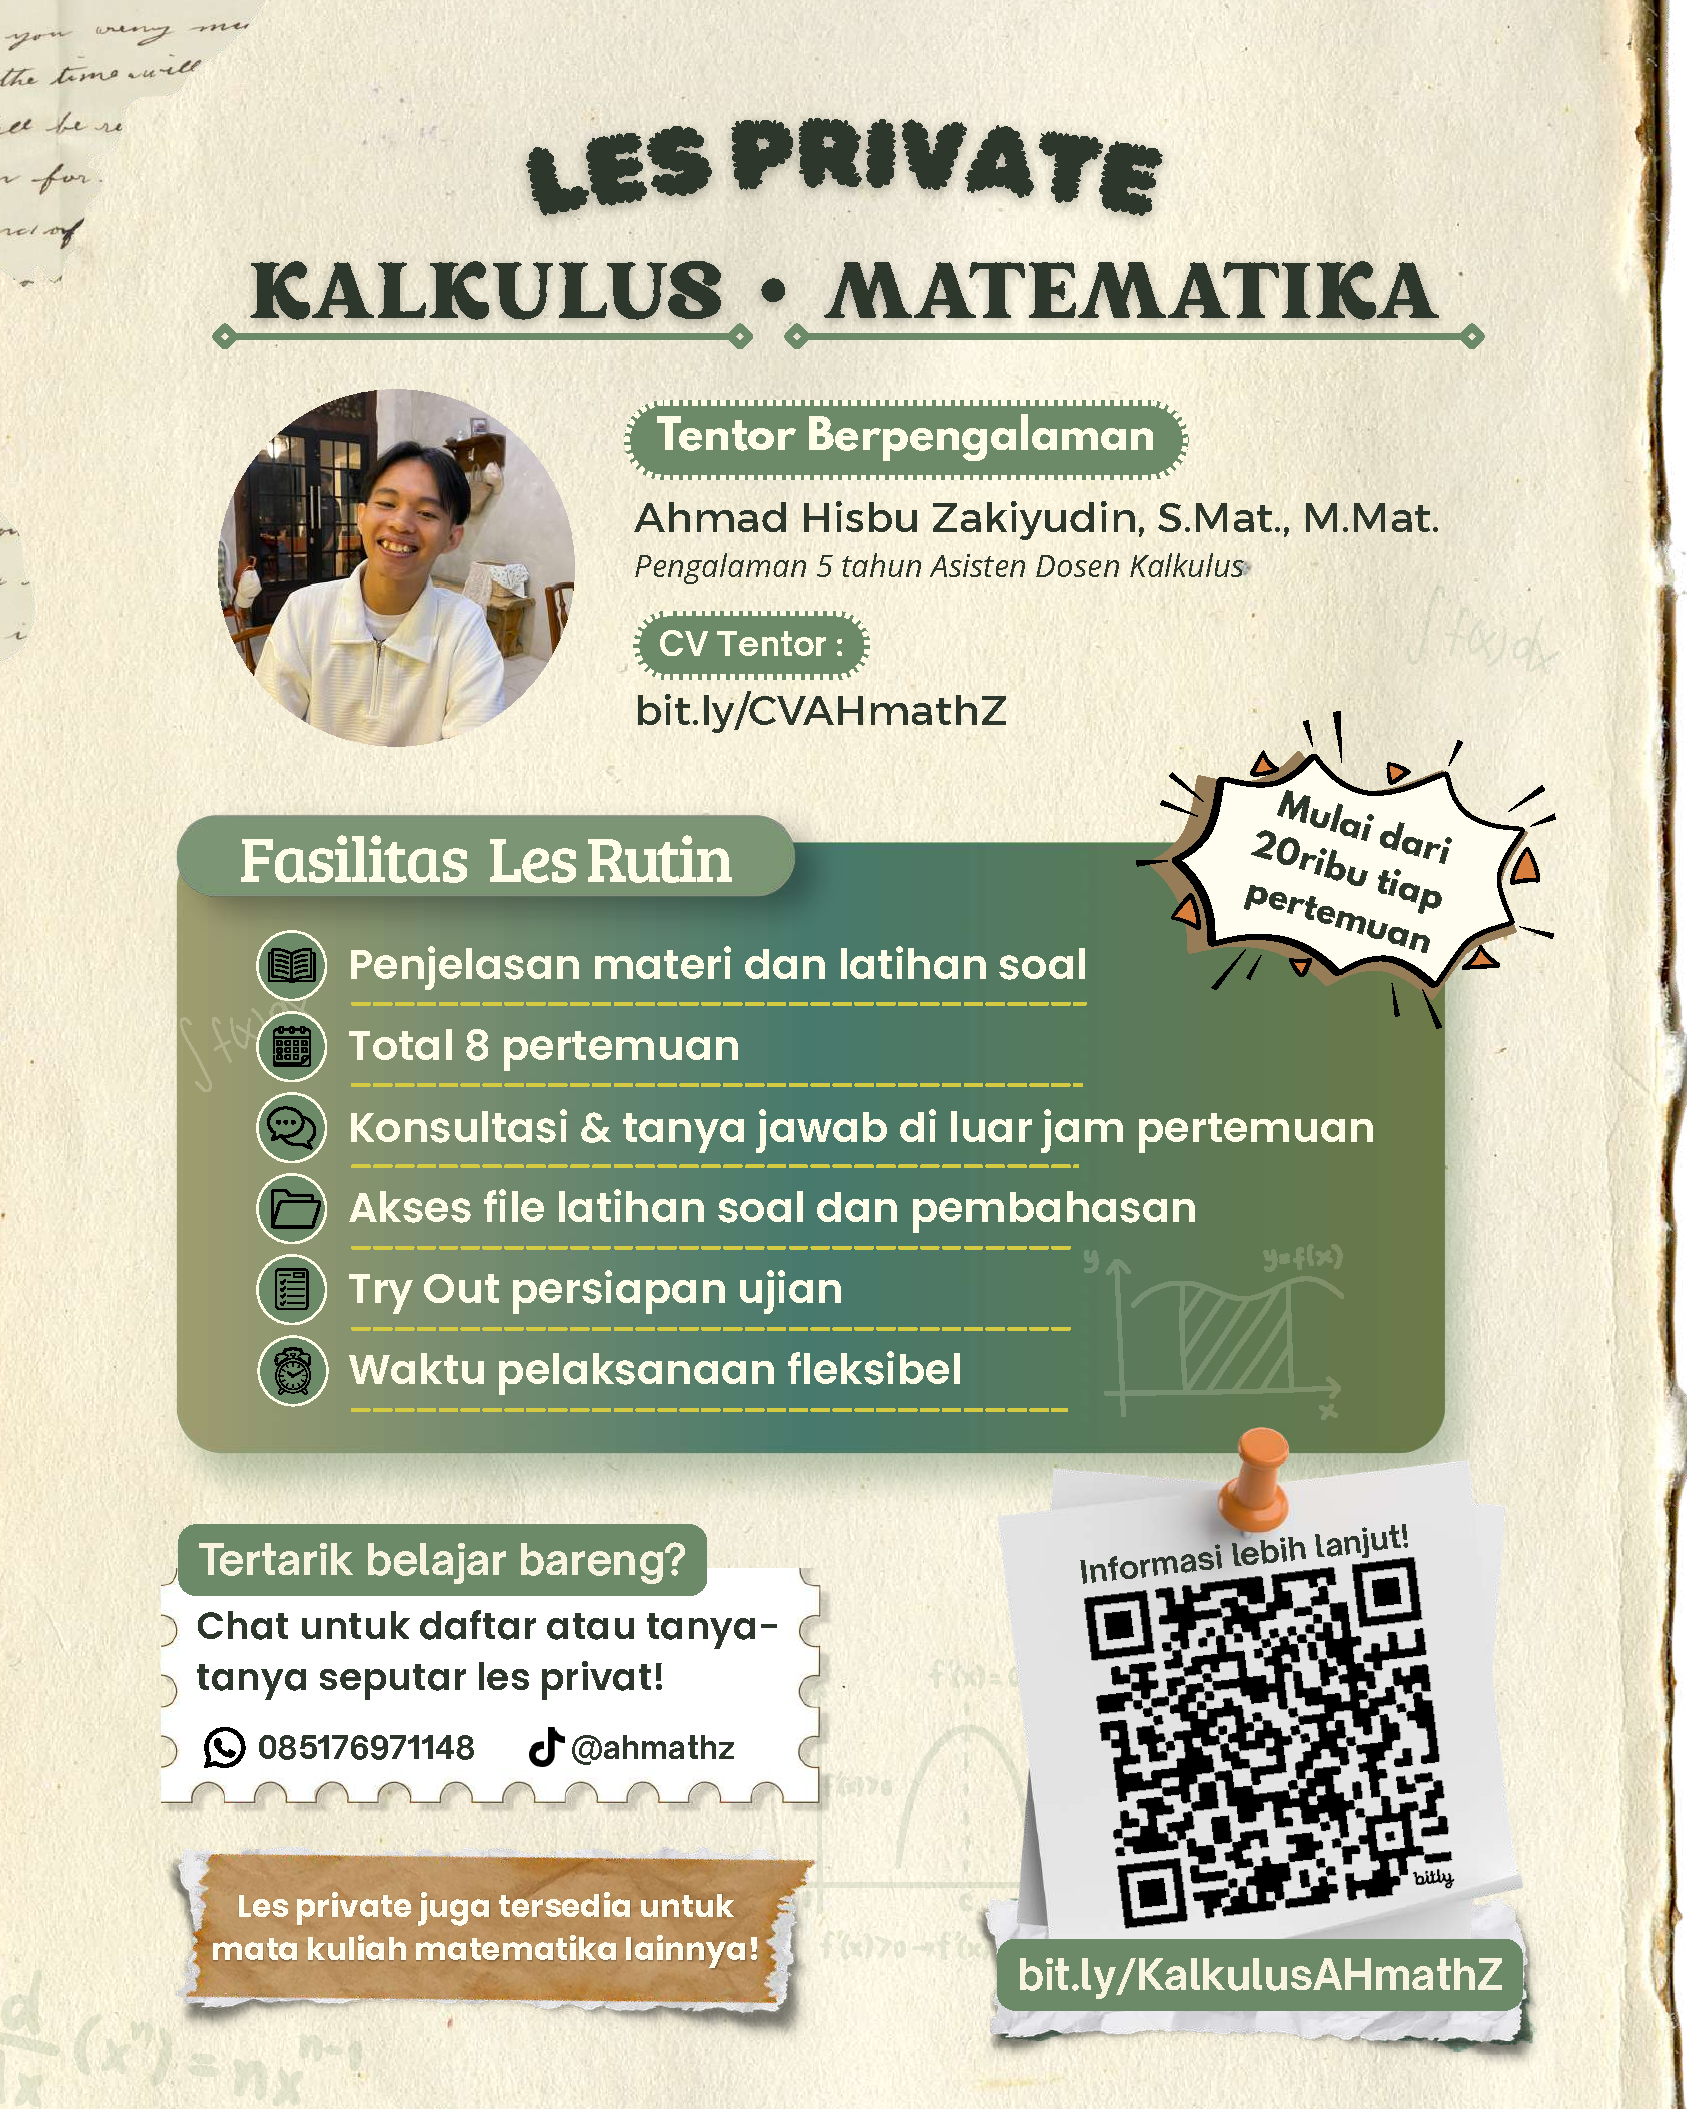
\includepdf{les.pdf}
\setlength\fboxsep{3pt}
% ensure enough header height for fancyhdr
\setlength{\headheight}{24pt}
 \begin{center}
	{\underline{\textbf{\MakeUppercase{Soal dan Pembahasan ETS Kalkulus 1 Tahun 2025/2026}}}}
    \end{center}

    \begin{center}
	\begin{tabular}{lcl}
		Mata kuliah/SKS & : & Kalkulus 1 ( SM234101 ) / 3 SKS\\
		Hari, Tanggal & : & Senin, 13 Oktober 2025\\
		Waktu & : & 07.00 - 08.40 / 100 menit\\
		Sifat & : & Tertutup\\
		Kelas & : & 40-49, 62-66\\
  ~
	\end{tabular}

    \noindent\rule{\textwidth}{2.pt}
        \end{center}
    \begin{enumerate}
     \item Dapatkan semua nilai \(x\) yang memenuhi pertidaksamaan
    \[
        \dfrac{2x + 1}{3x - 6} < \dfrac{1}{2}.
    \]
\begin{jawab}[pertidaksamaan rasional, pecahan, garis bilangan, notasi interval]{~\\
        Untuk menyelesaikan pertidaksamaan rasional, pastikan ruas kanan sudah bernilai nol. Dengan mengurangkan \(\frac{1}{2}\) dari kedua ruas, didapatkan
        \[
        \frac{2x + 1}{3x - 6} - \frac{1}{2} < 0
        \]
        Selanjutnya, dengan menyamakan penyebut dan menyederhanakan bentuknya, diperoleh
        \begin{align}
            \frac{2(2x+1)-(3x-6)}{2(3x-6)} &< 0\nonumber\\
             \frac{4x + 2 - 3x + 6}{2(3x - 6)} &< 0\nonumber \\
             \frac{x + 8}{2(3x - 6)} &< 0 \label{ineq:soal1}
        \end{align}
        Didapatkan pembuat nol dari faktor-faktornya adalah
        \begin{align*}
            x+8 = 0 \quad &\vee\quad  3x - 6 = 0\\
            \colorlet{oldcolor}{.}
        \color{blue}
        \setlength{\fboxrule}{1pt} \boxed{\color{oldcolor}x=-8}\color{oldcolor}
         \quad &\vee\quad \colorlet{oldcolor}{.}
        \color{blue}
        \setlength{\fboxrule}{1pt} \boxed{\color{oldcolor}x=2}\color{oldcolor}
        \end{align*}
        Selanjutnya, dibuat garis bilangan dan dilakukan uji titik pada ekspresi \eqref{ineq:soal1} sebagai berikut
        \begin{itemize}
            \item Untuk \(x < -8\), misalkan \(x = -10\):
            \[
            \frac{-10 + 8}{2(3(-10) - 6)} = \frac{-2}{2(-30 - 6)} = \frac{-2}{2(-36)} = \frac{-2}{-72} > 0
            \]
            \item Untuk \(-8 < x < 2\), misalkan \(x = 0\):
            \[
            \frac{0 + 8}{2(3(0) - 6)} = \frac{8}{2(-6)} = \frac{8}{-12} < 0
            \]
            \item Untuk \(x > 2\), misalkan \(x = 5\):
            \[
            \frac{5 + 8}{2(3(5) - 6)} = \frac{13}{2(15 - 6)} = \frac{13}{2(9)} > 0
            \]
        \end{itemize}
        \begin{center}
           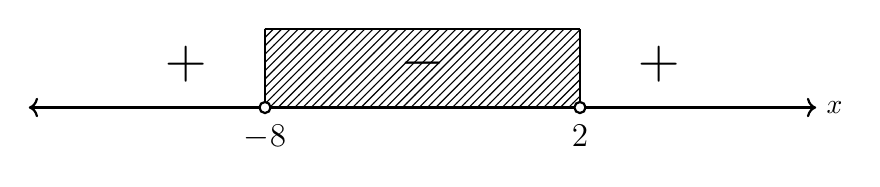
\begin{tikzpicture}
    \draw[thick,<->] (-5,0) -- (5,0) node[right] {$x$};
    \fill[pattern=north east lines] (-2,0) rectangle (2,1);
    \draw (-2,-0.1) node[below] {\large{$-8$}};
    \draw (2,-0.1) node[below] {\large{$2$}};
    \draw[thick] (-2,0) -- (-2,1);
    \draw[thick] (2,0) -- (2,1);
    \draw[thick] (-2,1) -- (2,1);
    \draw (0,0.2) node[above] {\huge{$-$}};
    \draw (3,0.2) node[above] {\huge{$+$}};
    \draw (-3,0.2) node[above] {\huge{$+$}};
    \draw[fill=white, thick] (-2,0) circle (2pt);
    \draw[fill=white, thick] (2,0) circle (2pt);
\end{tikzpicture}
        \end{center}
        Karena yang diminta adalah nilai \(x\) yang membuat pertidaksamaan \eqref{ineq:soal1} kurang dari nol, maka solusi dari pertidaksamaan tersebut adalah \(-8 < x < 2\). Dalam notasi interval, solusi tersebut dapat ditulis sebagai $\colorlet{oldcolor}{.}
        \color{red}
        \setlength{\fboxrule}{1pt} \boxed{\color{oldcolor}(-8, 2)}\color{oldcolor}$.}
    \end{jawab}
    \item Diberikan fungsi \(f(x) = \frac{1}{x-1}\) dan \(g(x) = 2 - \sqrt{x}\).
    \begin{enumerate}
        \item Tentukan domain dari fungsi \(f\) dan \(g\).
        \item Dapatkan fungsi \((f \circ g)(x)\) beserta domainnya.
    \end{enumerate}
    \begin{jawab}[domain fungsi, fungsi komposisi, domain fungsi komposisi]{
        \begin{enumerate}
            \item Diperhatikan bahwa $f(x)$ merupakan fungsi rasional, sehingga domainnya adalah semua bilangan real kecuali nilai yang membuat penyebutnya sama dengan nol, yaitu $x-1\neq 0$. Jadi
            \[
            \colorlet{oldcolor}{.}
        \color{red}
        \setlength{\fboxrule}{1pt} \boxed{\color{oldcolor}D(f)=\{x \in \mathbb{R} : x \neq 1\}}\color{oldcolor}.
            \]
            Selanjutnya, diperhatikan bahwa $g(x)$ memuat akar kuadrat, sehingga domainnya adalah semua bilangan real yang membuat ekspresi di dalam akar kuadrat tak negatif. Jadi
            \[
            \colorlet{oldcolor}{.}
        \color{red}
        \setlength{\fboxrule}{1pt} \boxed{\color{oldcolor}D(g)=\{x \in \mathbb{R} : x \geq 0\}}\color{oldcolor}.
            \]
            \item Diperhatikan bahwa
            \begin{align*}
                (f\circ g)(x) = f(g(x)) = f(2 - \sqrt{x}) = \frac{1}{(2 - \sqrt{x}) - 1} =
                \colorlet{oldcolor}{.}
        \color{red}
        \setlength{\fboxrule}{1pt} \boxed{\color{oldcolor}\frac{1}{1 - \sqrt{x}}}\color{oldcolor}
            \end{align*}
            Domain dari fungsi komposisi $f\circ g$ adalah semua nilai $x$ pada domain $g$ sehingga nilai dari $g(x)$ berada pada domain $f$, yang dapat dirumuskan sebagai
            \begin{align*}
                \colorlet{oldcolor}{.}
        \color{blue}
        \setlength{\fboxrule}{1pt} \boxed{\color{oldcolor}D(f\circ g) = \{x \in D(g) : g(x) \in D(f)\} = \{x \in [0, \infty) : 2 - \sqrt{x} \neq 1\}}\color{oldcolor}.
            \end{align*}
            Karena $2 - \sqrt{x} = 1$ jika dan hanya jika $\sqrt{x} = 1$, yang berarti $x = 1$, didapatkan
            \begin{align*}
                \colorlet{oldcolor}{.}
        \color{red}
        \setlength{\fboxrule}{1pt} \boxed{\color{oldcolor}D(f\circ g) = [0, \infty) \setminus \{1\} = [0, 1) \cup (1, \infty)}\color{oldcolor}.
            \end{align*}
        \end{enumerate}
    }
    \end{jawab}

    \item Diberikan fungsi \(f(x) = \begin{cases} \frac{x^3-8}{2x-4}, & x \neq 2 \\ k, & x=2 \end{cases}\).
    \begin{enumerate}
        \item Tentukan nilai \(k\) sehingga \(f(x)\) kontinu di \(x = 2\).
        \item Berdasarkan hasil dari (a), nyatakan \(f(x)\) sebagai polinomial.
    \end{enumerate}
    \begin{jawab}[fungsi kontinu, limit, polinomial]{
        \begin{enumerate}
            \item Ingat kembali syarat fungsi kontinu di suatu titik \(x = a\) adalah
            \begin{enumerate}
                \item \(f(a)\) terdefinisi
                \item \(\displaystyle \lim_{x \to a} f(x)\) ada, yaitu $\displaystyle \lim_{x \to a^-} f(x) = \lim_{x \to a^+} f(x)$
                \item \(\displaystyle\lim_{x \to a} f(x) = f(a)\)
            \end{enumerate}
            Diperhatikan bahwa untuk \(x = 2\), \(\colorlet{oldcolor}{.}
        \color{blue}
        \setlength{\fboxrule}{1pt} \boxed{\color{oldcolor}f(2) = k~\text{terdefinisi}}\color{oldcolor}\). Karena limit di $x=2$ artinya nilai fungsi di sekitar $x=2$ tetapi $x\neq 2$, didapatkan limitnya adalah
            \begin{align*}
            \lim_{x \to 2} f(x) = \lim_{x \to 2} \frac{x^3 - 8}{2x - 4} = \lim_{x \to 2} \frac{(x-2)(x^2 + 2x + 4)}{2(x-2)} = \lim_{x \to 2} \frac{x^2 + 2x + 4}{2} = \frac{4 + 4 + 4}{2} = \colorlet{oldcolor}{.}
        \color{blue}
        \setlength{\fboxrule}{1pt} \boxed{\color{oldcolor}6}\color{oldcolor}.
            \end{align*}
            Selanjutnya, untuk syarat ketiga, haruslah $\displaystyle \colorlet{oldcolor}{.}
        \color{blue}
        \setlength{\fboxrule}{1pt} \boxed{\color{oldcolor}\lim_{x \to 2} f(x) = f(2)}\color{oldcolor}$, sehingga diperoleh $\colorlet{oldcolor}{.}
        \color{red}
        \setlength{\fboxrule}{1pt} \boxed{\color{oldcolor}k=6}\color{oldcolor}$.
        \item Diperhatikan bahwa untuk $x\neq 2$, berlaku
        \begin{align*}
            f(x) = \frac{x^3 - 8}{2x - 4} = \frac{(x-2)(x^2 + 2x + 4)}{2(x-2)} = \frac{x^2 + 2x + 4}{2} = \frac{1}{2}x^2 + x + 2.
        \end{align*}
        Untuk $x=2$, nilai polinomial tersebut adalah $\frac{1}{2}(4)+2+2=6=k$. Berdasarkan hasil dari (a), diperoleh bahwa \(f(x)\) kontinu di \(x=2\) jika \(k=6\). Dengan demikian, fungsi \(f(x)\) dapat dinyatakan sebagai polinomial
        \begin{align*}
            \colorlet{oldcolor}{.}
        \color{red}
        \setlength{\fboxrule}{1pt} \boxed{\color{oldcolor}f(x) = \frac{1}{2}x^2 + x + 2}\color{oldcolor}.
        \end{align*}
        \end{enumerate}
    }
    \end{jawab}

    \item Diberikan fungsi implisit \(3x^2 + y^2 - 2xy + y - x = 6\). Tentukan \(\frac{dy}{dx}\) di titik \((0,-3)\).
    \begin{jawab}[diferensiasi implisit, turunan, aturan perkalian, aturan rantai]{~\\
        Diperoleh turunan implisit dari fungsi tersebut dengan menurunkan kedua ruas terhadap \(x\):
        \begin{align*}
            \frac{d}{dx}(3x^2 + y^2 - 2xy + y - x) &= \frac{d}{dx}(6)\\
            \frac{d}{dx}(3x^2) + \frac{d}{dx}(y^2) - \frac{d}{dx}(2xy) + \frac{d}{dx}(y) - \frac{d}{dx}(x) &= 0
        \end{align*}
        Untuk suku-suku yang tidak mengandung \(y\), turunan terhadap \(x\) dapat dihitung langsung. Untuk suku-suku yang mengandung \(y\), digunakan aturan rantai dan aturan perkalian. Misalkan $\colorlet{oldcolor}{.}
        \color{blue}
        \setlength{\fboxrule}{1pt} \boxed{\color{oldcolor}p=y^2}\color{oldcolor}$, maka dengan aturan rantai diperoleh
        \begin{align*}
            \colorlet{oldcolor}{.}
        \color{blue}
        \setlength{\fboxrule}{1pt} \boxed{\color{oldcolor}\frac{dp}{dx} = \frac{dp}{dy}\frac{dy}{dx} = 2y\frac{dy}{dx}}\color{oldcolor}
        \end{align*}
        Misalkan $\colorlet{oldcolor}{.}
        \color{blue}
        \setlength{\fboxrule}{1pt} \boxed{\color{oldcolor}u=2x}\color{oldcolor}$ dan $\colorlet{oldcolor}{.}
        \color{blue}
        \setlength{\fboxrule}{1pt}\boxed{\color{oldcolor}v=y}\color{oldcolor}$, maka dengan aturan perkalian diperoleh
        \begin{align*}
        \frac{d}{dx}(2xy)=u'v+uv'=2y + 2x\frac{dy}{dx}= \colorlet{oldcolor}{.}
        \color{blue}
        \setlength{\fboxrule}{1pt} \boxed{\color{oldcolor}2\left(y + x\frac{dy}{dx}\right)}\color{oldcolor}.
        \end{align*}
        Dengan demikian, diperoleh
        \begin{align*}
            6x + 2y\frac{dy}{dx} - 2\left(y + x\frac{dy}{dx}\right) + \frac{dy}{dx} - 1 &= 0\\
            2y\frac{dy}{dx}  - 2x\frac{dy}{dx} + \frac{dy}{dx}  &= 1+2y-6x\\
            (2y - 2x + 1)\frac{dy}{dx} &= 1+2y-6x\\
            \frac{dy}{dx} &=
            \colorlet{oldcolor}{.}
        \color{red}
        \setlength{\fboxrule}{1pt} \boxed{\color{oldcolor}\frac{1+2y-6x}{2y - 2x + 1}}\color{oldcolor}
        \end{align*}
        Selanjutnya, substitusi titik \((0,-3)\) ke dalam persamaan turunan:
        \begin{align*}
            \frac{dy}{dx}\bigg|_{(0,-3)} &= \frac{1+2(-3)-6(0)}{2(-3) - 2(0) + 1}= \frac{1-6}{-6 + 1}= \frac{-5}{-5}= \colorlet{oldcolor}{.}
        \color{red}
        \setlength{\fboxrule}{1pt} \boxed{\color{oldcolor}1}\color{oldcolor}.
        \end{align*}
    }
    \end{jawab}

    \item Diketahui garis \(g_1: y = -x + 6\) dan garis \(g_2: y = 2x\).
    \begin{enumerate}
        \item Tentukan titik potong kedua garis \(g_1\) dan \(g_2\).
        \item Tentukan titik potong \(g_1\) dengan garis \(x = 1\).
        \item Tentukan pula titik potong \(g_2\) dengan garis \(x = 1\). Gambarkan sketsa ketiga garis \(g_1\), \(g_2\), dan garis \(x = 1\). Hitung luas segitiga yang dibentuk ketiga garis tersebut.
    \end{enumerate}
    \begin{jawab}[persamaan garis, titik potong garis, luas segitiga]{
        \begin{enumerate}
            \item Untuk menentukan titik potong kedua garis, kita samakan persamaan kedua garis, yaitu $-x+6=2x$, sehingga $6=3x$, dan diperoleh $x=2$. Selanjutnya, substitusi \(x = 2\) ke dalam salah satu persamaan garis, misalkan \(g_2\), diperoleh $y=2(2)=4$. Jadi titik potong kedua garis adalah \(\colorlet{oldcolor}{.}
        \color{red}
        \setlength{\fboxrule}{1pt} \boxed{\color{oldcolor}(2,4)}\color{oldcolor}\), misalkan sebagai titik $A$.
            \item Untuk menentukan titik potong \(g_1\) dengan garis \(x = 1\), substitusi \(x = 1\) ke dalam persamaan \(g_1\), yaitu $y = -1 + 6 = 5$. Jadi titik potong \(g_1\) dengan garis \(x = 1\) adalah \(\colorlet{oldcolor}{.}
        \color{red}
        \setlength{\fboxrule}{1pt} \boxed{\color{oldcolor}(1,5)}\color{oldcolor}\). Misalkan titik potong tersebut sebagai titik $B$.
            \item Untuk menentukan titik potong \(g_2\) dengan garis \(x = 1\), substitusi \(x = 1\) ke dalam persamaan \(g_2\), yaitu $y = 2(1) = 2$. Jadi titik potong \(g_2\) dengan garis \(x = 1\) adalah \(\colorlet{oldcolor}{.}
        \color{red}
        \setlength{\fboxrule}{1pt} \boxed{\color{oldcolor}(1,2)}\color{oldcolor}\). Misalkan titik potong tersebut sebagai titik $C$.\\
            Dengan melakukan plot titik-titik potong tersebut dan menarik garis di antara dua titik potong, didapatkan sketsa dari ketiga garis dan segitiga tersebut adalah sebagai berikut
            \begin{center}
                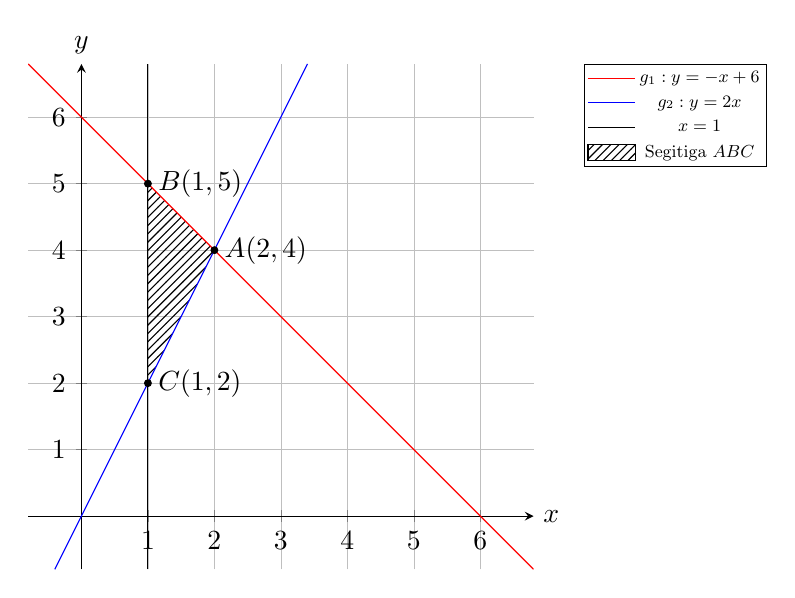
\begin{tikzpicture}
                   \begin{axis}[
        axis lines = middle,
        xlabel = $x$,
        ylabel = {$y$},
        xtick={0,1,...,6},
        ytick={0,1,...,6},
        xmin=-0.8, xmax=6.8,
        ymin=-0.8, ymax=6.8,
        width=8cm,
        height=8cm,
        grid=both,
        grid style={line width=.1pt, draw=gray!10},
        major grid style={line width=.2pt,draw=gray!50},
        x label style={anchor=west}, % label x ke kanan
        y label style={anchor=south}, % label y ke atas
        samples=200,
        legend style={
                at={(1.1,1)},
                anchor=north west,
                font=\small,         % mengecilkan ukuran font
                row sep=1pt,         % jarak antar baris legend
                inner sep=1pt,       % margin dalam kotak legend
                nodes={scale=0.7}    % skalakan isi legend
            }
    ]
\addplot[opacity=0, domain=1:2, name path=A, forget plot] {2*x};
\addplot[opacity=0, domain=1:2, name path=B, forget plot] {-x+6};
\addplot[domain=-0.8:6.8, color=red] {-x+6};
\addlegendentry{$g_1: y=-x+6$}
\addplot[domain=-0.4:3.4, color=blue] {2*x};
\addlegendentry{$g_2: y=2x$}
\addplot[color=black] coordinates {(1,-0.8) (1,6.8)};
\addlegendentry{$x=1$}
\addplot[pattern=north east lines, area legend] fill between[of=A and B, soft clip={domain=1:2}];
\addlegendentry{Segitiga $ABC$}
\draw[fill=black, thick] (2,4) circle (1pt) node[right] {$A(2,4)$};
\draw[fill=black, thick] (1,5) circle (1pt) node[right] {$B(1,5)$};
\draw[fill=black, thick] (1,2) circle (1pt) node[right] {$C(1,2)$};
\end{axis}
                \end{tikzpicture}
            \end{center}
            Pandang garis $BC$ sebagai alas segitiga, sehingga panjang alasnya adalah $|5-2|=\colorlet{oldcolor}{.}
        \color{blue}
        \setlength{\fboxrule}{1pt} \boxed{\color{oldcolor}3}\color{oldcolor}$. Selanjutnya, pandang titik $A$ sebagai titik puncak segitiga, sehingga tinggi segitiga adalah jarak dari titik $A$ ke garis $BC$, yaitu jarak dari titik $(2,4)$ ke garis $x=1$, yang panjangnya adalah $|2-1|=\colorlet{oldcolor}{.}
        \color{blue}
        \setlength{\fboxrule}{1pt} \boxed{\color{oldcolor}1}\color{oldcolor}$. Dengan demikian, luas segitiga tersebut adalah
            \[
            L = \frac{1}{2} \times \text{alas} \times \text{tinggi} = \frac{1}{2} \times 3 \times 1 = \colorlet{oldcolor}{.}
        \color{red}
        \setlength{\fboxrule}{1pt} \boxed{\color{oldcolor}\frac{3}{2}}\color{oldcolor}.
            \]
        \end{enumerate}
    }
    \end{jawab}
\end{enumerate}
\newpage
 \begin{center}
	{\underline{\textbf{\MakeUppercase{Soal dan Pembahasan ETS Kalkulus 1 Tahun 2025/2026}}}}
    \end{center}

    \begin{center}
	\begin{tabular}{lcl}
		Course / Credit & : & Kalkulus 1 ( SM234101 ) / 3 SKS\\
		Day, Date & : & Monday, 13 October 2025\\
		Time / Exam Time & : & 09.00 - 10.40 / 100 menit\\
		Type & : & Tertutup\\
		Class & : & 1, 4, 67, 70, 71\\
  ~
	\end{tabular}

    \noindent\rule{\textwidth}{2.pt}
        \end{center}
\begin{enumerate}
           \item Solve the following inequality.
    \[\frac{x^2 - x - 12}{x^2 - 2x - 3} \ge 0. \]
    \begin{jawab}[pertidaksamaan rasional, persamaan kuadrat, notasi interval]{~\\
    Karena ruas kanan pertidaksamaan sudah bernilai nol, maka kita bisa langsung memfaktorkan pembilang dan penyebut di ruas kiri. Diperoleh
    \begin{align*}
        \frac{x^2 - x - 12}{x^2 - 2x - 3} &= \frac{(x-4)(x+3)}{(x-3)(x+1)} \ge 0
    \end{align*}
    Selanjutnya, kita tentukan pembuat nol dari faktor-faktor tersebut, yaitu
    \begin{align*}
        x-4 = 0 \quad &\vee\quad x+3 = 0 \quad \vee\quad x-3 = 0 \quad \vee\quad x+1 = 0\\
        \colorlet{oldcolor}{.}
        \color{blue}
        \setlength{\fboxrule}{1pt} \boxed{\color{oldcolor}x=4}\color{oldcolor} \quad &\vee\quad \colorlet{oldcolor}{.}
        \color{blue}
        \setlength{\fboxrule}{1pt} \boxed{\color{oldcolor}x=-3}\color{oldcolor} \quad \vee\quad \colorlet{oldcolor}{.}
        \color{blue}
        \setlength{\fboxrule}{1pt} \boxed{\color{oldcolor}x=3}\color{oldcolor} \quad \vee\quad \colorlet{oldcolor}{.}
        \color{blue}
        \setlength{\fboxrule}{1pt} \boxed{\color{oldcolor}x=-1}\color{oldcolor}
    \end{align*}
    Selanjutnya, kita buat garis bilangan dan lakukan uji titik pada ekspresi \(\frac{(x-4)(x+3)}{(x-3)(x+1)}\) sebagai berikut
    \begin{itemize}
        \item Untuk \(x < -3\), misalkan \(x = -4\):
        \[
        \frac{(-4-4)(-4+3)}{(-4-3)(-4+1)} = \frac{(-8)(-1)}{(-7)(-3)} = \frac{8}{21} > 0
        \]
        \item Untuk \(-3 < x < -1\), misalkan \(x = -2\):
        \[
        \frac{(-2-4)(-2+3)}{(-2-3)(-2+1)} = \frac{(-6)(1)}{(-5)(-1)} = \frac{-6}{5} < 0
        \]
        \item Untuk \(-1 < x < 3\), misalkan \(x = 0\):
        \[
        \frac{(0-4)(0+3)}{(0-3)(0+1)} = \frac{(-4)(3)}{(-3)(1)} = \frac{-12}{-3} = 4 > 0
        \]
        \item Untuk \(3 < x < 4\), misalkan \(x = 3.5\):
        \[
        \frac{(3.5-4)(3.5+3)}{(3.5-3)(3.5+1)} = \frac{(-0.5)(6.5)}{(0.5)(4.5)} = \frac{-3.25}{2.25} < 0
        \]
        \item Untuk \(x > 4\), misalkan \(x = 5\):
        \[
        \frac{(5-4)(5+3)}{(5-3)(5+1)} = \frac{(1)(8)}{(2)(6)} = \frac{8}{12} = \frac{2}{3} > 0
        \]
    \end{itemize}
    \begin{center}
        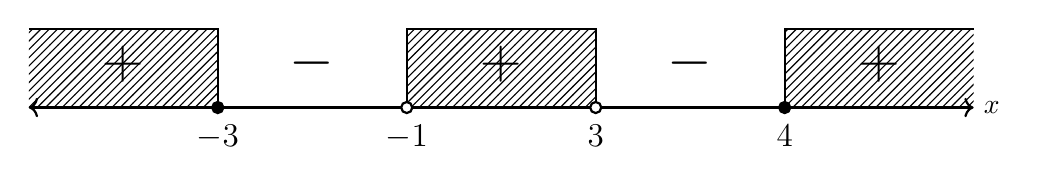
\begin{tikzpicture}
    \draw[thick,<->] (-6,0) -- (6,0) node[right] {$x$};
    \fill[pattern=north east lines] (-6,0) rectangle (-3.6,1);
    \fill[pattern=north east lines] (-1.2,0) rectangle (1.2,1);
    \fill[pattern=north east lines] (3.6,0) rectangle (6,1);
    \draw[thick] (-6,1) -- (-3.6,1) -- (-3.6,0);
    \draw[thick] (-1.2,0) -- (-1.2,1) -- (1.2,1) -- (1.2,0);
    \draw[thick] (3.6,0) -- (3.6,1) -- (6,1);
    \draw (-3.6,-0.1) node[below] {\large{$-3$}};
    \draw (-1.2,-0.1) node[below] {\large{$-1$}};
    \draw (1.2,-0.1) node[below] {\large{$3$}};
    \draw (3.6,-0.1) node[below] {\large{$4$}};
    \draw (-4.8,0.2) node[above] {\huge{$+$}};
    \draw (-2.4,0.2) node[above] {\huge{$-$}};
    \draw (0,0.2) node[above] {\huge{$+$}};
    \draw (2.4,0.2) node[above] {\huge{$-$}};
    \draw (4.8,0.2) node[above] {\huge{$+$}};
    \draw[fill=black, thick] (-3.6,0) circle (2pt);
    \draw[fill=white, thick] (-1.2,0) circle (2pt);
    \draw[fill=white, thick] (1.2,0) circle (2pt);
    \draw[fill=black, thick] (3.6,0) circle (2pt);
        \end{tikzpicture}
    \end{center}
    Karena yang diminta adalah nilai yang lebih dari atau sama dengan nol, diambil interval yang bertanda positif beserta pembuat nol dari pembilang ($x=-3$ dan $x=4$). Pembuat nol dari penyebut ($x=-1$ dan $x=3$) tidak diikutkan karena membuat ekspresi tidak terdefinisi. Jadi solusi dari pertidaksamaan tersebut adalah \(x \leq -3\) atau \(-1 < x < 3\) atau \(x \geq 4\). Dalam notasi interval, solusi tersebut dapat ditulis sebagai $\colorlet{oldcolor}{.}
        \color{red}
        \setlength{\fboxrule}{1pt} \boxed{\color{oldcolor}(-\infty, -3] \cup (-1, 3) \cup [4, \infty)}\color{oldcolor}$.
    }
    \end{jawab}

    \item Given a function \(f(x) = 2 - \sqrt{x}\) and \(g(x) = \frac{1}{x-1}\). Determine:
    \begin{enumerate}
        \item[a)] The domain of function \(f\) and \(g\);
        \item[b)] Function \((f \circ g)(x)\) and its domain.
    \end{enumerate}
    \begin{jawab}[domain fungsi, fungsi komposisi, domain fungsi komposisi]{
        \begin{enumerate}
            \item Diperhatikan bahwa $f(x)$ memuat akar kuadrat, sehingga domainnya adalah semua bilangan real yang membuat ekspresi di dalam akar kuadrat tak negatif. Jadi
            \begin{align*}
                \colorlet{oldcolor}{.}
        \color{red}
        \setlength{\fboxrule}{1pt} \boxed{\color{oldcolor}D(f)=\{x \in \mathbb{R} : x \geq 0\}}\color{oldcolor}.
            \end{align*}
            Selanjutnya, diperhatikan bahwa $g(x)$ merupakan fungsi rasional, sehingga domainnya adalah semua bilangan real kecuali nilai yang membuat penyebutnya sama dengan nol, yaitu $x-1\neq 0$. Jadi
            \begin{align*}
                \colorlet{oldcolor}{.}
        \color{red}
        \setlength{\fboxrule}{1pt} \boxed{\color{oldcolor}D(g)=\{x \in \mathbb{R} : x \neq 1\}}\color{oldcolor}.
            \end{align*}
            \item Diperhatikan bahwa
            \begin{align*}
                (f\circ g)(x) = f(g(x)) = f\left(\frac{1}{x-1}\right) = 2 - \sqrt{\frac{1}{x-1}} = \colorlet{oldcolor}{.}
        \color{red}
        \setlength{\fboxrule}{1pt} \boxed{\color{oldcolor}2 - \frac{1}{\sqrt{x-1}}}\color{oldcolor}
            \end{align*}
            Domain dari fungsi komposisi $f\circ g$ adalah semua nilai $x$ pada domain $g$ sehingga nilai dari $g(x)$ berada pada domain $f$, yang dapat dirumuskan sebagai
            \begin{align*}
                \colorlet{oldcolor}{.}
        \color{blue}
        \setlength{\fboxrule}{1pt} \boxed{\color{oldcolor}D(f\circ g) = \{x \in D(g) : g(x) \in D(f)\} = \left\{x \neq 1 : \frac{1}{x-1} \geq 0\right\}}\color{oldcolor}.
            \end{align*}
            Karena pembilangnya bernilai $1>0$, maka $\frac{1}{x-1} \geq 0$ jika dan hanya jika $x-1 > 0$, yang berarti $x > 1$. Didapatkan
            \begin{align*}
                \colorlet{oldcolor}{.}
        \color{red}
        \setlength{\fboxrule}{1pt} \boxed{\color{oldcolor}D(f\circ g) = (1, \infty)}\color{oldcolor}.
            \end{align*}
        \end{enumerate}
    }
    \end{jawab}

    \item Write the derivative formula of \(\frac{f}{g}\), that is \(\frac{d}{dx}\left(\frac{f(x)}{g(x)}\right)\). \\
    Then, find the derivative of \(\frac{f}{g}\) given that \(f(x) = 2x^2 + 3x - 2\) and \(g(x) = x - 1\) for \(x \neq 1\).
    \begin{jawab}[turunan, aturan pembagian]{~\\
        Ingat kembali aturan turunan untuk pembagian fungsi, yaitu
        \[
        \colorlet{oldcolor}{.}
        \color{red}
        \setlength{\fboxrule}{1pt} \boxed{\color{oldcolor}\frac{d}{dx}\left(\frac{f(x)}{g(x)}\right) = \frac{f'(x)g(x) - f(x)g'(x)}{(g(x))^2}}\color{oldcolor}.
        \]
        Selanjutnya, kita hitung turunan dari \(f(x)\) dan \(g(x)\):
        \begin{align*}
            \colorlet{oldcolor}{.}
        \color{blue}
        \setlength{\fboxrule}{1pt} \boxed{\color{oldcolor}f'(x) = \frac{d}{dx}(2x^2 + 3x - 2) = 4x + 3}\color{oldcolor}\\
            \colorlet{oldcolor}{.}
        \color{blue}
        \setlength{\fboxrule}{1pt} \boxed{\color{oldcolor}g'(x) = \frac{d}{dx}(x - 1) = 1}\color{oldcolor}
        \end{align*}
        Dengan demikian, turunan dari \(\frac{f}{g}\) adalah
        \begin{align*}
            \frac{d}{dx}\left(\frac{f(x)}{g(x)}\right) &= \frac{(4x + 3)(x - 1) - (2x^2 + 3x - 2)(1)}{(x - 1)^2}\\
            &= \frac{(4x^2 - 4x + 3x - 3) - (2x^2 + 3x - 2)}{(x - 1)^2}\\
            &= \frac{4x^2 - x - 3 - 2x^2 - 3x + 2}{(x - 1)^2}\\
            &= \colorlet{oldcolor}{.}
        \color{red}
        \setlength{\fboxrule}{1pt} \boxed{\color{oldcolor}\frac{2x^2 - 4x - 1}{(x - 1)^2}}\color{oldcolor}.
        \end{align*}
    }
    \end{jawab}

    \item Given \(f(x) = \begin{cases} \frac{x^3-8}{2x-4}, & x \neq 2 \\ 2k, & x=2 \end{cases}\).
    \begin{enumerate}
        \item[a.] Determine k such that \(f(x)\) continuous at \(x = 2\).
        \item[b.] Based on the result of a), rewrite \(f(x)\) as a polynomial.
    \end{enumerate}
    \begin{jawab}[fungsi kontinu, limit, polinomial]{
        \begin{enumerate}
            \item Ingat kembali syarat fungsi kontinu di suatu titik \(x = a\) adalah
            \begin{enumerate}
                \item \(f(a)\) terdefinisi
                \item \(\displaystyle \lim_{x \to a} f(x)\) ada, yaitu $\displaystyle \lim_{x \to a^-} f(x) = \lim_{x \to a^+} f(x)$
                \item \(\displaystyle\lim_{x \to a} f(x) = f(a)\)
            \end{enumerate}
            Diperhatikan bahwa untuk \(x = 2\), $\colorlet{oldcolor}{.}
        \color{blue}
        \setlength{\fboxrule}{1pt} \boxed{\color{oldcolor}f(2) = 2k~\text{terdefinisi}}\color{oldcolor}$. Karena limit di $x=2$ artinya nilai fungsi di sekitar $x=2$ tetapi $x\neq 2$, didapatkan limitnya adalah
            \begin{align*}
            \lim_{x \to 2} f(x) = \lim_{x \to 2} \frac{x^3 - 8}{2x - 4} = \lim_{x \to 2} \frac{(x-2)(x^2 + 2x + 4)}{2(x-2)} = \lim_{x \to 2} \frac{x^2 + 2x + 4}{2} = \colorlet{oldcolor}{.}
        \color{blue}
        \setlength{\fboxrule}{1pt} \boxed{\color{oldcolor}6}\color{oldcolor}.
            \end{align*}
            Selanjutnya, untuk syarat ketiga, haruslah $\displaystyle\lim_{x \to 2} f(x) = f(2)$, sehingga diperoleh $6 = 2k$, dan didapatkan $\colorlet{oldcolor}{.}
        \color{red}
        \setlength{\fboxrule}{1pt} \boxed{\color{oldcolor}k=3}\color{oldcolor}$.
        \item Diperhatikan bahwa untuk $x\neq 2$, berlaku
        \begin{align*}
            f(x) = \frac{x^3 - 8}{2x - 4} = \frac{(x-2)(x^2 + 2x + 4)}{2(x-2)} = \frac{x^2 + 2x + 4}{2} = \frac{1}{2}x^2 + x + 2.
        \end{align*}
        Berdasarkan hasil dari (a), diperoleh bahwa \(f(x)\) kontinu di \(x=2\) jika \(k=3\), yaitu $f(2)=6$, yang sama dengan nilai polinomial di atas saat $x=2$. Dengan demikian, fungsi \(f(x)\) dapat dinyatakan sebagai polinomial
        \begin{align*}
            \colorlet{oldcolor}{.}
        \color{red}
        \setlength{\fboxrule}{1pt} \boxed{\color{oldcolor}f(x) = \frac{1}{2}x^2 + x + 2}\color{oldcolor}.
        \end{align*}
        \end{enumerate}
    }
    \end{jawab}

    \item Sketch the base curve \(x = y^2\). Based on that base curve, use translation to sketch the curve \(x = y^2 + 4y + 1\). (Explain the process).
    \begin{jawab}[parabola, melengkapkan kuadrat, translasi grafik]{~\\
        Kurva dasar $x=y^2$ merupakan parabola yang terbuka ke kanan dengan titik puncak $(0,0)$. Selanjutnya, bentuk $x = y^2 + 4y + 1$ diubah dengan cara melengkapkan kuadrat, yaitu
        \begin{align*}
            x &= y^2 + 4y + 1\\
            &= (y^2 + 4y + 4) - 4 + 1\\
            &= \colorlet{oldcolor}{.}
        \color{blue}
        \setlength{\fboxrule}{1pt} \boxed{\color{oldcolor}(y+2)^2 - 3}\color{oldcolor}.
        \end{align*}
        Ingat kembali bahwa mengganti $y$ dengan $y+2$ berarti menggeser grafik sejauh $2$ satuan ke bawah, dan menambahkan konstanta $-3$ pada $x$ berarti menggeser grafik sejauh $3$ satuan ke kiri. Dengan demikian, proses translasinya adalah sebagai berikut.
        \begin{enumerate}
            \item[(i)] Gambar kurva dasar $x=y^2$ dengan titik puncak $(0,0)$.
            \item[(ii)] Geser kurva $x=y^2$ sejauh $2$ satuan ke bawah, sehingga diperoleh kurva $x=(y+2)^2$ dengan titik puncak $(0,-2)$.
            \item[(iii)] Geser kurva $x=(y+2)^2$ sejauh $3$ satuan ke kiri, sehingga diperoleh kurva $x=(y+2)^2-3$ dengan titik puncak $\colorlet{oldcolor}{.}
        \color{blue}
        \setlength{\fboxrule}{1pt} \boxed{\color{oldcolor}(-3,-2)}\color{oldcolor}$.
        \end{enumerate}
        Sebagai bantuan, titik potong kurva dengan sumbu-$x$ ($y=0$) adalah $x=1$, yaitu titik $(1,0)$, sedangkan titik potong dengan sumbu-$y$ ($x=0$) adalah $(y+2)^2=3$, yaitu $y=-2\pm\sqrt{3}$. Sketsa grafiknya adalah sebagai berikut.
        \begin{center}
            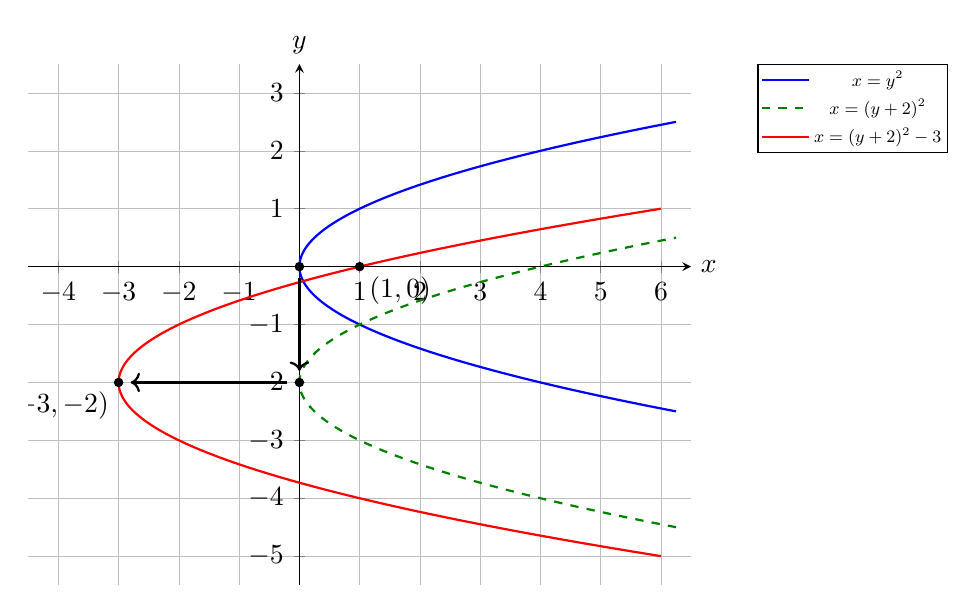
\begin{tikzpicture}
                \begin{axis}[
        axis lines = middle,
        xlabel = $x$,
        ylabel = {$y$},
        xtick={-4,-3,...,6},
        ytick={-5,-4,...,3},
        xmin=-4.5, xmax=6.5,
        ymin=-5.5, ymax=3.5,
        width=10cm,
        height=8.2cm,
        grid=both,
        grid style={line width=.1pt, draw=gray!10},
        major grid style={line width=.2pt,draw=gray!50},
        x label style={anchor=west}, % label x ke kanan
        y label style={anchor=south}, % label y ke atas
        samples=200,
        legend style={
                at={(1.1,1)},
                anchor=north west,
                font=\small,         % mengecilkan ukuran font
                row sep=1pt,         % jarak antar baris legend
                inner sep=1pt,       % margin dalam kotak legend
                nodes={scale=0.7}    % skalakan isi legend
            }
    ]
\addplot[domain=-2.5:2.5, color=blue, thick] ({(x)*(x)},{x});
\addlegendentry{$x=y^2$}
\addplot[domain=-4.5:0.5, color=green!50!black, thick, dashed] ({(x+2)*(x+2)},{x});
\addlegendentry{$x=(y+2)^2$}
\addplot[domain=-5:1, color=red, thick] ({(x+2)*(x+2)-3},{x});
\addlegendentry{$x=(y+2)^2-3$}
\draw[fill=black] (0,0) circle (1.5pt);
\draw[fill=black] (0,-2) circle (1.5pt);
\draw[fill=black] (-3,-2) circle (1.5pt) node[below left] {$(-3,-2)$};
\draw[fill=black] (1,0) circle (1.5pt) node[below right] {$(1,0)$};
\draw[->, thick] (0,-0.2) -- (0,-1.8);
\draw[->, thick] (-0.2,-2) -- (-2.8,-2);
\end{axis}
            \end{tikzpicture}
        \end{center}
        Jadi kurva $x = y^2 + 4y + 1$ adalah
        \[\colorlet{oldcolor}{.}
        \color{red}
        \setlength{\fboxrule}{1pt} \boxed{\color{oldcolor}\text{parabola } x=y^2 \text{ yang digeser 2 satuan ke bawah dan 3 satuan ke kiri}}\color{oldcolor}.\]
    }
    \end{jawab}
        \end{enumerate}
               \newpage
 \begin{center}
	{\underline{\textbf{\MakeUppercase{Soal dan Pembahasan ETS Kalkulus 1 Tahun 2025/2026}}}}
    \end{center}

    \begin{center}
	\begin{tabular}{lcl}
		Mata kuliah/SKS & : & Kalkulus 1 ( SM234101 ) / 3 SKS\\
		Hari, Tanggal & : & Senin, 13 Oktober 2025\\
		Waktu & : & 11.00 - 12.40 / 100 menit\\
		Sifat & : & Tertutup\\
		Kelas & : & 17-22\\
  ~
	\end{tabular}

    \noindent\rule{\textwidth}{2.pt}
        \end{center}
\begin{enumerate}
    \item \begin{enumerate}
        \item Nyatakan pernyataan $\sqrt{(2x-1)^2}$ dalam bentuk nilai mutlak.
        \item Dapatkan semua nilai $x$ yang memenuhi persamaan $\sqrt{(2x-1)^2}=1-2x$.
    \end{enumerate}
    \begin{jawab}[definisi nilai mutlak, persamaan nilai mutlak]{
        \begin{enumerate}
            \item Ingat bahwa $\sqrt{x^2}=|x|$, sehingga diperoleh
            \begin{align*}
                \colorlet{oldcolor}{.}
        \color{red}
        \setlength{\fboxrule}{1pt} \boxed{\color{oldcolor}\sqrt{(2x-1)^2} = |2x-1|}\color{oldcolor}.
            \end{align*}
            \item Diperhatikan bahwa
            \begin{align*}
                |2x-1| = 1-2x = -(2x-1)
            \end{align*}
            Kemudian, pertimbangkan definisi nilai mutlak, yaitu
            \begin{align*}
                |2x-1| = \begin{cases}
                    2x-1, & 2x-1 \geq 0\\
                    -(2x-1), & 2x-1 < 0
                \end{cases}
            \end{align*}
            Berdasarkan definisi tersebut, didapatkan bahwa persamaan $|2x-1| = -(2x-1)$ berlaku jika $2x-1 < 0$, yang berarti $x < \frac{1}{2}$. Selain itu, pada batasnya, yaitu $x=\frac{1}{2}$, diperoleh $|0| = 0 = -0$, sehingga $x=\frac{1}{2}$ juga memenuhi persamaan. Jadi semua nilai $x$ yang memenuhi persamaan tersebut adalah $\colorlet{oldcolor}{.}
        \color{red}
        \setlength{\fboxrule}{1pt} \boxed{\color{oldcolor}x \leq \frac{1}{2}}\color{oldcolor}$.
        \end{enumerate}
    }
    \end{jawab}
    \item Diberikan fungsi $f(x)=\sqrt{x-4}$.
    \begin{enumerate}
        \item Tentukan domain dan range dari fungsi $f(x)$.
        \item Tentukan $f^{-1}(x)$, domain dan range dari $f^{-1}(x)$.
    \end{enumerate}
    \begin{jawab}[domain dan range fungsi, fungsi invers]{
        \begin{enumerate}
            \item Diperhatikan bahwa $f(x)$ memuat akar kuadrat, sehingga domainnya adalah semua bilangan real yang membuat ekspresi di dalam akar kuadrat tak negatif. Jadi
            \begin{align*}
                \colorlet{oldcolor}{.}
        \color{red}
        \setlength{\fboxrule}{1pt} \boxed{\color{oldcolor}D(f)=\{x \in \mathbb{R} : x-4 \geq 0\} = [4, \infty)}\color{oldcolor}.
            \end{align*}
            Selanjutnya, karena $f(x)$ merupakan fungsi akar kuadrat, maka nilainya selalu tak negatif, dan untuk $x$ yang membesar dari $4$, nilai $\sqrt{x-4}$ membesar dari $0$ tanpa batas. Jadi
            \begin{align*}
                \colorlet{oldcolor}{.}
        \color{red}
        \setlength{\fboxrule}{1pt} \boxed{\color{oldcolor}R(f)=\{y \in \mathbb{R} : y \geq 0\} = [0, \infty)}\color{oldcolor}.
            \end{align*}
            \item Untuk mendapatkan fungsi invers dari $f(x)$, kita misalkan $y=f(x)$, kemudian selesaikan sehingga terbentuk $x$ dalam fungsi $y$. Diperoleh
            \begin{align*}
                y &= f(x) = \sqrt{x-4}\\
                y^2 &= x-4\\
                x &= y^2 + 4.
            \end{align*}
            Dari sini didapatkan $x = f^{-1}(y) = y^2 + 4$. Dengan mengganti $y$ dengan $x$, diperoleh
            \begin{align*}
                f^{-1}(x) = x^2 + 4.
            \end{align*}
            Selanjutnya, domain dari fungsi invers adalah range dari fungsi asli, yaitu $\colorlet{oldcolor}{.}
        \color{blue}
        \setlength{\fboxrule}{1pt} \boxed{\color{oldcolor}D(f^{-1}) = R(f) = [0, \infty)}\color{oldcolor}$, serta range dari fungsi invers adalah domain dari fungsi asli, yaitu $\colorlet{oldcolor}{.}
        \color{blue}
        \setlength{\fboxrule}{1pt} \boxed{\color{oldcolor}R(f^{-1}) = D(f) = [4, \infty)}\color{oldcolor}$. Jadi fungsi inversnya adalah
        \begin{align*}
            \colorlet{oldcolor}{.}
        \color{red}
        \setlength{\fboxrule}{1pt} \boxed{\color{oldcolor}f^{-1}(x) = x^2 + 4,\quad x\geq 0}\color{oldcolor}.
        \end{align*}
        \end{enumerate}
    }
    \end{jawab}
    \item Diberikan persamaan separuh lingkaran
    \begin{align*}
       x=4+\sqrt{-y^2+14y-24}.
    \end{align*}
    \begin{enumerate}
        \item Dapatkan pusat dan jari-jari lingkaran.
        \item Sketsa grafiknya.
    \end{enumerate}
    \begin{jawab}[persamaan lingkaran, pusat dan jari-jari lingkaran, sketsa grafik]{
        \begin{enumerate}
            \item Diperhatikan bahwa persamaan tersebut dapat ditulis ulang menjadi
            \begin{align*}
                x-4 &= \sqrt{-y^2+14y-24}\\
                (x-4)^2 &= -y^2+14y-24\\
                (x-4)^2 + y^2 - 14y + 24 &= 0\\
                (x-4)^2 + (y^2 - 14y + 49) - 49 + 24 &= 0\\
                (x-4)^2 + (y-7)^2 - 25 &= 0\\
                (x-4)^2 + (y-7)^2 &= 25.
            \end{align*}
            Dari persamaan tersebut, dapat dilihat bahwa pusat lingkaran adalah $(4,7)$ dan jari-jari lingkaran adalah $\sqrt{25} = 5$. Jadi pusat dan jari-jari lingkaran adalah $\colorlet{oldcolor}{.}
        \color{red}
        \setlength{\fboxrule}{1pt} \boxed{\color{oldcolor}\text{Pusat: }(4,7),~\text{Jari-jari: }5}\color{oldcolor}$.
            \item Sketsa grafik untuk lingkaran penuhnya adalah sebagai berikut:
            \begin{center}
                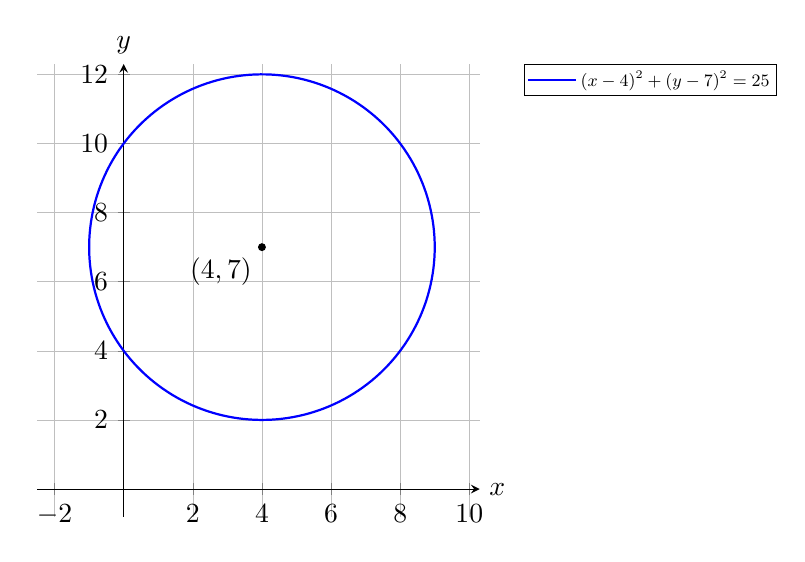
\begin{tikzpicture}
                   \begin{axis}[
        axis lines = middle,
        xlabel = $x$,
        ylabel = {$y$},
        xtick={-2,0,...,10},
        ytick={0,2,...,12},
        xmin=-2.5, xmax=10.3,
        ymin=-0.8, ymax=12.3,
        axis equal image,
        width=8.5cm,
        grid=both,
        grid style={line width=.1pt, draw=gray!10},
        major grid style={line width=.2pt,draw=gray!50},
        x label style={anchor=west}, % label x ke kanan
        y label style={anchor=south}, % label y ke atas
        samples=200,
        legend style={
                at={(1.1,1)},
                anchor=north west,
                font=\small,         % mengecilkan ukuran font
                row sep=1pt,         % jarak antar baris legend
                inner sep=1pt,       % margin dalam kotak legend
                nodes={scale=0.7}    % skalakan isi legend
            }
    ]
\addplot[domain=0:360, color=blue, thick] ({4+5*cos(x)}, {7+5*sin(x)});
\addlegendentry{$(x-4)^2+(y-7)^2=25$}
\draw[fill=black, thick] (4,7) circle (1pt) node[anchor=north east] {$(4,7)$};
\end{axis}
                \end{tikzpicture}
            \end{center}
            Diperhatikan bahwa pada persamaan $x=4+\sqrt{-y^2+14y-24}$ berlaku $x-4=\sqrt{-y^2+14y-24}\geq 0$, artinya $x\geq 4$. Sehingga sketsa grafik separuh lingkaran yang diberikan dalam soal merupakan bagian kanan dari lingkaran, yaitu sebagai berikut:
            \begin{center}
                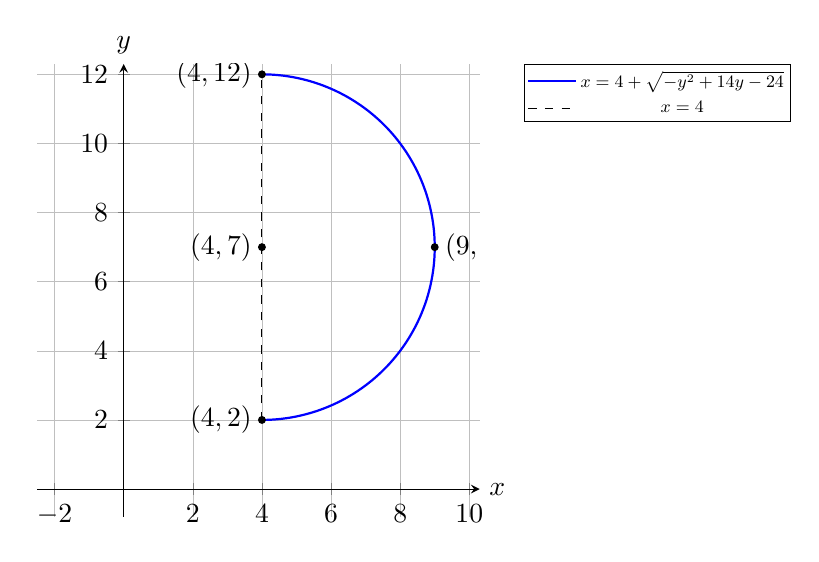
\begin{tikzpicture}
                   \begin{axis}[
        axis lines = middle,
        xlabel = $x$,
        ylabel = {$y$},
        xtick={-2,0,...,10},
        ytick={0,2,...,12},
        xmin=-2.5, xmax=10.3,
        ymin=-0.8, ymax=12.3,
        axis equal image,
        width=8.5cm,
        grid=both,
        grid style={line width=.1pt, draw=gray!10},
        major grid style={line width=.2pt,draw=gray!50},
        x label style={anchor=west}, % label x ke kanan
        y label style={anchor=south}, % label y ke atas
        samples=200,
        legend style={
                at={(1.1,1)},
                anchor=north west,
                font=\small,         % mengecilkan ukuran font
                row sep=1pt,         % jarak antar baris legend
                inner sep=1pt,       % margin dalam kotak legend
                nodes={scale=0.7}    % skalakan isi legend
            }
    ]
\addplot[domain=-90:90, color=blue, thick] ({4+5*cos(x)}, {7+5*sin(x)});
\addlegendentry{$x=4+\sqrt{-y^2+14y-24}$}
\addplot[color=black, dashed] coordinates {(4,2) (4,12)};
\addlegendentry{$x=4$}
\draw[fill=black, thick] (4,7) circle (1pt) node[anchor=east] {$(4,7)$};
\draw[fill=black, thick] (4,2) circle (1pt) node[left] {$(4,2)$};
\draw[fill=black, thick] (4,12) circle (1pt) node[left] {$(4,12)$};
\draw[fill=black, thick] (9,7) circle (1pt) node[right] {$(9,7)$};
\end{axis}
                \end{tikzpicture}
            \end{center}
            \end{enumerate}}
    \end{jawab}
    \item Diketahui fungsi $f(x)=\left(\frac{3}{x}+x^2\right)^{3/2}$. Dapatkan $f'(2)$.
    \begin{jawab}[turunan fungsi, aturan rantai]{~\\
        Ingat kembali aturan rantai untuk turunan fungsi, yaitu
        \[
        \colorlet{oldcolor}{.}
        \color{blue}
        \setlength{\fboxrule}{1pt} \boxed{\color{oldcolor}\frac{d}{dx}[h(g(x))] = h'(g(x)) \cdot g'(x)}\color{oldcolor}.
        \]
        Dapat dimisalkan $\colorlet{oldcolor}{.}
        \color{blue}
        \setlength{\fboxrule}{1pt} \boxed{\color{oldcolor}u=g(x) = \frac{3}{x}+x^2}\color{oldcolor}$ sehingga $\colorlet{oldcolor}{.}
        \color{blue}
        \setlength{\fboxrule}{1pt} \boxed{\color{oldcolor}h(u) = u^{3/2}}\color{oldcolor}$, dan diperoleh
        \begin{align*}
            \colorlet{oldcolor}{.}
        \color{blue}
        \setlength{\fboxrule}{1pt} \boxed{\color{oldcolor}h'(u) = \frac{3}{2}u^{1/2}}\color{oldcolor} \quad \text{dan}\quad
        \colorlet{oldcolor}{.}
        \color{blue}
        \setlength{\fboxrule}{1pt} \boxed{\color{oldcolor}g'(x) = -\frac{3}{x^2}+2x}\color{oldcolor}.
        \end{align*}
        Dengan demikian, diperoleh
        \begin{align*}
            f'(x) &=
            h'(u) \cdot g'(x)\\
            &= \frac{3}{2}u^{1/2} \cdot \left(-\frac{3}{x^2}+2x\right)\\
            &= \frac{3}{2}\left(\frac{3}{x}+x^2\right)^{1/2} \left(-\frac{3}{x^2}+2x\right)\\
            &= \colorlet{oldcolor}{.}
        \color{blue}
        \setlength{\fboxrule}{1pt} \boxed{\color{oldcolor}\frac{3}{2}\left(\frac{3}{x}+x^2\right)^{1/2} \left(2x-\frac{3}{x^2}\right)}\color{oldcolor}.
        \end{align*}
        Selanjutnya, substitusi $x=2$ ke dalam $f'(x)$, diperoleh
        \begin{align*}
            f'(2) &= \frac{3}{2}\left(\frac{3}{2}+4\right)^{1/2} \left(4-\frac{3}{4}\right)\\
            &= \frac{3}{2}\left(\frac{11}{2}\right)^{1/2} \left(\frac{13}{4}\right)\\
            &= \frac{39}{8}\sqrt{\frac{11}{2}}\\
            &= \colorlet{oldcolor}{.}
        \color{red}
        \setlength{\fboxrule}{1pt} \boxed{\color{oldcolor}\frac{39}{16}\sqrt{22}}\color{oldcolor}.
        \end{align*}
    }
    \end{jawab}
    \item Diberikan $f(x)=\begin{cases}
        \frac{\sqrt{x+9}-3}{x}, &x\neq 0\\
        \frac{1}{3}k-\frac{1}{5}, &x=0,
    \end{cases}, \text{dengan } x\in [-9,\infty)$.\\
    Tentukan nilai $k$ sehingga $\displaystyle\lim_{x\to 0}f(x)=f(0)$.\\
    Kemudian nyatakan fungsi $f(x)$ tanpa menggunakan bentuk fungsi sepotong-sepotong dalam domainnya untuk nilai $k$ yang diperoleh.
    \begin{jawab}[limit fungsi, fungsi kontinu, fungsi sepotong-sepotong]{~~\\
            Diperhatikan bahwa untuk \(x = 0\), $\colorlet{oldcolor}{.}
        \color{blue}
        \setlength{\fboxrule}{1pt} \boxed{\color{oldcolor}f(0) = \frac{1}{3}k-\frac{1}{5}}\color{oldcolor}$. Karena limit di $x=0$ artinya nilai fungsi di sekitar $x=0$ tetapi $x\neq 0$, didapatkan limitnya adalah
            \begin{align*}
            \lim_{x \to 0} f(x) = \lim_{x \to 0} \frac{\sqrt{x+9}-3}{x}.
            \end{align*}
            Untuk menyelesaikan limit tersebut, kita kalikan dengan bentuk konjugat (sekawan) dari pembilangnya, sehingga diperoleh
            \begin{align*}
                \lim_{x\to 0} f(x)&=\lim_{x\to 0}\frac{\sqrt{x+9}-3}{x}\cdot\frac{\sqrt{x+9}+3}{\sqrt{x+9}+3}\\
                &=\lim_{x\to 0}\frac{x+9-9}{x(\sqrt{x+9}+3)}\\
                &=\lim_{x\to 0}\frac{x}{x(\sqrt{x+9}+3)}\\
                &=\lim_{x\to 0}\frac{1}{\sqrt{x+9}+3}\\
                &=\colorlet{oldcolor}{.}
        \color{blue}
        \setlength{\fboxrule}{1pt} \boxed{\color{oldcolor}\frac{1}{6}}\color{oldcolor}.
            \end{align*}
            Karena $\displaystyle\lim_{x \to 0} f(x) = f(0)$, diperoleh
            \begin{align*}
                \frac{1}{6} = \frac{1}{3}k-\frac{1}{5} \implies \frac{1}{3}k = \frac{1}{6} + \frac{1}{5} = \frac{5+6}{30} = \frac{11}{30} \implies k = \frac{11}{30} \cdot 3 = \frac{11}{10}.
            \end{align*}
            Jadi nilai $k$ yang membuat $\lim_{x \to 0} f(x) = f(0)$ adalah $\colorlet{oldcolor}{.}
        \color{red}
        \setlength{\fboxrule}{1pt} \boxed{\color{oldcolor}k = \frac{11}{10}}\color{oldcolor}$.
        Selanjutnya, diperhatikan bahwa untuk $x\neq 0$ berlaku $f(x)=\frac{1}{\sqrt{x+9}+3}$ (dari proses perhitungan limit di atas), dan untuk $x=0$ nilai $\frac{1}{\sqrt{0+9}+3}=\frac{1}{6}=f(0)$. Dengan demikian, fungsi $f(x)$ dapat dinyatakan tanpa bentuk sepotong-sepotong sebagai
        \begin{align*}
            \colorlet{oldcolor}{.}
        \color{red}
        \setlength{\fboxrule}{1pt} \boxed{\color{oldcolor}f(x) = \frac{1}{\sqrt{x+9}+3}, \quad x \in [-9,\infty)}\color{oldcolor}.
        \end{align*}
    }
    \end{jawab}
\end{enumerate}
\newpage
 \begin{center}
	{\underline{\textbf{\MakeUppercase{Soal dan Pembahasan ETS Kalkulus 1 Tahun 2025/2026}}}}
    \end{center}

    \begin{center}
	\begin{tabular}{lcl}
		Mata kuliah/SKS & : & Kalkulus 1 ( SM234101 ) / 3 SKS\\
		Hari, Tanggal & : & Senin, 13 Oktober 2025\\
		Jam/Waktu Ujian & : & 13.30 - 15.10 / 100 menit\\
		Sifat & : & Tertutup\\
		Kelas & : & 13-16, 50-61\\
  ~
	\end{tabular}

    \noindent\rule{\textwidth}{2.pt}
        \end{center}
        \begin{enumerate}
            \item \begin{enumerate}
                \item Definisikan $|3-x|$.
                \item Berdasarkan point (a) tersebut, tentukan semua nilai $x$ yang memenuhi pertidaksamaan
                \begin{align*}
                    |3-x|\leq -2x+1.
                \end{align*}
            \end{enumerate}
            \begin{jawab}[definisi nilai mutlak, pertidaksamaan nilai mutlak]{
                \begin{enumerate}
                    \item Ingat kembali definisi nilai mutlak, yaitu
                    \begin{align*}
                        |3-x| &= \begin{cases}
                            3-x, & 3-x \geq 0\\
                            -(3-x), & 3-x < 0
                        \end{cases} \\
                        &= \colorlet{oldcolor}{.}
        \color{red}
        \setlength{\fboxrule}{1pt} \boxed{\color{oldcolor}\begin{cases}
                            3-x, & x\leq 3\\
                            x-3, & x>3
                        \end{cases}}\color{oldcolor}.
                    \end{align*}
                    \item Berdasarkan definisi tersebut, pertidaksamaan $|3-x|\leq -2x+1$ dapat ditulis menjadi dua kasus:
                    \begin{enumerate}
                        \item[(i)] Jika $x\leq 3$, maka pertidaksamaan menjadi $3-x\leq -2x+1$, yang dapat diselesaikan menjadi $x\leq -2$. Irisan dengan syarat $x\leq 3$ adalah $\colorlet{oldcolor}{.}
        \color{blue}
        \setlength{\fboxrule}{1pt} \boxed{\color{oldcolor}x\leq -2}\color{oldcolor}$.
                        \item[(ii)] Jika $x>3$, maka pertidaksamaan menjadi $x-3\leq -2x+1$, yang dapat diselesaikan menjadi $3x\leq 4$ atau $x\leq \frac{4}{3}$. Namun, karena kita berada pada kasus $x>3$, $\colorlet{oldcolor}{.}
        \color{blue}
        \setlength{\fboxrule}{1pt} \boxed{\color{oldcolor}\text{tidak ada solusi}}\color{oldcolor}$ pada kasus ini.
                    \end{enumerate}
                    Dengan menggabungkan kedua kasus, semua nilai $x$ yang memenuhi pertidaksamaan tersebut adalah $\colorlet{oldcolor}{.}
        \color{red}
        \setlength{\fboxrule}{1pt} \boxed{\color{oldcolor}x \leq -2}\color{oldcolor}$, atau dalam notasi interval $(-\infty,-2]$.
                \end{enumerate}
            }
            \end{jawab}
            \item
            \begin{enumerate}
                \item Tentukan jarak titik $(1,3)$ dan $(7,11)$.
            \item Tentukan persamaan lingkaran yang diameternya adalah jarak titik $(1,3)$ ke $(7,11)$.
            \end{enumerate}
            \begin{jawab}[jarak titik, titik tengah, persamaan lingkaran]{
                \begin{enumerate}
                    \item Ingat kembali rumus jarak antara dua titik $(x_1,y_1)$ dan $(x_2,y_2)$, yaitu
                    \begin{align*}
                        d = \sqrt{(x_2-x_1)^2+(y_2-y_1)^2}.
                    \end{align*}
                    Dengan substitusi $(x_1,y_1)=(1,3)$ dan $(x_2,y_2)=(7,11)$, diperoleh
                    \begin{align*}
                        d = \sqrt{(7-1)^2+(11-3)^2}= \sqrt{6^2+8^2}= \sqrt{36+64}= \sqrt{100}= 10.
                    \end{align*}
                    Jadi jarak antara titik $(1,3)$ dan $(7,11)$ adalah $\colorlet{oldcolor}{.}
        \color{red}
        \setlength{\fboxrule}{1pt} \boxed{\color{oldcolor}d = 10}\color{oldcolor}$.
                    \item Diketahui bahwa diameter lingkaran adalah jarak antara titik $(1,3)$ dan $(7,11)$, sehingga jari-jari lingkaran adalah setengah dari diameter, yaitu
                    \begin{align*}
                        \colorlet{oldcolor}{.}
        \color{blue}
        \setlength{\fboxrule}{1pt} \boxed{\color{oldcolor}r = \frac{d}{2} = \frac{10}{2} = 5}\color{oldcolor}.
                    \end{align*}
                    Karena kedua titik tersebut merupakan ujung-ujung diameter, maka pusat lingkaran adalah titik tengah dari dua titik tersebut. Titik tengah $(a,b)$ dari dua titik $(x_1,y_1)$ dan $(x_2,y_2)$ adalah
                    \begin{align*}
                        (a,b) = \left(\frac{x_1+x_2}{2},\frac{y_1+y_2}{2}\right).
                    \end{align*}
                    Dengan substitusi $(x_1,y_1)=(1,3)$ dan $(x_2,y_2)=(7,11)$, diperoleh
                    \begin{align*}
                        (a,b) = \left(\frac{1+7}{2}, \frac{3+11}{2}\right) = \left(\frac{8}{2}, \frac{14}{2}\right) = \colorlet{oldcolor}{.}
        \color{blue}
        \setlength{\fboxrule}{1pt} \boxed{\color{oldcolor}(4,7)}\color{oldcolor}.
                    \end{align*}
                    Persamaan lingkaran dengan pusat $(a,b)$ dan jari-jari $r$ adalah
                    \begin{align*}
                        (x-a)^2 + (y-b)^2 = r^2.
                    \end{align*}
                    Dengan substitusi $(a,b)=(4,7)$ dan $r=5$, diperoleh persamaan lingkarannya adalah
                    $$\colorlet{oldcolor}{.}
        \color{red}
        \setlength{\fboxrule}{1pt} \boxed{\color{oldcolor}(x-4)^2 + (y-7)^2 = 25}\color{oldcolor}.$$
                \end{enumerate}
            }
            \end{jawab}
            \item Diberikan fungsi $f(x)=\begin{cases}
                x-1, &x<3\\
                2(x-4)^2, &x\geq 3
            \end{cases}$.
            \begin{enumerate}
                \item Dapatkan $f(3)$, $f(-2)$, dan $f(1-x^2)$.
                \item Dapatkan domain dan range dari $f(x)$.
                \item Sketsa grafik dari $f(x)$.
            \end{enumerate}
            \begin{jawab}[fungsi sepotong-sepotong, domain dan range fungsi, sketsa grafik]{
                \begin{enumerate}
                    \item Karena $3\geq 3$, digunakan rumus $2(x-4)^2$. Karena $-2<3$, digunakan rumus $x-1$. Selanjutnya, diperhatikan bahwa $1-x^2\leq 1 < 3$ untuk setiap $x$, sehingga digunakan rumus $x-1$. Diperoleh
                    \begin{align*}
                        f(3) &= 2(3-4)^2 = 2(-1)^2 = 2\\
                        f(-2) &= -2-1 = -3\\
                        f(1-x^2) &= (1-x^2)-1 = -x^2.
                    \end{align*}
                    Jadi diperoleh $\colorlet{oldcolor}{.}
        \color{red}
        \setlength{\fboxrule}{1pt} \boxed{\color{oldcolor}f(3)=2,~f(-2)=-3,~f(1-x^2)=-x^2}\color{oldcolor}$.
                    \item Untuk $x<3$, $f(x)=x-1$ adalah fungsi linear dengan domain $(-\infty,3)$ dan range $(-\infty,2)$. Untuk $x\geq 3$, $f(x)=2(x-4)^2$ adalah fungsi kuadrat dengan nilai minimum $0$ di $x=4$, sehingga domainnya $[3,\infty)$ dan range-nya $[0,\infty)$. Dengan demikian, domain dari $f(x)$ adalah $\colorlet{oldcolor}{.}
        \color{red}
        \setlength{\fboxrule}{1pt} \boxed{\color{oldcolor}D(f)=(-\infty,3)\cup[3,\infty) = \mathbb{R}}\color{oldcolor}$, dan range dari $f(x)$ adalah $\colorlet{oldcolor}{.}
        \color{red}
        \setlength{\fboxrule}{1pt} \boxed{\color{oldcolor}R(f)=(-\infty,2)\cup[0,\infty) = \mathbb{R}}\color{oldcolor}$.
                    \item Sketsa grafik dari $f(x)$ adalah sebagai berikut. Diperhatikan bahwa kedua potongan grafik bertemu di titik $(3,2)$.
                    \begin{center}
                        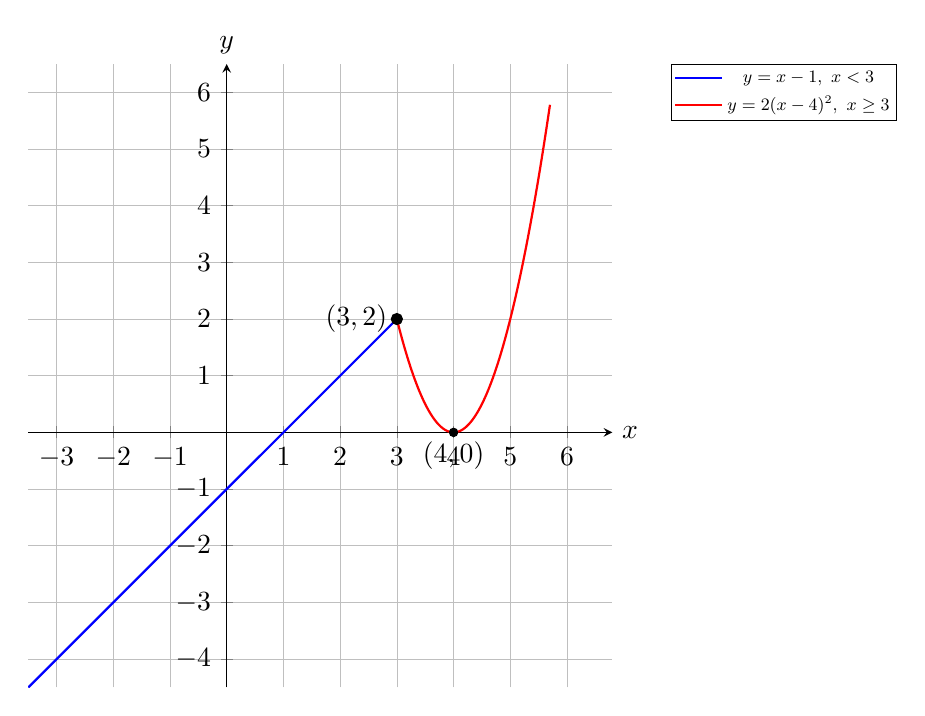
\begin{tikzpicture}
                            \begin{axis}[
        axis lines = middle,
        xlabel = $x$,
        ylabel = {$y$},
        xtick={-3,-2,...,6},
        ytick={-4,-3,...,6},
        xmin=-3.5, xmax=6.8,
        ymin=-4.5, ymax=6.5,
        width=9cm,
        height=9.5cm,
        grid=both,
        grid style={line width=.1pt, draw=gray!10},
        major grid style={line width=.2pt,draw=gray!50},
        x label style={anchor=west}, % label x ke kanan
        y label style={anchor=south}, % label y ke atas
        samples=200,
        legend style={
                at={(1.1,1)},
                anchor=north west,
                font=\small,         % mengecilkan ukuran font
                row sep=1pt,         % jarak antar baris legend
                inner sep=1pt,       % margin dalam kotak legend
                nodes={scale=0.7}    % skalakan isi legend
            }
    ]
\addplot[domain=-3.5:3, color=blue, thick] {x-1};
\addlegendentry{$y=x-1,\ x<3$}
\addplot[domain=3:5.7, color=red, thick] {2*(x-4)^2};
\addlegendentry{$y=2(x-4)^2,\ x\geq 3$}
\draw[fill=black] (3,2) circle (2pt) node[left] {$(3,2)$};
\draw[fill=black] (4,0) circle (1.5pt) node[below] {$(4,0)$};
\end{axis}
                        \end{tikzpicture}
                    \end{center}
                \end{enumerate}
            }
            \end{jawab}
            \item Diberikan $f(x)=\frac{x^3-1}{x-1}$.
            \begin{enumerate}
                \item Tentukan $\displaystyle\lim_{x\to 1}f(x)$.
                \item Buatlah sketsa grafik $y=f(x)$.
            \end{enumerate}
            \begin{jawab}[limit fungsi, faktorisasi, sketsa grafik]{
                \begin{enumerate}
                    \item Diperhatikan bahwa jika kita substitusi $x=1$ ke dalam $f(x)$, maka diperoleh bentuk tak tentu $\frac{0}{0}$. Oleh karena itu, kita faktorkan pembilangnya:
                    \begin{align*}
                        \colorlet{oldcolor}{.}
        \color{blue}
        \setlength{\fboxrule}{1pt} \boxed{\color{oldcolor}x^3-1 = (x-1)(x^2+x+1)}\color{oldcolor}.
                    \end{align*}
                    Dengan demikian, fungsi dapat disederhanakan menjadi
                    \begin{align*}
                        f(x) = \frac{x^3-1}{x-1} = \frac{(x-1)(x^2+x+1)}{x-1} = x^2+x+1, \quad x\neq 1.
                    \end{align*}
                    Sehingga limitnya adalah
                    \begin{align*}
                        \lim_{x\to 1}f(x) = \lim_{x\to 1}(x^2+x+1)= 1^2 + 1 + 1= 3.
                    \end{align*}
                    Jadi $\colorlet{oldcolor}{.}
        \color{red}
        \setlength{\fboxrule}{1pt} \boxed{\color{oldcolor}\lim_{x\to 1}f(x) = 3}\color{oldcolor}$.
                    \item Dari (a), grafik $y=f(x)$ sama dengan grafik parabola $y=x^2+x+1=\left(x+\frac{1}{2}\right)^2+\frac{3}{4}$ yang terbuka ke atas dengan titik puncak $\left(-\frac{1}{2},\frac{3}{4}\right)$, tetapi titik $(1,3)$ tidak termasuk dalam grafik (berlubang) karena $f(1)$ tidak terdefinisi. Sketsa grafik dari $y=f(x)$ adalah sebagai berikut:
                    \begin{center}
                        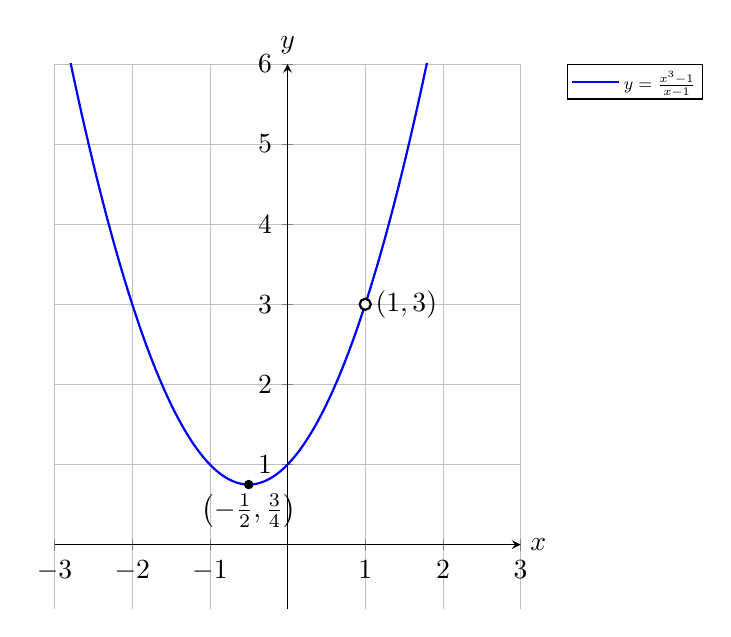
\begin{tikzpicture}
                            \begin{axis}[
        axis lines = middle,
        xlabel = $x$,
        ylabel = {$y$},
        xtick={-3,-2,...,3},
        ytick={0,1,...,6},
        xmin=-3, xmax=3,
        ymin=-0.8, ymax=6,
        width=7.5cm,
        height=8.5cm,
        grid=both,
        grid style={line width=.1pt, draw=gray!10},
        major grid style={line width=.2pt,draw=gray!50},
        x label style={anchor=west}, % label x ke kanan
        y label style={anchor=south}, % label y ke atas
        samples=200,
        legend style={
                at={(1.1,1)},
                anchor=north west,
                font=\small,         % mengecilkan ukuran font
                row sep=1pt,         % jarak antar baris legend
                inner sep=1pt,       % margin dalam kotak legend
                nodes={scale=0.7}    % skalakan isi legend
            }
    ]
\addplot[domain=-2.8:1.85, color=blue, thick] {x^2+x+1};
\addlegendentry{$y=\frac{x^3-1}{x-1}$}
\draw[fill=white, thick] (1,3) circle (2pt) node[right] {$(1,3)$};
\draw[fill=black] (-0.5,0.75) circle (1.5pt) node[below] {$\left(-\frac{1}{2},\frac{3}{4}\right)$};
\end{axis}
                        \end{tikzpicture}
                    \end{center}
                \end{enumerate}
            }
            \end{jawab}
            \item Diketahui kurva $x^2y+4x-3y^2=2$.
            \begin{enumerate}
                \item Dapatkan $\frac{dy}{dx}$ dengan menggunakan turunan fungsi implisit.
                \item Dari (a) dapatkan persamaan garis singgung pada kurva tersebut di titik $(1,1)$.
            \end{enumerate}
            \begin{jawab}[turunan implisit, aturan perkalian, persamaan garis singgung]{
                \begin{enumerate}
                    \item Kita turunkan kedua ruas persamaan $x^2y+4x-3y^2=2$ terhadap $x$, dengan mengingat bahwa $y$ adalah fungsi dari $x$ (yaitu $y=y(x)$). Dengan aturan perkalian, $\colorlet{oldcolor}{.}
        \color{blue}
        \setlength{\fboxrule}{1pt} \boxed{\color{oldcolor}\frac{d}{dx}(x^2y) = 2xy + x^2\frac{dy}{dx}}\color{oldcolor}$, dan dengan aturan rantai, $\colorlet{oldcolor}{.}
        \color{blue}
        \setlength{\fboxrule}{1pt} \boxed{\color{oldcolor}\frac{d}{dx}(3y^2) = 6y\frac{dy}{dx}}\color{oldcolor}$. Diperoleh
                    \begin{align*}
                        \frac{d}{dx}(x^2y) + \frac{d}{dx}(4x) - \frac{d}{dx}(3y^2) &= \frac{d}{dx}(2)\\
                        2xy + x^2\frac{dy}{dx} + 4 - 6y\frac{dy}{dx} &= 0.
                    \end{align*}
                    Selanjutnya, kumpulkan semua suku yang mengandung $\frac{dy}{dx}$ di satu ruas:
                    \begin{align*}
                        x^2\frac{dy}{dx} - 6y\frac{dy}{dx} &= -2xy - 4\\
                        (x^2 - 6y)\frac{dy}{dx} &= -2xy - 4\\
                        \frac{dy}{dx} &= \frac{-2xy - 4}{x^2 - 6y}.
                    \end{align*}
                    Jadi diperoleh $\colorlet{oldcolor}{.}
        \color{red}
        \setlength{\fboxrule}{1pt} \boxed{\color{oldcolor}\frac{dy}{dx} = \frac{-2xy - 4}{x^2 - 6y}}\color{oldcolor}$.
                    \item Terlebih dahulu dicek bahwa titik $(1,1)$ terletak pada kurva, yaitu $1^2(1)+4(1)-3(1)^2=1+4-3=2$. Untuk mendapatkan gradien garis singgung di titik $(1,1)$, substitusi $x=1$ dan $y=1$ ke dalam turunan yang telah diperoleh:
                    \begin{align*}
                        m=\left.\frac{dy}{dx}\right|_{(1,1)} = \frac{-2(1)(1) - 4}{(1)^2 - 6(1)}= \frac{-6}{-5}= \colorlet{oldcolor}{.}
        \color{blue}
        \setlength{\fboxrule}{1pt} \boxed{\color{oldcolor}\frac{6}{5}}\color{oldcolor}.
                    \end{align*}
                    Dengan menggunakan persamaan garis $y - y_1 = m(x - x_1)$, di mana $(x_1,y_1)=(1,1)$ dan $m=\frac{6}{5}$, diperoleh:
                    \begin{align*}
                        y - 1 &= \frac{6}{5}(x - 1)\\
                        y &= \frac{6}{5}x - \frac{6}{5} + \frac{5}{5}\\
                        y &= \frac{6}{5}x - \frac{1}{5}.
                    \end{align*}
                    Jadi persamaan garis singgung di titik $(1,1)$ adalah $\colorlet{oldcolor}{.}
        \color{red}
        \setlength{\fboxrule}{1pt} \boxed{\color{oldcolor}y = \frac{6}{5}x - \frac{1}{5}}\color{oldcolor}$ atau $6x-5y=1$.
                \end{enumerate}
            }
            \end{jawab}
        \end{enumerate}
\newpage
 \begin{center}
	{\underline{\textbf{\MakeUppercase{Soal dan Pembahasan ETS Kalkulus 1 Tahun 2025/2026}}}}
    \end{center}

    \begin{center}
	\begin{tabular}{lcl}
		Mata kuliah/SKS & : & Kalkulus 1 ( SM234101 ) / 3 SKS\\
		Hari, Tanggal & : & Selasa, 14 Oktober 2025\\
		Waktu & : & 07.00 - 08.40 / 100 menit\\
		Sifat & : & Tertutup\\
		Kelas & : & 113 dan 114\\
  ~
	\end{tabular}

    \noindent\rule{\textwidth}{2.pt}
        \end{center}
        \begin{enumerate}
            \item Dapatkan penyelesaian dari pertidaksamaan
            \begin{align*}
                \frac{x^2-x-12}{x^2+3x-10}\geq 0.
            \end{align*}
            \begin{jawab}[pertidaksamaan rasional, faktorisasi, garis bilangan, notasi interval]{~\\
                Karena ruas kanan pertidaksamaan sudah bernilai nol, maka kita bisa langsung memfaktorkan pembilang dan penyebut di ruas kiri. Diperoleh
                \begin{align*}
                    \frac{x^2-x-12}{x^2+3x-10} = \frac{(x-4)(x+3)}{(x+5)(x-2)} \geq 0.
                \end{align*}
                Selanjutnya, kita tentukan pembuat nol dari faktor-faktor tersebut, yaitu
                \begin{align*}
                    x-4 = 0 \quad &\vee\quad x+3 = 0 \quad \vee\quad x+5 = 0 \quad \vee\quad x-2 = 0\\
                    \colorlet{oldcolor}{.}
        \color{blue}
        \setlength{\fboxrule}{1pt} \boxed{\color{oldcolor}x=4}\color{oldcolor} \quad &\vee\quad \colorlet{oldcolor}{.}
        \color{blue}
        \setlength{\fboxrule}{1pt} \boxed{\color{oldcolor}x=-3}\color{oldcolor} \quad \vee\quad \colorlet{oldcolor}{.}
        \color{blue}
        \setlength{\fboxrule}{1pt} \boxed{\color{oldcolor}x=-5}\color{oldcolor} \quad \vee\quad \colorlet{oldcolor}{.}
        \color{blue}
        \setlength{\fboxrule}{1pt} \boxed{\color{oldcolor}x=2}\color{oldcolor}
                \end{align*}
                Selanjutnya, dibuat garis bilangan dan dilakukan uji titik pada ekspresi \(\frac{(x-4)(x+3)}{(x+5)(x-2)}\) sebagai berikut
                \begin{itemize}
                    \item Untuk \(x < -5\), misalkan \(x = -6\):
                    \[
                    \frac{(-6-4)(-6+3)}{(-6+5)(-6-2)} = \frac{(-10)(-3)}{(-1)(-8)} = \frac{30}{8} > 0
                    \]
                    \item Untuk \(-5 < x < -3\), misalkan \(x = -4\):
                    \[
                    \frac{(-4-4)(-4+3)}{(-4+5)(-4-2)} = \frac{(-8)(-1)}{(1)(-6)} = \frac{8}{-6} < 0
                    \]
                    \item Untuk \(-3 < x < 2\), misalkan \(x = 0\):
                    \[
                    \frac{(0-4)(0+3)}{(0+5)(0-2)} = \frac{(-4)(3)}{(5)(-2)} = \frac{-12}{-10} > 0
                    \]
                    \item Untuk \(2 < x < 4\), misalkan \(x = 3\):
                    \[
                    \frac{(3-4)(3+3)}{(3+5)(3-2)} = \frac{(-1)(6)}{(8)(1)} = \frac{-6}{8} < 0
                    \]
                    \item Untuk \(x > 4\), misalkan \(x = 5\):
                    \[
                    \frac{(5-4)(5+3)}{(5+5)(5-2)} = \frac{(1)(8)}{(10)(3)} = \frac{8}{30} > 0
                    \]
                \end{itemize}
                \begin{center}
                    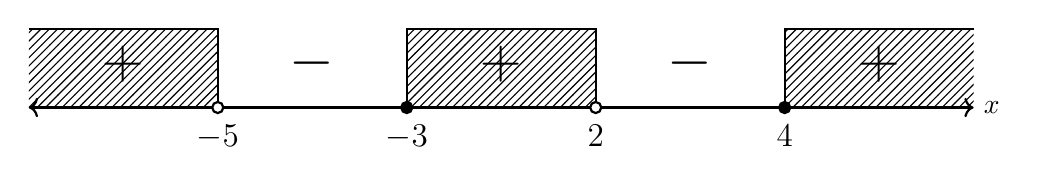
\begin{tikzpicture}
    \draw[thick,<->] (-6,0) -- (6,0) node[right] {$x$};
    \fill[pattern=north east lines] (-6,0) rectangle (-3.6,1);
    \fill[pattern=north east lines] (-1.2,0) rectangle (1.2,1);
    \fill[pattern=north east lines] (3.6,0) rectangle (6,1);
    \draw[thick] (-6,1) -- (-3.6,1) -- (-3.6,0);
    \draw[thick] (-1.2,0) -- (-1.2,1) -- (1.2,1) -- (1.2,0);
    \draw[thick] (3.6,0) -- (3.6,1) -- (6,1);
    \draw (-3.6,-0.1) node[below] {\large{$-5$}};
    \draw (-1.2,-0.1) node[below] {\large{$-3$}};
    \draw (1.2,-0.1) node[below] {\large{$2$}};
    \draw (3.6,-0.1) node[below] {\large{$4$}};
    \draw (-4.8,0.2) node[above] {\huge{$+$}};
    \draw (-2.4,0.2) node[above] {\huge{$-$}};
    \draw (0,0.2) node[above] {\huge{$+$}};
    \draw (2.4,0.2) node[above] {\huge{$-$}};
    \draw (4.8,0.2) node[above] {\huge{$+$}};
    \draw[fill=white, thick] (-3.6,0) circle (2pt);
    \draw[fill=black, thick] (-1.2,0) circle (2pt);
    \draw[fill=white, thick] (1.2,0) circle (2pt);
    \draw[fill=black, thick] (3.6,0) circle (2pt);
                    \end{tikzpicture}
                \end{center}
                Karena yang diminta adalah nilai yang lebih dari atau sama dengan nol, diambil interval yang bertanda positif beserta pembuat nol dari pembilang ($x=-3$ dan $x=4$). Pembuat nol dari penyebut ($x=-5$ dan $x=2$) tidak diikutkan karena membuat ekspresi tidak terdefinisi. Jadi penyelesaian dari pertidaksamaan tersebut adalah $\colorlet{oldcolor}{.}
        \color{red}
        \setlength{\fboxrule}{1pt} \boxed{\color{oldcolor}(-\infty, -5) \cup [-3, 2) \cup [4, \infty)}\color{oldcolor}$.
            }
            \end{jawab}
            \item \begin{enumerate}
                \item Dapatkan kemiringan garis $\ell$ yang melalui titik $(0,0)$ dan $(-2,1)$.
                \item Jika garis $\ell$ tegak lurus dengan garis yang menyinggung lingkaran yang berpusat di $(0,0)$ dan berjari-jari $\sqrt{5}$, di titik $(-2,1)$, maka dapatkan persamaan garis singgung lingkaran tersebut dan sketsalah.
            \end{enumerate}
            \begin{jawab}[kemiringan garis, garis tegak lurus, garis singgung lingkaran]{
                \begin{enumerate}
                    \item Kemiringan garis yang melalui dua titik $(x_1,y_1)$ dan $(x_2,y_2)$ adalah
                    \begin{align*}
                        m = \frac{y_2 - y_1}{x_2 - x_1}.
                    \end{align*}
                    Dengan substitusi $(x_1,y_1)=(0,0)$ dan $(x_2,y_2)=(-2,1)$, diperoleh
                    \begin{align*}
                        m_\ell = \frac{1 - 0}{-2 - 0} = \frac{1}{-2} = -\frac{1}{2}.
                    \end{align*}
                    Jadi kemiringan garis $\ell$ adalah $\colorlet{oldcolor}{.}
        \color{red}
        \setlength{\fboxrule}{1pt} \boxed{\color{oldcolor}m_\ell = -\frac{1}{2}}\color{oldcolor}$.
                    \item Persamaan lingkaran yang berpusat di $(0,0)$ dan berjari-jari $\sqrt{5}$ adalah $x^2 + y^2 = 5$. Diperhatikan bahwa titik $(-2,1)$ terletak pada lingkaran, karena $(-2)^2 + 1^2 = 4 + 1 = 5$. \\
                    Ingat kembali bahwa dua garis dengan gradien $m_1$ dan $m_2$ saling tegak lurus jika $\colorlet{oldcolor}{.}
        \color{blue}
        \setlength{\fboxrule}{1pt} \boxed{\color{oldcolor}m_1\cdot m_2=-1}\color{oldcolor}$. Karena garis singgung tegak lurus dengan garis $\ell$, maka gradien garis singgung $m_s$ memenuhi
                    \begin{align*}
                        m_\ell \cdot m_s = -1 \implies -\frac{1}{2}\cdot m_s = -1 \implies \colorlet{oldcolor}{.}
        \color{blue}
        \setlength{\fboxrule}{1pt} \boxed{\color{oldcolor}m_s = 2}\color{oldcolor}.
                    \end{align*}
                    Garis singgung melalui titik $(-2,1)$ dengan gradien $2$, sehingga dengan rumus $y - y_1 = m(x - x_1)$ diperoleh
                    \begin{align*}
                        y - 1 &= 2(x - (-2))\\
                        y - 1 &= 2x + 4\\
                        y &= 2x + 5.
                    \end{align*}
                    Jadi persamaan garis singgung lingkaran tersebut adalah $\colorlet{oldcolor}{.}
        \color{red}
        \setlength{\fboxrule}{1pt} \boxed{\color{oldcolor}y = 2x + 5}\color{oldcolor}$. Sketsa grafiknya adalah sebagai berikut:
                    \begin{center}
                        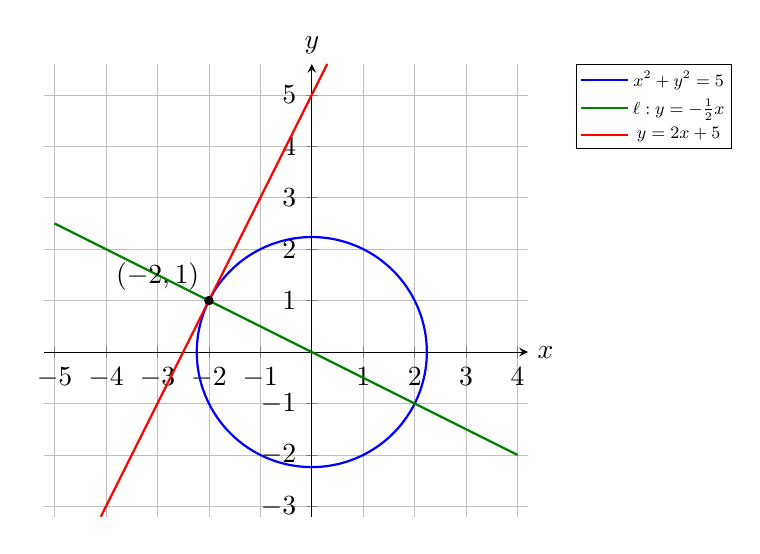
\begin{tikzpicture}
                            \begin{axis}[
        axis lines = middle,
        xlabel = $x$,
        ylabel = {$y$},
        xtick={-5,-4,...,4},
        ytick={-3,-2,...,5},
        xmin=-5.2, xmax=4.2,
        ymin=-3.2, ymax=5.6,
        axis equal image,
        width=8.5cm,
        grid=both,
        grid style={line width=.1pt, draw=gray!10},
        major grid style={line width=.2pt,draw=gray!50},
        x label style={anchor=west}, % label x ke kanan
        y label style={anchor=south}, % label y ke atas
        samples=200,
        legend style={
                at={(1.1,1)},
                anchor=north west,
                font=\small,         % mengecilkan ukuran font
                row sep=1pt,         % jarak antar baris legend
                inner sep=1pt,       % margin dalam kotak legend
                nodes={scale=0.7}    % skalakan isi legend
            }
    ]
\addplot[domain=0:360, color=blue, thick] ({sqrt(5)*cos(x)}, {sqrt(5)*sin(x)});
\addlegendentry{$x^2+y^2=5$}
\addplot[domain=-5:4, color=green!50!black, thick] {-x/2};
\addlegendentry{$\ell: y=-\frac{1}{2}x$}
\addplot[domain=-4.1:0.3, color=red, thick] {2*x+5};
\addlegendentry{$y=2x+5$}
\draw[fill=black] (-2,1) circle (1.5pt) node[above left] {$(-2,1)$};
\end{axis}
                        \end{tikzpicture}
                    \end{center}
                    \end{enumerate}
            }
                \end{jawab}
            \item Tuliskan rumus turunan dari $fg$ yaitu $\frac{d}{dx}(f(x)g(x))$\\
            Selanjutnya, dapatkan turunan dari $fg$, jika diketahui $f(x)=3x^2-7x$ dan $g(x)=3-2x^2$.
            \begin{jawab}[turunan, aturan perkalian]{~\\
                Ingat kembali aturan turunan untuk perkalian fungsi, yaitu
                \[
                \colorlet{oldcolor}{.}
        \color{red}
        \setlength{\fboxrule}{1pt} \boxed{\color{oldcolor}\frac{d}{dx}\left(f(x)g(x)\right) = f'(x)g(x) + f(x)g'(x)}\color{oldcolor}.
                \]
                Selanjutnya, kita hitung turunan dari \(f(x)\) dan \(g(x)\):
                \begin{align*}
                    \colorlet{oldcolor}{.}
        \color{blue}
        \setlength{\fboxrule}{1pt} \boxed{\color{oldcolor}f'(x) = \frac{d}{dx}(3x^2 - 7x) = 6x - 7}\color{oldcolor}\\
                    \colorlet{oldcolor}{.}
        \color{blue}
        \setlength{\fboxrule}{1pt} \boxed{\color{oldcolor}g'(x) = \frac{d}{dx}(3 - 2x^2) = -4x}\color{oldcolor}
                \end{align*}
                Dengan demikian, turunan dari \(fg\) adalah
                \begin{align*}
                    \frac{d}{dx}\left(f(x)g(x)\right) &= (6x - 7)(3 - 2x^2) + (3x^2 - 7x)(-4x)\\
                    &= (18x - 12x^3 - 21 + 14x^2) + (-12x^3 + 28x^2)\\
                    &= \colorlet{oldcolor}{.}
        \color{red}
        \setlength{\fboxrule}{1pt} \boxed{\color{oldcolor}-24x^3 + 42x^2 + 18x - 21}\color{oldcolor}.
                \end{align*}
            }
            \end{jawab}
            \item Dapatkan $\displaystyle \lim_{x\to 3} \frac{\sqrt{3x+7}-4}{x-3}$.
            \begin{jawab}[limit fungsi, bentuk tak tentu, perkalian sekawan]{~\\
                Diperhatikan bahwa jika kita substitusi $x=3$ secara langsung, diperoleh $\frac{\sqrt{16}-4}{0}=\frac{0}{0}$ yang merupakan bentuk tak tentu. Untuk menyelesaikan limit tersebut, kita kalikan dengan bentuk konjugat (sekawan) dari pembilangnya, sehingga diperoleh
                \begin{align*}
                    \lim_{x\to 3} \frac{\sqrt{3x+7}-4}{x-3} &= \lim_{x\to 3} \frac{\sqrt{3x+7}-4}{x-3}\cdot\frac{\sqrt{3x+7}+4}{\sqrt{3x+7}+4}\\
                    &= \lim_{x\to 3} \frac{3x+7-16}{(x-3)(\sqrt{3x+7}+4)}\\
                    &= \lim_{x\to 3} \frac{3(x-3)}{(x-3)(\sqrt{3x+7}+4)}\\
                    &= \lim_{x\to 3} \frac{3}{\sqrt{3x+7}+4}\\
                    &= \frac{3}{\sqrt{16}+4}\\
                    &= \colorlet{oldcolor}{.}
        \color{red}
        \setlength{\fboxrule}{1pt} \boxed{\color{oldcolor}\frac{3}{8}}\color{oldcolor}.
                \end{align*}
            }
            \end{jawab}
            \item Diberikan fungsi $f(x)=\frac{1}{x-1}$ dan $g(x)=x^2$.
            \begin{enumerate}
                \item Dapatkan $(f\circ g)(x)$.
                \item Jika diketahui $(p\circ g)(x)=  x^2-3$, dapatkan $p(x)$.
            \end{enumerate}
            \begin{jawab}[fungsi komposisi]{
                \begin{enumerate}
                    \item Diperhatikan bahwa
                    \begin{align*}
                        (f\circ g)(x) = f(g(x)) = f(x^2) = \colorlet{oldcolor}{.}
        \color{red}
        \setlength{\fboxrule}{1pt} \boxed{\color{oldcolor}\frac{1}{x^2-1}}\color{oldcolor},
                    \end{align*}
                    dengan domain $\{x\in\mathbb{R}: x^2\neq 1\}=\mathbb{R}\setminus\{-1,1\}$.
                    \item Diperhatikan bahwa $(p\circ g)(x) = p(g(x)) = p(x^2) = x^2-3$. Misalkan $\colorlet{oldcolor}{.}
        \color{blue}
        \setlength{\fboxrule}{1pt} \boxed{\color{oldcolor}u = x^2}\color{oldcolor}$, maka diperoleh
                    \begin{align*}
                        p(u) = u - 3.
                    \end{align*}
                    Dengan mengganti $u$ dengan $x$, didapatkan $\colorlet{oldcolor}{.}
        \color{red}
        \setlength{\fboxrule}{1pt} \boxed{\color{oldcolor}p(x) = x - 3}\color{oldcolor}$.\\
                    Sebagai pengecekan, $(p\circ g)(x) = p(x^2) = x^2 - 3$, sesuai dengan yang diketahui.
                \end{enumerate}
            }
            \end{jawab}
        \end{enumerate}

\newpage
 \begin{center}
	{\underline{\textbf{\MakeUppercase{Soal dan Pembahasan ETS Kalkulus 1 Tahun 2025/2026}}}}
    \end{center}

    \begin{center}
	\begin{tabular}{lcl}
		Course / Credit & : & Kalkulus 1 ( SM234101 ) / 3 SKS\\
		Day, Date & : & Tuesday, 14 October 2025\\
		Time / Exam Time & : & 07.00 - 08.40 / 100 menit\\
		Type & : & Closed\\
		Class & : & 2, 3, 68, 69\\
  ~
	\end{tabular}

    \noindent\rule{\textwidth}{2.pt}
        \end{center}
        \begin{enumerate}
            \item Find the solution of the following inequality
            \begin{align*}
                \frac{x^2-x-12}{x^2+3x-10}\geq 0.
            \end{align*}
            \begin{jawab}[pertidaksamaan rasional, faktorisasi, garis bilangan, notasi interval]{~\\
                Soal ini sama dengan soal nomor 1 pada ujian kelas 113 dan 114. Dengan memfaktorkan pembilang dan penyebut, diperoleh
                \begin{align*}
                    \frac{(x-4)(x+3)}{(x+5)(x-2)} \geq 0,
                \end{align*}
                dengan pembuat nol $\colorlet{oldcolor}{.}
        \color{blue}
        \setlength{\fboxrule}{1pt} \boxed{\color{oldcolor}x=-5,~x=-3,~x=2,~x=4}\color{oldcolor}$. Dengan uji titik pada setiap interval (misalnya $x=-6,-4,0,3,5$), didapatkan tanda dari setiap interval sebagai berikut
                \begin{center}
                    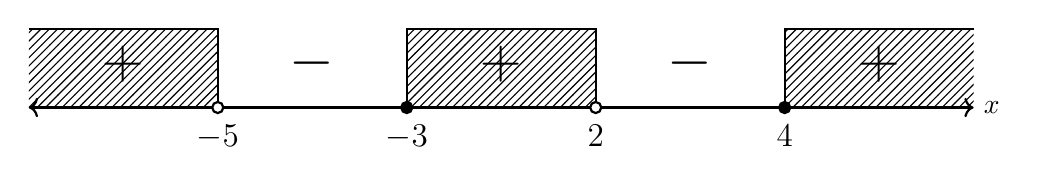
\begin{tikzpicture}
    \draw[thick,<->] (-6,0) -- (6,0) node[right] {$x$};
    \fill[pattern=north east lines] (-6,0) rectangle (-3.6,1);
    \fill[pattern=north east lines] (-1.2,0) rectangle (1.2,1);
    \fill[pattern=north east lines] (3.6,0) rectangle (6,1);
    \draw[thick] (-6,1) -- (-3.6,1) -- (-3.6,0);
    \draw[thick] (-1.2,0) -- (-1.2,1) -- (1.2,1) -- (1.2,0);
    \draw[thick] (3.6,0) -- (3.6,1) -- (6,1);
    \draw (-3.6,-0.1) node[below] {\large{$-5$}};
    \draw (-1.2,-0.1) node[below] {\large{$-3$}};
    \draw (1.2,-0.1) node[below] {\large{$2$}};
    \draw (3.6,-0.1) node[below] {\large{$4$}};
    \draw (-4.8,0.2) node[above] {\huge{$+$}};
    \draw (-2.4,0.2) node[above] {\huge{$-$}};
    \draw (0,0.2) node[above] {\huge{$+$}};
    \draw (2.4,0.2) node[above] {\huge{$-$}};
    \draw (4.8,0.2) node[above] {\huge{$+$}};
    \draw[fill=white, thick] (-3.6,0) circle (2pt);
    \draw[fill=black, thick] (-1.2,0) circle (2pt);
    \draw[fill=white, thick] (1.2,0) circle (2pt);
    \draw[fill=black, thick] (3.6,0) circle (2pt);
                    \end{tikzpicture}
                \end{center}
                Diambil interval yang bertanda positif beserta pembuat nol pembilang ($x=-3$ dan $x=4$), tanpa pembuat nol penyebut ($x=-5$ dan $x=2$). Jadi penyelesaiannya adalah $\colorlet{oldcolor}{.}
        \color{red}
        \setlength{\fboxrule}{1pt} \boxed{\color{oldcolor}(-\infty, -5) \cup [-3, 2) \cup [4, \infty)}\color{oldcolor}$.
            }
            \end{jawab}
            \item \begin{enumerate}
                \item Find the gradient of the line $\ell$ which goes through $(0,0)$ and $(-2,1)$.
                \item If line $\ell$ is perpendicular with the line that tangent with a circle centered at $(0,0)$ and radius $\sqrt{5}$, at $(-2,1)$, then find the aforementioned tangent line equation and sketch the graph.
            \end{enumerate}
            \begin{jawab}[kemiringan garis, garis tegak lurus, garis singgung lingkaran]{
                \begin{enumerate}
                    \item Dengan rumus kemiringan garis melalui dua titik, diperoleh
                    \begin{align*}
                        m_\ell = \frac{y_2 - y_1}{x_2 - x_1} = \frac{1 - 0}{-2 - 0} = \colorlet{oldcolor}{.}
        \color{red}
        \setlength{\fboxrule}{1pt} \boxed{\color{oldcolor}-\frac{1}{2}}\color{oldcolor}.
                    \end{align*}
                    \item Titik $(-2,1)$ terletak pada lingkaran $x^2+y^2=5$ karena $(-2)^2+1^2=5$. Karena garis singgung tegak lurus dengan $\ell$, maka $\colorlet{oldcolor}{.}
        \color{blue}
        \setlength{\fboxrule}{1pt} \boxed{\color{oldcolor}m_\ell\cdot m_s=-1}\color{oldcolor}$, sehingga $-\frac{1}{2}m_s=-1$ dan diperoleh $\colorlet{oldcolor}{.}
        \color{blue}
        \setlength{\fboxrule}{1pt} \boxed{\color{oldcolor}m_s = 2}\color{oldcolor}$. Garis singgung melalui titik $(-2,1)$, sehingga
                    \begin{align*}
                        y - 1 = 2(x + 2) \implies y = 2x + 5.
                    \end{align*}
                    Jadi persamaan garis singgungnya adalah $\colorlet{oldcolor}{.}
        \color{red}
        \setlength{\fboxrule}{1pt} \boxed{\color{oldcolor}y = 2x + 5}\color{oldcolor}$. Sketsa grafiknya adalah sebagai berikut:
                    \begin{center}
                        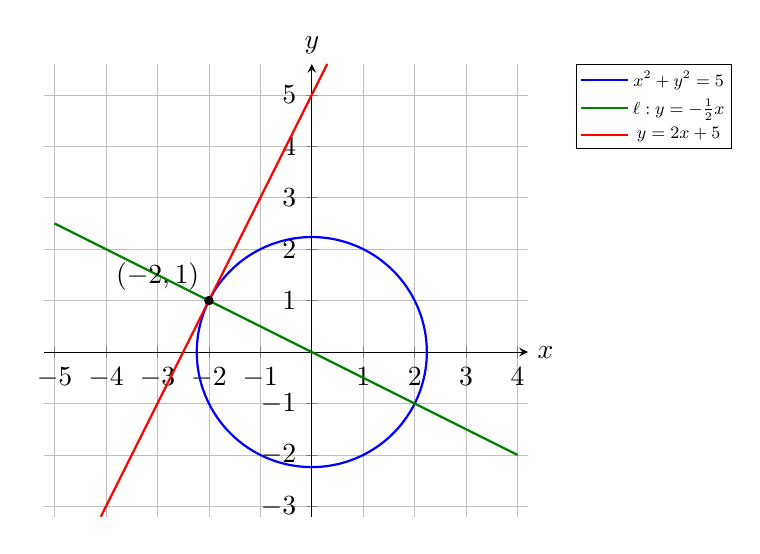
\begin{tikzpicture}
                            \begin{axis}[
        axis lines = middle,
        xlabel = $x$,
        ylabel = {$y$},
        xtick={-5,-4,...,4},
        ytick={-3,-2,...,5},
        xmin=-5.2, xmax=4.2,
        ymin=-3.2, ymax=5.6,
        axis equal image,
        width=8.5cm,
        grid=both,
        grid style={line width=.1pt, draw=gray!10},
        major grid style={line width=.2pt,draw=gray!50},
        x label style={anchor=west}, % label x ke kanan
        y label style={anchor=south}, % label y ke atas
        samples=200,
        legend style={
                at={(1.1,1)},
                anchor=north west,
                font=\small,         % mengecilkan ukuran font
                row sep=1pt,         % jarak antar baris legend
                inner sep=1pt,       % margin dalam kotak legend
                nodes={scale=0.7}    % skalakan isi legend
            }
    ]
\addplot[domain=0:360, color=blue, thick] ({sqrt(5)*cos(x)}, {sqrt(5)*sin(x)});
\addlegendentry{$x^2+y^2=5$}
\addplot[domain=-5:4, color=green!50!black, thick] {-x/2};
\addlegendentry{$\ell: y=-\frac{1}{2}x$}
\addplot[domain=-4.1:0.3, color=red, thick] {2*x+5};
\addlegendentry{$y=2x+5$}
\draw[fill=black] (-2,1) circle (1.5pt) node[above left] {$(-2,1)$};
\end{axis}
                        \end{tikzpicture}
                    \end{center}
                \end{enumerate}
            }
            \end{jawab}
            \item Write the derivative formula of $fg$ that is $\frac{d}{dx}(f(x)g(x))$\\
            Then, find the derivative of $fg$, given that $f(x)=3x^2-7x$ and $g(x)=3-2x^2$.
            \begin{jawab}[turunan, aturan perkalian]{~\\
                Ingat kembali aturan turunan untuk perkalian fungsi, yaitu
                \[
                \colorlet{oldcolor}{.}
        \color{red}
        \setlength{\fboxrule}{1pt} \boxed{\color{oldcolor}\frac{d}{dx}\left(f(x)g(x)\right) = f'(x)g(x) + f(x)g'(x)}\color{oldcolor}.
                \]
                Karena $\colorlet{oldcolor}{.}
        \color{blue}
        \setlength{\fboxrule}{1pt} \boxed{\color{oldcolor}f'(x) = 6x - 7}\color{oldcolor}$ dan $\colorlet{oldcolor}{.}
        \color{blue}
        \setlength{\fboxrule}{1pt} \boxed{\color{oldcolor}g'(x) = -4x}\color{oldcolor}$, diperoleh
                \begin{align*}
                    \frac{d}{dx}\left(f(x)g(x)\right) &= (6x - 7)(3 - 2x^2) + (3x^2 - 7x)(-4x)\\
                    &= (18x - 12x^3 - 21 + 14x^2) + (-12x^3 + 28x^2)\\
                    &= \colorlet{oldcolor}{.}
        \color{red}
        \setlength{\fboxrule}{1pt} \boxed{\color{oldcolor}-24x^3 + 42x^2 + 18x - 21}\color{oldcolor}.
                \end{align*}
            }
            \end{jawab}
            \item Calculate $\displaystyle \lim_{x\to 3} \frac{\sqrt{3x+7}-4}{x-3}$.
            \begin{jawab}[limit fungsi, bentuk tak tentu, perkalian sekawan]{~\\
                Substitusi langsung $x=3$ menghasilkan bentuk tak tentu $\frac{0}{0}$, sehingga kita kalikan dengan bentuk sekawan dari pembilangnya:
                \begin{align*}
                    \lim_{x\to 3} \frac{\sqrt{3x+7}-4}{x-3} &= \lim_{x\to 3} \frac{\sqrt{3x+7}-4}{x-3}\cdot\frac{\sqrt{3x+7}+4}{\sqrt{3x+7}+4}\\
                    &= \lim_{x\to 3} \frac{3(x-3)}{(x-3)(\sqrt{3x+7}+4)}\\
                    &= \lim_{x\to 3} \frac{3}{\sqrt{3x+7}+4}\\
                    &= \colorlet{oldcolor}{.}
        \color{red}
        \setlength{\fboxrule}{1pt} \boxed{\color{oldcolor}\frac{3}{8}}\color{oldcolor}.
                \end{align*}
            }
            \end{jawab}
            \item Given a function $f(x)=\frac{1}{x-1}$ and $g(x)=x^2$.
            \begin{enumerate}
                \item Find $(f\circ g)(x)$.
                \item Given $(p\circ g)(x)=  x^2-3$, then find $p(x)$.
            \end{enumerate}
            \begin{jawab}[fungsi komposisi]{
                \begin{enumerate}
                    \item Diperhatikan bahwa $(f\circ g)(x) = f(g(x)) = f(x^2) = \colorlet{oldcolor}{.}
        \color{red}
        \setlength{\fboxrule}{1pt} \boxed{\color{oldcolor}\frac{1}{x^2-1}}\color{oldcolor}$, dengan domain $\mathbb{R}\setminus\{-1,1\}$.
                    \item Diperhatikan bahwa $p(g(x)) = p(x^2) = x^2-3$. Dengan memisalkan $\colorlet{oldcolor}{.}
        \color{blue}
        \setlength{\fboxrule}{1pt} \boxed{\color{oldcolor}u = x^2}\color{oldcolor}$, diperoleh $p(u)=u-3$, sehingga $\colorlet{oldcolor}{.}
        \color{red}
        \setlength{\fboxrule}{1pt} \boxed{\color{oldcolor}p(x) = x - 3}\color{oldcolor}$.
                \end{enumerate}
            }
            \end{jawab}
        \end{enumerate}
               \newpage
 \begin{center}
	{\underline{\textbf{\MakeUppercase{Soal dan Pembahasan ETS Kalkulus 1 Tahun 2025/2026}}}}
    \end{center}

    \begin{center}
	\begin{tabular}{lcl}
		Mata kuliah/SKS & : & Kalkulus 1 ( SM234101 ) / 3 SKS\\
		Hari, Tanggal & : & Selasa, 14 Oktober 2025\\
		Waktu & : & 09.00 - 10.40 / 100 menit\\
		Sifat & : & Tertutup\\
		Kelas & : & 5-12, 23-29, 115 dan 116\\
  ~
	\end{tabular}

    \noindent\rule{\textwidth}{2.pt}
        \end{center}
        \begin{enumerate}
            \item Selesaikan pertidaksamaan berikut
            \begin{align*}
                \frac{1}{x+2} \leq \frac{2}{x-1}.
            \end{align*}
            \begin{jawab}[pertidaksamaan rasional, pecahan, garis bilangan, notasi interval]{~\\
                Untuk menyelesaikan pertidaksamaan rasional, pastikan ruas kanan sudah bernilai nol. Perlu diingat bahwa kita \textbf{tidak boleh} mengalikan silang karena tanda penyebut belum diketahui. Dengan mengurangkan \(\frac{2}{x-1}\) dari kedua ruas, didapatkan
                \begin{align*}
                    \frac{1}{x+2} - \frac{2}{x-1} &\leq 0\\
                    \frac{(x-1) - 2(x+2)}{(x+2)(x-1)} &\leq 0\\
                    \frac{-x-5}{(x+2)(x-1)} &\leq 0.
                \end{align*}
                Dengan mengalikan kedua ruas dengan $-1$ (tanda pertidaksamaan berbalik), diperoleh
                \begin{align}
                    \frac{x+5}{(x+2)(x-1)} \geq 0. \label{ineq:soal7}
                \end{align}
                Didapatkan pembuat nol dari faktor-faktornya adalah
                \begin{align*}
                    x+5 = 0 \quad &\vee\quad x+2 = 0 \quad \vee\quad x-1=0\\
                    \colorlet{oldcolor}{.}
        \color{blue}
        \setlength{\fboxrule}{1pt} \boxed{\color{oldcolor}x=-5}\color{oldcolor} \quad &\vee\quad \colorlet{oldcolor}{.}
        \color{blue}
        \setlength{\fboxrule}{1pt} \boxed{\color{oldcolor}x=-2}\color{oldcolor} \quad \vee\quad \colorlet{oldcolor}{.}
        \color{blue}
        \setlength{\fboxrule}{1pt} \boxed{\color{oldcolor}x=1}\color{oldcolor}
                \end{align*}
                Selanjutnya, dibuat garis bilangan dan dilakukan uji titik pada ekspresi \eqref{ineq:soal7} sebagai berikut
                \begin{itemize}
                    \item Untuk \(x < -5\), misalkan \(x = -6\):
                    \(
                    \frac{-6+5}{(-6+2)(-6-1)} = \frac{-1}{(-4)(-7)} = \frac{-1}{28} < 0
                    \)
                    \item Untuk \(-5 < x < -2\), misalkan \(x = -3\):
                    \(
                    \frac{-3+5}{(-3+2)(-3-1)} = \frac{2}{(-1)(-4)} = \frac{2}{4} > 0
                    \)
                    \item Untuk \(-2 < x < 1\), misalkan \(x = 0\):
                    \(
                    \frac{0+5}{(0+2)(0-1)} = \frac{5}{-2} < 0
                    \)
                    \item Untuk \(x > 1\), misalkan \(x = 2\):
                    \(
                    \frac{2+5}{(2+2)(2-1)} = \frac{7}{4} > 0
                    \)
                \end{itemize}
                \begin{center}
                    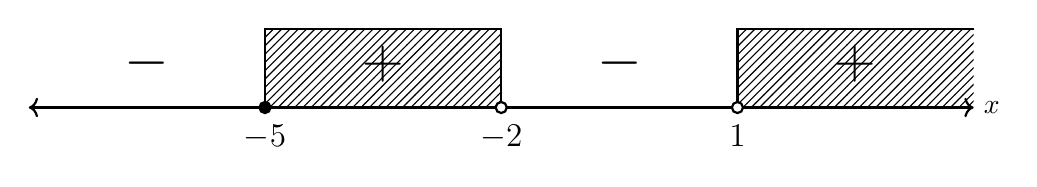
\begin{tikzpicture}
    \draw[thick,<->] (-6,0) -- (6,0) node[right] {$x$};
    \fill[pattern=north east lines] (-3,0) rectangle (0,1);
    \fill[pattern=north east lines] (3,0) rectangle (6,1);
    \draw[thick] (-3,0) -- (-3,1) -- (0,1) -- (0,0);
    \draw[thick] (3,0) -- (3,1) -- (6,1);
    \draw (-3,-0.1) node[below] {\large{$-5$}};
    \draw (0,-0.1) node[below] {\large{$-2$}};
    \draw (3,-0.1) node[below] {\large{$1$}};
    \draw (-4.5,0.2) node[above] {\huge{$-$}};
    \draw (-1.5,0.2) node[above] {\huge{$+$}};
    \draw (1.5,0.2) node[above] {\huge{$-$}};
    \draw (4.5,0.2) node[above] {\huge{$+$}};
    \draw[fill=black, thick] (-3,0) circle (2pt);
    \draw[fill=white, thick] (0,0) circle (2pt);
    \draw[fill=white, thick] (3,0) circle (2pt);
                    \end{tikzpicture}
                \end{center}
                Karena yang diminta adalah nilai \(x\) yang membuat ekspresi \eqref{ineq:soal7} lebih dari atau sama dengan nol, diambil interval bertanda positif beserta pembuat nol pembilang ($x=-5$), tanpa pembuat nol penyebut ($x=-2$ dan $x=1$). Jadi solusi dari pertidaksamaan tersebut adalah $-5\leq x<-2$ atau $x>1$. Dalam notasi interval, solusi tersebut dapat ditulis sebagai $\colorlet{oldcolor}{.}
        \color{red}
        \setlength{\fboxrule}{1pt} \boxed{\color{oldcolor}[-5, -2) \cup (1, \infty)}\color{oldcolor}$.
            }
            \end{jawab}
            \item Gambarkan kurva dasar $y=\frac{1}{x}$. Berdasarkan kurva dasar tersebut, gunakan translasi (pergeseran) untuk menggambar kurva $y=\frac{1}{x-2}+4$ (Jelaskan ilustrasinya).
            \begin{jawab}[fungsi rasional, asimtot, translasi grafik]{~\\
                Kurva dasar $y=\frac{1}{x}$ merupakan hiperbola dengan asimtot tegak $x=0$ (sumbu-$y$) dan asimtot datar $y=0$ (sumbu-$x$), serta grafiknya berada di kuadran I dan III. Sketsa kurva dasarnya adalah sebagai berikut.
                \begin{center}
                    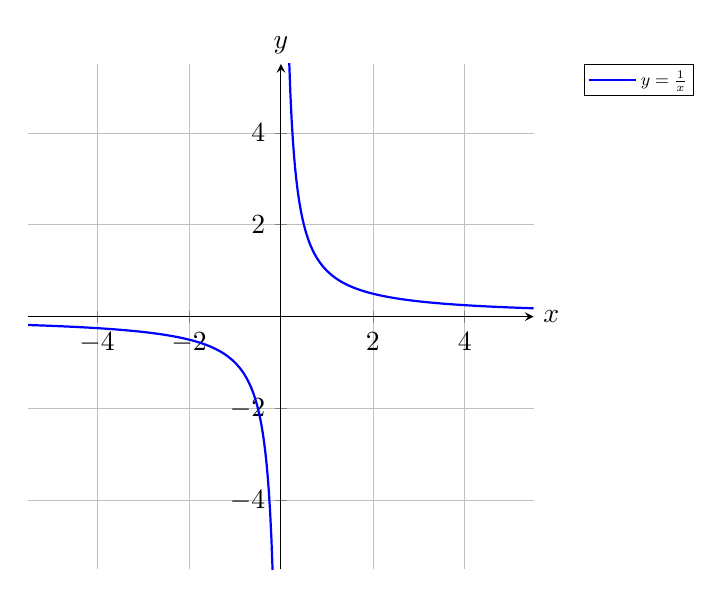
\begin{tikzpicture}
                        \begin{axis}[
        axis lines = middle,
        xlabel = $x$,
        ylabel = {$y$},
        xtick={-4,-2,...,4},
        ytick={-4,-2,...,4},
        xmin=-5.5, xmax=5.5,
        ymin=-5.5, ymax=5.5,
        width=8cm,
        height=8cm,
        grid=both,
        grid style={line width=.1pt, draw=gray!10},
        major grid style={line width=.2pt,draw=gray!50},
        x label style={anchor=west}, % label x ke kanan
        y label style={anchor=south}, % label y ke atas
        samples=200,
        legend style={
                at={(1.1,1)},
                anchor=north west,
                font=\small,         % mengecilkan ukuran font
                row sep=1pt,         % jarak antar baris legend
                inner sep=1pt,       % margin dalam kotak legend
                nodes={scale=0.7}    % skalakan isi legend
            }
    ]
\addplot[domain=-5.5:-0.18, color=blue, thick] {1/x};
\addlegendentry{$y=\frac{1}{x}$}
\addplot[domain=0.18:5.5, color=blue, thick, forget plot] {1/x};
\end{axis}
                    \end{tikzpicture}
                \end{center}
                Ingat kembali bahwa mengganti $x$ dengan $x-2$ berarti menggeser grafik sejauh $2$ satuan ke kanan, dan menambahkan konstanta $4$ berarti menggeser grafik sejauh $4$ satuan ke atas. Dengan demikian, proses translasinya adalah sebagai berikut.
                \begin{enumerate}
                    \item[(i)] Geser kurva $y=\frac{1}{x}$ sejauh $2$ satuan ke kanan, sehingga diperoleh kurva $y=\frac{1}{x-2}$ dengan asimtot tegak $x=2$ dan asimtot datar $y=0$.
                    \item[(ii)] Geser kurva $y=\frac{1}{x-2}$ sejauh $4$ satuan ke atas, sehingga diperoleh kurva $y=\frac{1}{x-2}+4$ dengan $\colorlet{oldcolor}{.}
        \color{blue}
        \setlength{\fboxrule}{1pt} \boxed{\color{oldcolor}\text{asimtot tegak } x=2 \text{ dan asimtot datar } y=4}\color{oldcolor}$.
                \end{enumerate}
                Dengan kata lain, titik pusat hiperbola berpindah dari $(0,0)$ ke $(2,4)$. Sebagai bantuan, titik potong dengan sumbu-$y$ ($x=0$) adalah $y=-\frac{1}{2}+4=\frac{7}{2}$, dan titik potong dengan sumbu-$x$ ($y=0$) adalah $\frac{1}{x-2}=-4$, yaitu $x=\frac{7}{4}$. Sketsa kurvanya adalah sebagai berikut.
                \begin{center}
                    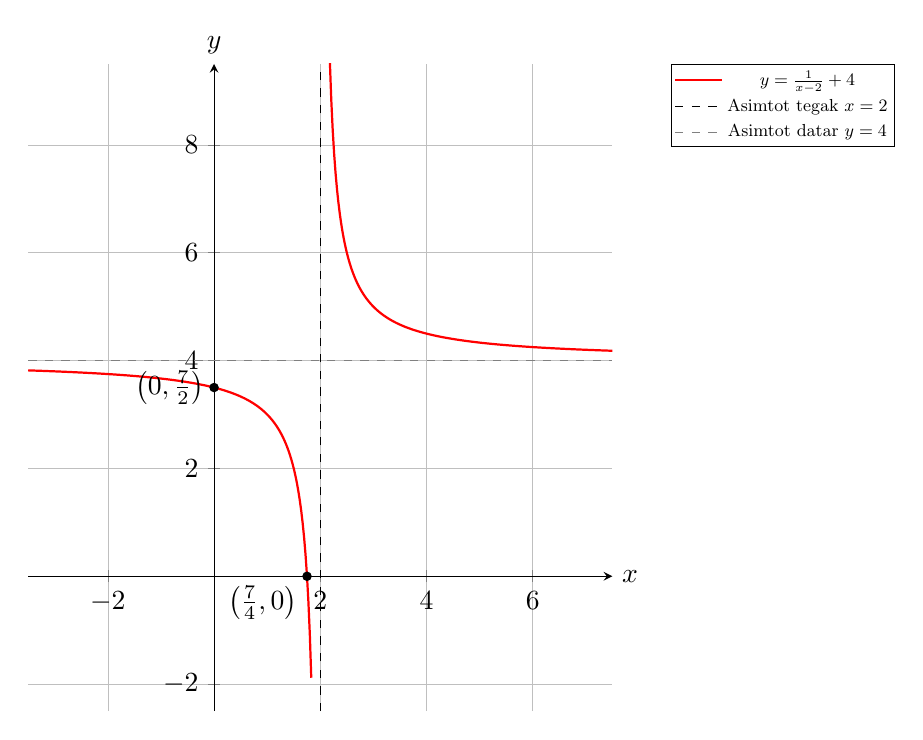
\begin{tikzpicture}
                        \begin{axis}[
        axis lines = middle,
        xlabel = $x$,
        ylabel = {$y$},
        xtick={-2,0,...,6},
        ytick={-2,0,...,8},
        xmin=-3.5, xmax=7.5,
        ymin=-2.5, ymax=9.5,
        width=9cm,
        height=9.8cm,
        grid=both,
        grid style={line width=.1pt, draw=gray!10},
        major grid style={line width=.2pt,draw=gray!50},
        x label style={anchor=west}, % label x ke kanan
        y label style={anchor=south}, % label y ke atas
        samples=200,
        legend style={
                at={(1.1,1)},
                anchor=north west,
                font=\small,         % mengecilkan ukuran font
                row sep=1pt,         % jarak antar baris legend
                inner sep=1pt,       % margin dalam kotak legend
                nodes={scale=0.7}    % skalakan isi legend
            }
    ]
\addplot[domain=-3.5:1.83, color=red, thick] {1/(x-2)+4};
\addlegendentry{$y=\frac{1}{x-2}+4$}
\addplot[domain=2.18:7.5, color=red, thick, forget plot] {1/(x-2)+4};
\addplot[color=black, dashed] coordinates {(2,-2.5) (2,9.5)};
\addlegendentry{Asimtot tegak $x=2$}
\addplot[domain=-3.5:7.5, color=gray, dashed, samples=2] {4};
\addlegendentry{Asimtot datar $y=4$}
\draw[fill=black] (0,3.5) circle (1.5pt) node[left] {$\left(0,\frac{7}{2}\right)$};
\draw[fill=black] (1.75,0) circle (1.5pt) node[below left] {$\left(\frac{7}{4},0\right)$};
\end{axis}
                    \end{tikzpicture}
                \end{center}
            }
            \end{jawab}
            \item Diberikan fungsi $f(x)=\frac{1}{x-2}$ dan $g(x)=\sqrt{5-x}$. Tentukan :
            \begin{enumerate}
                \item Domain fungsi $f$ dan $g$.
                \item Fungsi $(f\circ g)(x)$ dan $\left(\frac{f}{g}\right) (x)$ beserta domainnya masing-masing.
            \end{enumerate}
            \begin{jawab}[domain fungsi, fungsi komposisi, operasi fungsi]{
                \begin{enumerate}
                    \item Diperhatikan bahwa $f(x)$ merupakan fungsi rasional, sehingga domainnya adalah semua bilangan real kecuali nilai yang membuat penyebutnya sama dengan nol, yaitu $x-2\neq 0$. Jadi
                    \[
                    \colorlet{oldcolor}{.}
        \color{red}
        \setlength{\fboxrule}{1pt} \boxed{\color{oldcolor}D(f)=\{x \in \mathbb{R} : x \neq 2\}}\color{oldcolor}.
                    \]
                    Selanjutnya, diperhatikan bahwa $g(x)$ memuat akar kuadrat, sehingga domainnya adalah semua bilangan real yang membuat ekspresi di dalam akar kuadrat tak negatif, yaitu $5-x\geq 0$ atau $x\leq 5$. Jadi
                    \[
                    \colorlet{oldcolor}{.}
        \color{red}
        \setlength{\fboxrule}{1pt} \boxed{\color{oldcolor}D(g)=\{x \in \mathbb{R} : x \leq 5\} = (-\infty,5]}\color{oldcolor}.
                    \]
                    \item Diperhatikan bahwa
                    \begin{align*}
                        (f\circ g)(x) = f(g(x)) = f(\sqrt{5-x}) = \colorlet{oldcolor}{.}
        \color{red}
        \setlength{\fboxrule}{1pt} \boxed{\color{oldcolor}\frac{1}{\sqrt{5-x} - 2}}\color{oldcolor}
                    \end{align*}
                    Domain dari fungsi komposisi $f\circ g$ adalah semua nilai $x$ pada domain $g$ sehingga nilai dari $g(x)$ berada pada domain $f$, yaitu
                    \begin{align*}
                        \colorlet{oldcolor}{.}
        \color{blue}
        \setlength{\fboxrule}{1pt} \boxed{\color{oldcolor}D(f\circ g) = \{x \in D(g) : g(x) \in D(f)\} = \{x \in (-\infty, 5] : \sqrt{5-x} \neq 2\}}\color{oldcolor}.
                    \end{align*}
                    Karena $\sqrt{5-x} = 2$ jika dan hanya jika $5-x = 4$, yang berarti $x = 1$, didapatkan
                    \begin{align*}
                        \colorlet{oldcolor}{.}
        \color{red}
        \setlength{\fboxrule}{1pt} \boxed{\color{oldcolor}D(f\circ g) = (-\infty, 5] \setminus \{1\} = (-\infty, 1) \cup (1, 5]}\color{oldcolor}.
                    \end{align*}
                    Selanjutnya, untuk pembagian fungsi diperoleh
                    \begin{align*}
                        \left(\frac{f}{g}\right)(x) = \frac{f(x)}{g(x)} = \frac{\frac{1}{x-2}}{\sqrt{5-x}} = \colorlet{oldcolor}{.}
        \color{red}
        \setlength{\fboxrule}{1pt} \boxed{\color{oldcolor}\frac{1}{(x-2)\sqrt{5-x}}}\color{oldcolor}
                    \end{align*}
                    Domain dari $\frac{f}{g}$ adalah irisan domain $f$ dan domain $g$, dikurangi nilai $x$ yang membuat $g(x)=0$, yaitu
                    \begin{align*}
                        \colorlet{oldcolor}{.}
        \color{blue}
        \setlength{\fboxrule}{1pt} \boxed{\color{oldcolor}D\left(\frac{f}{g}\right) = \{x \in D(f)\cap D(g) : g(x) \neq 0\}}\color{oldcolor}.
                    \end{align*}
                    Karena $D(f)\cap D(g) = (-\infty,2)\cup(2,5]$ dan $g(x)=\sqrt{5-x}=0$ jika dan hanya jika $x=5$, didapatkan
                    \begin{align*}
                        \colorlet{oldcolor}{.}
        \color{red}
        \setlength{\fboxrule}{1pt} \boxed{\color{oldcolor}D\left(\frac{f}{g}\right) = (-\infty, 2) \cup (2, 5)}\color{oldcolor}.
                    \end{align*}
                \end{enumerate}
            }
            \end{jawab}
            \item Tunjukkan bahwa $f(x)=\begin{cases}
                3x+1, &x\leq 2\\
                x+5, &x>2
            \end{cases}$ adalah fungsi kontinu tetapi tidak dapat diturunkan di $x=2$.
            \begin{jawab}[fungsi kontinu, limit sepihak, turunan sepihak]{~\\
                Ingat kembali syarat fungsi kontinu di suatu titik \(x = a\) adalah
                \begin{enumerate}
                    \item \(f(a)\) terdefinisi
                    \item \(\displaystyle \lim_{x \to a} f(x)\) ada, yaitu $\displaystyle \lim_{x \to a^-} f(x) = \lim_{x \to a^+} f(x)$
                    \item \(\displaystyle\lim_{x \to a} f(x) = f(a)\)
                \end{enumerate}
                Diperhatikan bahwa untuk $x=2$, $\colorlet{oldcolor}{.}
        \color{blue}
        \setlength{\fboxrule}{1pt} \boxed{\color{oldcolor}f(2) = 3(2)+1 = 7~\text{terdefinisi}}\color{oldcolor}$. Selanjutnya, limit kiri dan limit kanannya adalah
                \begin{align*}
                    \lim_{x\to 2^-} f(x) = \lim_{x\to 2^-} (3x+1) = 7 \quad\text{dan}\quad \lim_{x\to 2^+} f(x) = \lim_{x\to 2^+} (x+5) = 7,
                \end{align*}
                sehingga $\colorlet{oldcolor}{.}
        \color{blue}
        \setlength{\fboxrule}{1pt} \boxed{\color{oldcolor}\lim_{x\to 2} f(x) = 7 = f(2)}\color{oldcolor}$. Jadi $\colorlet{oldcolor}{.}
        \color{red}
        \setlength{\fboxrule}{1pt} \boxed{\color{oldcolor}f \text{ kontinu di } x=2}\color{oldcolor}$.\\
                Selanjutnya, ingat bahwa $f$ dapat diturunkan di $x=a$ jika limit $\displaystyle f'(a)=\lim_{h\to 0}\frac{f(a+h)-f(a)}{h}$ ada, yaitu turunan kiri sama dengan turunan kanan. Untuk turunan kiri ($h<0$, sehingga $2+h<2$), diperoleh
                \begin{align*}
                    f'_-(2) = \lim_{h\to 0^-}\frac{f(2+h)-f(2)}{h} = \lim_{h\to 0^-}\frac{3(2+h)+1-7}{h} = \lim_{h\to 0^-}\frac{3h}{h} = \colorlet{oldcolor}{.}
        \color{blue}
        \setlength{\fboxrule}{1pt} \boxed{\color{oldcolor}3}\color{oldcolor}.
                \end{align*}
                Untuk turunan kanan ($h>0$, sehingga $2+h>2$), diperoleh
                \begin{align*}
                    f'_+(2) = \lim_{h\to 0^+}\frac{f(2+h)-f(2)}{h} = \lim_{h\to 0^+}\frac{(2+h)+5-7}{h} = \lim_{h\to 0^+}\frac{h}{h} = \colorlet{oldcolor}{.}
        \color{blue}
        \setlength{\fboxrule}{1pt} \boxed{\color{oldcolor}1}\color{oldcolor}.
                \end{align*}
                Karena $f'_-(2)=3\neq 1=f'_+(2)$, maka $f'(2)$ tidak ada. Jadi terbukti bahwa
                \[\colorlet{oldcolor}{.}
        \color{red}
        \setlength{\fboxrule}{1pt} \boxed{\color{oldcolor}f \text{ kontinu tetapi tidak dapat diturunkan di } x=2}\color{oldcolor}.\]
                Secara grafik, di titik $(2,7)$ grafik $f$ membentuk ``sudut'' (tidak mulus).
            }
            \end{jawab}
            \item Tentukan $\dfrac{dy}{dx}$ jika $x^2y+y^3=10$.
            \begin{jawab}[diferensiasi implisit, aturan perkalian, aturan rantai]{~\\
                Kita turunkan kedua ruas terhadap $x$, dengan mengingat bahwa $y$ adalah fungsi dari $x$:
                \begin{align*}
                    \frac{d}{dx}(x^2y) + \frac{d}{dx}(y^3) = \frac{d}{dx}(10).
                \end{align*}
                Dengan aturan perkalian, $\colorlet{oldcolor}{.}
        \color{blue}
        \setlength{\fboxrule}{1pt} \boxed{\color{oldcolor}\frac{d}{dx}(x^2y) = 2xy + x^2\frac{dy}{dx}}\color{oldcolor}$, dan dengan aturan rantai, $\colorlet{oldcolor}{.}
        \color{blue}
        \setlength{\fboxrule}{1pt} \boxed{\color{oldcolor}\frac{d}{dx}(y^3) = 3y^2\frac{dy}{dx}}\color{oldcolor}$. Dengan demikian, diperoleh
                \begin{align*}
                    2xy + x^2\frac{dy}{dx} + 3y^2\frac{dy}{dx} &= 0\\
                    (x^2 + 3y^2)\frac{dy}{dx} &= -2xy\\
                    \frac{dy}{dx} &= \colorlet{oldcolor}{.}
        \color{red}
        \setlength{\fboxrule}{1pt} \boxed{\color{oldcolor}-\frac{2xy}{x^2 + 3y^2}}\color{oldcolor}.
                \end{align*}
            }
            \end{jawab}
        \end{enumerate}
               \newpage
 \begin{center}
	{\underline{\textbf{\MakeUppercase{Soal dan Pembahasan ETS Kalkulus 1 Tahun 2025/2026}}}}
    \end{center}

    \begin{center}
	\begin{tabular}{lcl}
		Mata kuliah/SKS & : & Kalkulus 1 ( SM234101 ) / 3 SKS\\
		Hari, Tanggal & : & Selasa, 14 Oktober 2025\\
		Waktu & : & 11.00 - 12.40 / 100 menit\\
		Sifat & : & Tertutup\\
		Kelas & : & 102, 108-112\\
  ~
	\end{tabular}

    \noindent\rule{\textwidth}{2.pt}
        \end{center}
        \begin{enumerate}
            \item Dapatkan solusi dari ketaksamaan
            \begin{align*}
                2<|3-x|\leq 5.
            \end{align*}
            Petunjuk: Gunakan rumus jarak.
            \begin{jawab}[nilai mutlak sebagai jarak, pertidaksamaan nilai mutlak, notasi interval]{~\\
                Ingat kembali bahwa $|a-b|$ menyatakan jarak antara titik $a$ dan $b$ pada garis bilangan. Karena $|3-x|=|x-3|$, maka $|3-x|$ menyatakan $\colorlet{oldcolor}{.}
        \color{blue}
        \setlength{\fboxrule}{1pt} \boxed{\color{oldcolor}\text{jarak antara } x \text{ dan } 3}\color{oldcolor}$. Dengan demikian, ketaksamaan $2<|x-3|\leq 5$ berarti mencari semua $x$ yang jaraknya ke titik $3$ lebih dari $2$ tetapi tidak lebih dari $5$. Ketaksamaan tersebut dapat dipecah menjadi dua bagian:
                \begin{itemize}
                    \item $|x-3|\leq 5$, yaitu jarak $x$ ke $3$ paling jauh $5$, sehingga
                    \begin{align*}
                        -5\leq x-3\leq 5 \implies \colorlet{oldcolor}{.}
        \color{blue}
        \setlength{\fboxrule}{1pt} \boxed{\color{oldcolor}-2\leq x\leq 8}\color{oldcolor}.
                    \end{align*}
                    \item $|x-3|>2$, yaitu jarak $x$ ke $3$ lebih dari $2$, sehingga
                    \begin{align*}
                        x-3<-2 \quad\vee\quad x-3>2 \implies \colorlet{oldcolor}{.}
        \color{blue}
        \setlength{\fboxrule}{1pt} \boxed{\color{oldcolor}x<1 \quad\vee\quad x>5}\color{oldcolor}.
                    \end{align*}
                \end{itemize}
                Solusi dari ketaksamaan adalah irisan dari kedua bagian tersebut, yang dapat digambarkan pada garis bilangan sebagai berikut
                \begin{center}
                    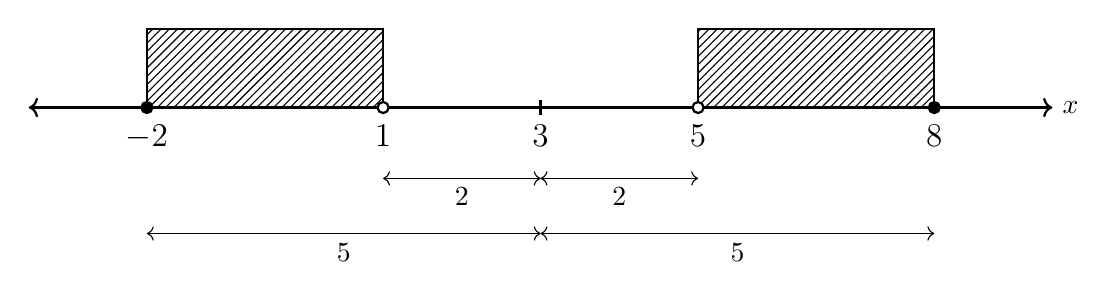
\begin{tikzpicture}
    \draw[thick,<->] (-6.5,0) -- (6.5,0) node[right] {$x$};
    \fill[pattern=north east lines] (-5,0) rectangle (-2,1);
    \fill[pattern=north east lines] (2,0) rectangle (5,1);
    \draw[thick] (-5,0) -- (-5,1) -- (-2,1) -- (-2,0);
    \draw[thick] (2,0) -- (2,1) -- (5,1) -- (5,0);
    \draw (-5,-0.1) node[below] {\large{$-2$}};
    \draw (-2,-0.1) node[below] {\large{$1$}};
    \draw (0,-0.1) node[below] {\large{$3$}};
    \draw (2,-0.1) node[below] {\large{$5$}};
    \draw (5,-0.1) node[below] {\large{$8$}};
    \draw[thick] (0,-0.1) -- (0,0.1);
    \draw[<->] (0,-0.9) -- (-2,-0.9) node[midway, below] {$2$};
    \draw[<->] (0,-0.9) -- (2,-0.9) node[midway, below] {$2$};
    \draw[<->] (0,-1.6) -- (-5,-1.6) node[midway, below] {$5$};
    \draw[<->] (0,-1.6) -- (5,-1.6) node[midway, below] {$5$};
    \draw[fill=black, thick] (-5,0) circle (2pt);
    \draw[fill=white, thick] (-2,0) circle (2pt);
    \draw[fill=white, thick] (2,0) circle (2pt);
    \draw[fill=black, thick] (5,0) circle (2pt);
                    \end{tikzpicture}
                \end{center}
                Jadi solusi dari ketaksamaan tersebut adalah $-2\leq x<1$ atau $5<x\leq 8$. Dalam notasi interval, solusi tersebut dapat ditulis sebagai $\colorlet{oldcolor}{.}
        \color{red}
        \setlength{\fboxrule}{1pt} \boxed{\color{oldcolor}[-2, 1) \cup (5, 8]}\color{oldcolor}$.
            }
            \end{jawab}
            \item Diketahui garis $\ell_1$ dengan gradien $m_1=\frac{2}{3}$ dan garis $\ell_2$ berpotongan tegak lurus dengan $\ell_1$ di titik $(4,-1)$. Dapatkan persamaan garis $\ell_2$. \\
            Gambarkan kedua garis $\ell_1$ dan $\ell_2$ pada satu bidang koordinat.
            \begin{jawab}[gradien garis, garis tegak lurus, persamaan garis]{~\\
                Ingat kembali bahwa dua garis dengan gradien $m_1$ dan $m_2$ saling tegak lurus jika $\colorlet{oldcolor}{.}
        \color{blue}
        \setlength{\fboxrule}{1pt} \boxed{\color{oldcolor}m_1\cdot m_2=-1}\color{oldcolor}$. Karena $m_1=\frac{2}{3}$, diperoleh
                \begin{align*}
                    \frac{2}{3}\cdot m_2 = -1 \implies \colorlet{oldcolor}{.}
        \color{blue}
        \setlength{\fboxrule}{1pt} \boxed{\color{oldcolor}m_2 = -\frac{3}{2}}\color{oldcolor}.
                \end{align*}
                Garis $\ell_2$ melalui titik $(4,-1)$ dengan gradien $-\frac{3}{2}$, sehingga dengan rumus $y - y_1 = m(x - x_1)$ diperoleh
                \begin{align*}
                    y - (-1) &= -\frac{3}{2}(x - 4)\\
                    y + 1 &= -\frac{3}{2}x + 6\\
                    y &= -\frac{3}{2}x + 5.
                \end{align*}
                Jadi persamaan garis $\ell_2$ adalah $\colorlet{oldcolor}{.}
        \color{red}
        \setlength{\fboxrule}{1pt} \boxed{\color{oldcolor}y = -\frac{3}{2}x + 5}\color{oldcolor}$ atau $3x+2y=10$.\\
                Selanjutnya, karena $\ell_1$ juga melalui titik potong $(4,-1)$ dengan gradien $\frac{2}{3}$, persamaan garis $\ell_1$ adalah
                \begin{align*}
                    y + 1 = \frac{2}{3}(x - 4) \implies y = \frac{2}{3}x - \frac{11}{3}.
                \end{align*}
                Sebagai bantuan menggambar, garis $\ell_1$ melalui titik $(1,-3)$ dan $(4,-1)$, sedangkan garis $\ell_2$ melalui titik $(0,5)$ dan $(4,-1)$. Sketsa kedua garis tersebut adalah sebagai berikut
                \begin{center}
                    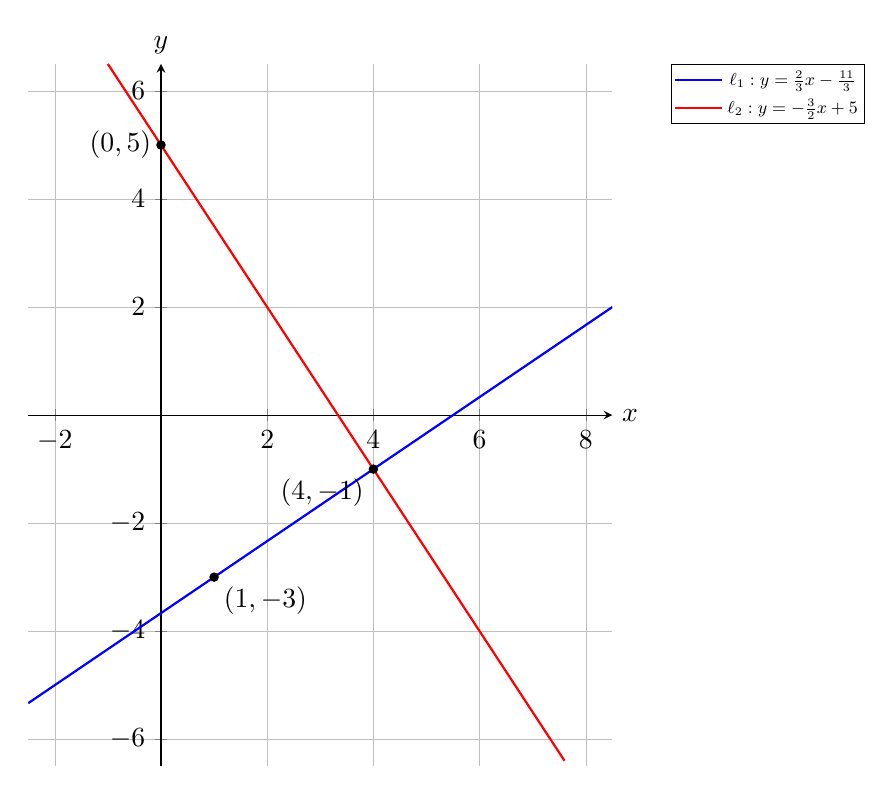
\begin{tikzpicture}
                        \begin{axis}[
        axis lines = middle,
        xlabel = $x$,
        ylabel = {$y$},
        xtick={-2,0,...,8},
        ytick={-6,-4,...,6},
        xmin=-2.5, xmax=8.5,
        ymin=-6.5, ymax=6.5,
        width=9cm,
        height=10.5cm,
        grid=both,
        grid style={line width=.1pt, draw=gray!10},
        major grid style={line width=.2pt,draw=gray!50},
        x label style={anchor=west}, % label x ke kanan
        y label style={anchor=south}, % label y ke atas
        samples=200,
        legend style={
                at={(1.1,1)},
                anchor=north west,
                font=\small,         % mengecilkan ukuran font
                row sep=1pt,         % jarak antar baris legend
                inner sep=1pt,       % margin dalam kotak legend
                nodes={scale=0.7}    % skalakan isi legend
            }
    ]
\addplot[domain=-2.5:8.5, color=blue, thick, samples=2] {2*x/3-11/3};
\addlegendentry{$\ell_1: y=\frac{2}{3}x-\frac{11}{3}$}
\addplot[domain=-1:7.6, color=red, thick, samples=2] {-3*x/2+5};
\addlegendentry{$\ell_2: y=-\frac{3}{2}x+5$}
\draw[fill=black] (4,-1) circle (1.5pt) node[below left] {$(4,-1)$};
\draw[fill=black] (1,-3) circle (1.5pt) node[below right] {$(1,-3)$};
\draw[fill=black] (0,5) circle (1.5pt) node[left] {$(0,5)$};
\end{axis}
                    \end{tikzpicture}
                \end{center}
            }
            \end{jawab}
            \item Diketahui $f(x)=x^2-4x$.
            \begin{enumerate}
                \item Tentukan domain alami untuk $x$ agar $f(x)$ mempunyai invers.
                \item Dapatkan $f^{-1}(x)$, domain, dan rangenya.
            \end{enumerate}
            \begin{jawab}[fungsi satu-satu, melengkapkan kuadrat, fungsi invers]{
                \begin{enumerate}
                    \item Suatu fungsi mempunyai invers jika fungsi tersebut satu-satu (injektif). Dengan melengkapkan kuadrat, diperoleh
                    \begin{align*}
                        f(x) = x^2 - 4x = (x^2-4x+4)-4 = \colorlet{oldcolor}{.}
        \color{blue}
        \setlength{\fboxrule}{1pt} \boxed{\color{oldcolor}(x-2)^2 - 4}\color{oldcolor}.
                    \end{align*}
                    Grafik $f$ merupakan parabola terbuka ke atas dengan titik puncak $(2,-4)$. Pada seluruh $\mathbb{R}$, fungsi $f$ tidak satu-satu, misalnya $f(0)=f(4)=0$. Agar satu-satu, domain $f$ harus dibatasi pada salah satu sisi titik puncak, yaitu $x\geq 2$ (atau $x\leq 2$). Dalam pembahasan ini dipilih
                    \begin{align*}
                        \colorlet{oldcolor}{.}
        \color{red}
        \setlength{\fboxrule}{1pt} \boxed{\color{oldcolor}D(f) = [2,\infty)}\color{oldcolor}.
                    \end{align*}
                    \item Misalkan $y=f(x)$ dengan $x\geq 2$, kemudian selesaikan sehingga terbentuk $x$ dalam fungsi $y$. Diperoleh
                    \begin{align*}
                        y &= (x-2)^2 - 4\\
                        (x-2)^2 &= y + 4\\
                        x - 2 &= \sqrt{y+4} \quad (\text{karena } x-2\geq 0)\\
                        x &= 2 + \sqrt{y+4}.
                    \end{align*}
                    Dari sini didapatkan $x = f^{-1}(y) = 2+\sqrt{y+4}$. Dengan mengganti $y$ dengan $x$, diperoleh $\colorlet{oldcolor}{.}
        \color{red}
        \setlength{\fboxrule}{1pt} \boxed{\color{oldcolor}f^{-1}(x) = 2 + \sqrt{x+4}}\color{oldcolor}$.\\
                    Selanjutnya, karena $x\geq 2$, nilai $(x-2)^2-4\geq -4$, sehingga range dari $f$ adalah $R(f)=[-4,\infty)$. Domain dari fungsi invers adalah range dari fungsi asli dan range dari fungsi invers adalah domain dari fungsi asli, yaitu
                    \begin{align*}
                        \colorlet{oldcolor}{.}
        \color{red}
        \setlength{\fboxrule}{1pt} \boxed{\color{oldcolor}D(f^{-1}) = R(f) = [-4, \infty)}\color{oldcolor} \quad\text{dan}\quad \colorlet{oldcolor}{.}
        \color{red}
        \setlength{\fboxrule}{1pt} \boxed{\color{oldcolor}R(f^{-1}) = D(f) = [2, \infty)}\color{oldcolor}.
                    \end{align*}
                    \textit{Catatan:} jika pada (a) dipilih domain $(-\infty,2]$, maka diperoleh $f^{-1}(x) = 2 - \sqrt{x+4}$ dengan domain $[-4,\infty)$ dan range $(-\infty,2]$.
                \end{enumerate}
            }
            \end{jawab}
            \item Diberikan fungsi
            \begin{align*}
                f(x)=\begin{cases}
                    \frac{x^2-9}{x+3}, &x\neq -3\\
                    k, &x=-3
                \end{cases}
            \end{align*}
            \begin{enumerate}
                \item Tentukan nilai $k$ agar $f(-3)=\displaystyle\lim_{x\to -3} f(x)$.
                \item Dengan memberi $k$ pada $\displaystyle\lim_{x\to-3} f(x)$, tunjukkan bahwa $f(x)$ dapat dinyatakan sebagai fungsi polinomial.
            \end{enumerate}
            \begin{jawab}[limit fungsi, fungsi kontinu, polinomial]{
                \begin{enumerate}
                    \item Diperhatikan bahwa untuk \(x = -3\), \(\colorlet{oldcolor}{.}
        \color{blue}
        \setlength{\fboxrule}{1pt} \boxed{\color{oldcolor}f(-3) = k}\color{oldcolor}\). Karena limit di $x=-3$ artinya nilai fungsi di sekitar $x=-3$ tetapi $x\neq -3$, didapatkan limitnya adalah
                    \begin{align*}
                        \lim_{x \to -3} f(x) = \lim_{x \to -3} \frac{x^2 - 9}{x + 3} = \lim_{x \to -3} \frac{(x-3)(x+3)}{x+3} = \lim_{x \to -3} (x-3) = -3-3 = \colorlet{oldcolor}{.}
        \color{blue}
        \setlength{\fboxrule}{1pt} \boxed{\color{oldcolor}-6}\color{oldcolor}.
                    \end{align*}
                    Karena haruslah $\displaystyle f(-3)=\lim_{x\to -3} f(x)$, diperoleh $\colorlet{oldcolor}{.}
        \color{red}
        \setlength{\fboxrule}{1pt} \boxed{\color{oldcolor}k=-6}\color{oldcolor}$.
                    \item Diperhatikan bahwa untuk $x\neq -3$, berlaku
                    \begin{align*}
                        f(x) = \frac{x^2 - 9}{x + 3} = \frac{(x-3)(x+3)}{x+3} = x - 3.
                    \end{align*}
                    Untuk $x=-3$, dengan $k=-6$ berlaku $f(-3)=-6=(-3)-3$, yang juga sama dengan nilai $x-3$ saat $x=-3$. Dengan demikian, untuk setiap $x\in\mathbb{R}$ berlaku $f(x)=x-3$, sehingga $f(x)$ dapat dinyatakan sebagai polinomial
                    \begin{align*}
                        \colorlet{oldcolor}{.}
        \color{red}
        \setlength{\fboxrule}{1pt} \boxed{\color{oldcolor}f(x) = x - 3}\color{oldcolor}.
                    \end{align*}
                \end{enumerate}
            }
            \end{jawab}
            \item Diketahui $f(x)=(\sqrt{x}+2x^2+1)^5$.\\
            Dengan aturan rantai, dapatkan turunan pertama dari $f(x)$.
            \begin{jawab}[turunan fungsi, aturan rantai]{~\\
                Ingat kembali aturan rantai untuk turunan fungsi, yaitu
                \[
                \colorlet{oldcolor}{.}
        \color{blue}
        \setlength{\fboxrule}{1pt} \boxed{\color{oldcolor}\frac{d}{dx}[h(g(x))] = h'(g(x)) \cdot g'(x)}\color{oldcolor}.
                \]
                Dapat dimisalkan $\colorlet{oldcolor}{.}
        \color{blue}
        \setlength{\fboxrule}{1pt} \boxed{\color{oldcolor}u=g(x) = \sqrt{x}+2x^2+1}\color{oldcolor}$ sehingga $\colorlet{oldcolor}{.}
        \color{blue}
        \setlength{\fboxrule}{1pt} \boxed{\color{oldcolor}h(u) = u^{5}}\color{oldcolor}$, dan diperoleh
                \begin{align*}
                    \colorlet{oldcolor}{.}
        \color{blue}
        \setlength{\fboxrule}{1pt} \boxed{\color{oldcolor}h'(u) = 5u^{4}}\color{oldcolor} \quad \text{dan}\quad
                    \colorlet{oldcolor}{.}
        \color{blue}
        \setlength{\fboxrule}{1pt} \boxed{\color{oldcolor}g'(x) = \frac{1}{2\sqrt{x}}+4x}\color{oldcolor}.
                \end{align*}
                Dengan demikian, diperoleh
                \begin{align*}
                    f'(x) &= h'(u) \cdot g'(x)\\
                    &= 5u^{4} \cdot \left(\frac{1}{2\sqrt{x}}+4x\right)\\
                    &= \colorlet{oldcolor}{.}
        \color{red}
        \setlength{\fboxrule}{1pt} \boxed{\color{oldcolor}5\left(\sqrt{x}+2x^2+1\right)^{4} \left(\frac{1}{2\sqrt{x}}+4x\right)}\color{oldcolor}.
                \end{align*}
            }
            \end{jawab}
        \end{enumerate}
               \newpage
 \begin{center}
	{\underline{\textbf{\MakeUppercase{Soal dan Pembahasan ETS Kalkulus 1 Tahun 2025/2026}}}}
    \end{center}

    \begin{center}
	\begin{tabular}{lcl}
		Mata kuliah/SKS & : & Kalkulus 1 ( SM234101 ) / 3 SKS\\
		Hari, Tanggal & : & Selasa, 14 Oktober 2025\\
		Waktu & : & 15.30 - 17.10 / 100 menit\\
		Sifat & : & Tertutup\\
		Kelas & : & 30-39\\
  ~
	\end{tabular}

    \noindent\rule{\textwidth}{2.pt}
        \end{center}
        \begin{enumerate}
            \item Dapatkan penyelesaian dari pertidaksamaan
            \begin{align*}
                2\leq x^2-2\leq 7.
            \end{align*}
            \begin{jawab}[pertidaksamaan kuadrat, pertidaksamaan ganda, notasi interval]{~\\
                Dengan menambahkan $2$ pada ketiga ruas, didapatkan
                \begin{align*}
                    4\leq x^2\leq 9.
                \end{align*}
                Pertidaksamaan ganda tersebut dapat dipecah menjadi dua bagian:
                \begin{itemize}
                    \item $x^2\geq 4$, yaitu $x^2-4=(x-2)(x+2)\geq 0$. Dengan uji titik, diperoleh $\colorlet{oldcolor}{.}
        \color{blue}
        \setlength{\fboxrule}{1pt} \boxed{\color{oldcolor}x\leq -2 \quad\vee\quad x\geq 2}\color{oldcolor}$.
                    \item $x^2\leq 9$, yaitu $x^2-9=(x-3)(x+3)\leq 0$. Dengan uji titik, diperoleh $\colorlet{oldcolor}{.}
        \color{blue}
        \setlength{\fboxrule}{1pt} \boxed{\color{oldcolor}-3\leq x\leq 3}\color{oldcolor}$.
                \end{itemize}
                Penyelesaian dari pertidaksamaan adalah irisan dari kedua bagian tersebut, yang dapat digambarkan pada garis bilangan sebagai berikut
                \begin{center}
                    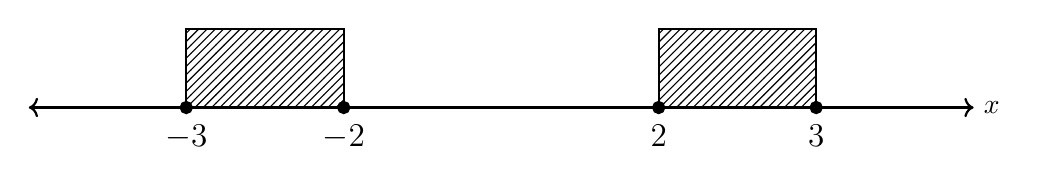
\begin{tikzpicture}
    \draw[thick,<->] (-6,0) -- (6,0) node[right] {$x$};
    \fill[pattern=north east lines] (-4,0) rectangle (-2,1);
    \fill[pattern=north east lines] (2,0) rectangle (4,1);
    \draw[thick] (-4,0) -- (-4,1) -- (-2,1) -- (-2,0);
    \draw[thick] (2,0) -- (2,1) -- (4,1) -- (4,0);
    \draw (-4,-0.1) node[below] {\large{$-3$}};
    \draw (-2,-0.1) node[below] {\large{$-2$}};
    \draw (2,-0.1) node[below] {\large{$2$}};
    \draw (4,-0.1) node[below] {\large{$3$}};
    \draw[fill=black, thick] (-4,0) circle (2pt);
    \draw[fill=black, thick] (-2,0) circle (2pt);
    \draw[fill=black, thick] (2,0) circle (2pt);
    \draw[fill=black, thick] (4,0) circle (2pt);
                    \end{tikzpicture}
                \end{center}
                Jadi penyelesaian dari pertidaksamaan tersebut adalah $-3\leq x\leq -2$ atau $2\leq x\leq 3$. Dalam notasi interval, dapat ditulis sebagai $\colorlet{oldcolor}{.}
        \color{red}
        \setlength{\fboxrule}{1pt} \boxed{\color{oldcolor}[-3, -2] \cup [2, 3]}\color{oldcolor}$.
            }
            \end{jawab}
            \item Gunakan grafik dasar $x=y^2$ dan sifat pergeseran/translasi untuk menggambar parabola $x=y^2+2y+3$.
            \begin{jawab}[parabola, melengkapkan kuadrat, translasi grafik]{~\\
                Kurva dasar $x=y^2$ merupakan parabola yang terbuka ke kanan dengan titik puncak $(0,0)$. Selanjutnya, bentuk $x = y^2 + 2y + 3$ diubah dengan cara melengkapkan kuadrat, yaitu
                \begin{align*}
                    x &= y^2 + 2y + 3\\
                    &= (y^2 + 2y + 1) - 1 + 3\\
                    &= \colorlet{oldcolor}{.}
        \color{blue}
        \setlength{\fboxrule}{1pt} \boxed{\color{oldcolor}(y+1)^2 + 2}\color{oldcolor}.
                \end{align*}
                Ingat kembali bahwa mengganti $y$ dengan $y+1$ berarti menggeser grafik sejauh $1$ satuan ke bawah, dan menambahkan konstanta $2$ pada $x$ berarti menggeser grafik sejauh $2$ satuan ke kanan. Dengan demikian, proses translasinya adalah sebagai berikut.
                \begin{enumerate}
                    \item[(i)] Gambar kurva dasar $x=y^2$ dengan titik puncak $(0,0)$.
                    \item[(ii)] Geser kurva $x=y^2$ sejauh $1$ satuan ke bawah, sehingga diperoleh kurva $x=(y+1)^2$ dengan titik puncak $(0,-1)$.
                    \item[(iii)] Geser kurva $x=(y+1)^2$ sejauh $2$ satuan ke kanan, sehingga diperoleh kurva $x=(y+1)^2+2$ dengan titik puncak $\colorlet{oldcolor}{.}
        \color{blue}
        \setlength{\fboxrule}{1pt} \boxed{\color{oldcolor}(2,-1)}\color{oldcolor}$.
                \end{enumerate}
                Sebagai bantuan, titik potong kurva dengan sumbu-$x$ ($y=0$) adalah $x=3$, yaitu titik $(3,0)$, sedangkan kurva tidak memotong sumbu-$y$ karena $x=(y+1)^2+2\geq 2$. Sketsa grafiknya adalah sebagai berikut.
                \begin{center}
                    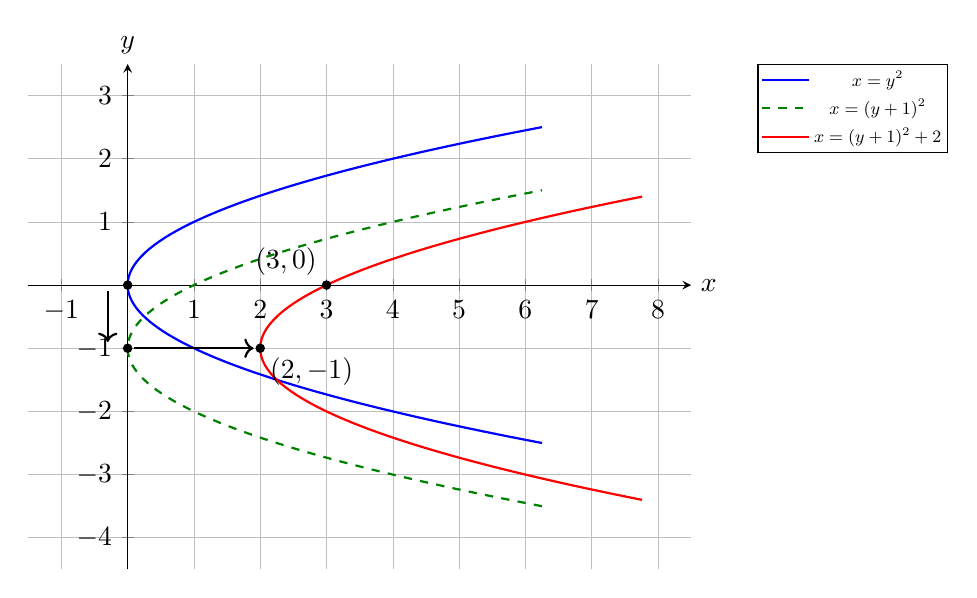
\begin{tikzpicture}
                        \begin{axis}[
        axis lines = middle,
        xlabel = $x$,
        ylabel = {$y$},
        xtick={-1,0,...,8},
        ytick={-4,-3,...,3},
        xmin=-1.5, xmax=8.5,
        ymin=-4.5, ymax=3.5,
        width=10cm,
        height=8cm,
        grid=both,
        grid style={line width=.1pt, draw=gray!10},
        major grid style={line width=.2pt,draw=gray!50},
        x label style={anchor=west}, % label x ke kanan
        y label style={anchor=south}, % label y ke atas
        samples=200,
        legend style={
                at={(1.1,1)},
                anchor=north west,
                font=\small,         % mengecilkan ukuran font
                row sep=1pt,         % jarak antar baris legend
                inner sep=1pt,       % margin dalam kotak legend
                nodes={scale=0.7}    % skalakan isi legend
            }
    ]
\addplot[domain=-2.5:2.5, color=blue, thick] ({(x)*(x)},{x});
\addlegendentry{$x=y^2$}
\addplot[domain=-3.5:1.5, color=green!50!black, thick, dashed] ({(x+1)*(x+1)},{x});
\addlegendentry{$x=(y+1)^2$}
\addplot[domain=-3.4:1.4, color=red, thick] ({(x+1)*(x+1)+2},{x});
\addlegendentry{$x=(y+1)^2+2$}
\draw[fill=black] (0,0) circle (1.5pt);
\draw[fill=black] (0,-1) circle (1.5pt);
\draw[fill=black] (2,-1) circle (1.5pt) node[below right] {$(2,-1)$};
\draw[fill=black] (3,0) circle (1.5pt) node[above left] {$(3,0)$};
\draw[->, thick] (-0.3,-0.1) -- (-0.3,-0.9);
\draw[->, thick] (0.1,-1) -- (1.9,-1);
\end{axis}
                    \end{tikzpicture}
                \end{center}
                Jadi parabola $x = y^2 + 2y + 3$ adalah
                \[\colorlet{oldcolor}{.}
        \color{red}
        \setlength{\fboxrule}{1pt} \boxed{\color{oldcolor}\text{parabola } x=y^2 \text{ yang digeser 1 satuan ke bawah dan 2 satuan ke kanan}}\color{oldcolor}.\]
            }
            \end{jawab}
            \item Tentukan domain dari fungsi $(f\circ g)(x)$ jika diketahui fungsi $g(x)=2x+3$ dengan $0\leq x<3$ dan fungsi $f$ terdefinisi pada interval $-1\leq x <5$.
            \begin{jawab}[fungsi komposisi, domain fungsi komposisi]{~\\
                Diketahui $\colorlet{oldcolor}{.}
        \color{blue}
        \setlength{\fboxrule}{1pt} \boxed{\color{oldcolor}D(g)=[0,3)}\color{oldcolor}$ dan $\colorlet{oldcolor}{.}
        \color{blue}
        \setlength{\fboxrule}{1pt} \boxed{\color{oldcolor}D(f)=[-1,5)}\color{oldcolor}$. Domain dari fungsi komposisi $f\circ g$ adalah semua nilai $x$ pada domain $g$ sehingga nilai dari $g(x)$ berada pada domain $f$, yang dapat dirumuskan sebagai
                \begin{align*}
                    \colorlet{oldcolor}{.}
        \color{blue}
        \setlength{\fboxrule}{1pt} \boxed{\color{oldcolor}D(f\circ g) = \{x \in D(g) : g(x) \in D(f)\} = \{x \in [0, 3) : -1\leq 2x+3 < 5\}}\color{oldcolor}.
                \end{align*}
                Selanjutnya, diselesaikan pertidaksamaan
                \begin{align*}
                    -1 &\leq 2x+3 < 5\\
                    -4 &\leq 2x < 2\\
                    -2 &\leq x < 1.
                \end{align*}
                Dengan mengiriskan dengan $D(g)=[0,3)$, didapatkan
                \begin{align*}
                    D(f\circ g) = [0,3)\cap[-2,1) = \colorlet{oldcolor}{.}
        \color{red}
        \setlength{\fboxrule}{1pt} \boxed{\color{oldcolor}[0,1)}\color{oldcolor}.
                \end{align*}
            }
            \end{jawab}
            \item Diberikan fungsi $f(x)=\left|\dfrac{x^2-9}{x-3}\right|$. Dapatkan titik $x$ di mana membuat fungsi $f(x)$ diskontinu?\\
            Dapatkan nilai fungsi $f(x)$ pada titik tersebut agar menjadi kontinu dan sketsa grafik fungsi tersebut.
            \begin{jawab}[fungsi kontinu, limit, nilai mutlak, sketsa grafik]{~\\
                Diperhatikan bahwa penyebut $x-3$ bernilai nol saat $x=3$, sehingga $f(3)$ tidak terdefinisi. Karena syarat pertama kekontinuan (yaitu $f(a)$ terdefinisi) tidak terpenuhi, maka fungsi $f$ $\colorlet{oldcolor}{.}
        \color{red}
        \setlength{\fboxrule}{1pt} \boxed{\color{oldcolor}\text{diskontinu di } x=3}\color{oldcolor}$. Untuk $x\neq 3$, fungsi dapat disederhanakan menjadi
                \begin{align*}
                    f(x) = \left|\frac{(x-3)(x+3)}{x-3}\right| = \colorlet{oldcolor}{.}
        \color{blue}
        \setlength{\fboxrule}{1pt} \boxed{\color{oldcolor}|x+3|}\color{oldcolor}, \quad x\neq 3.
                \end{align*}
                Selanjutnya, limit di $x=3$ adalah
                \begin{align*}
                    \lim_{x\to 3} f(x) = \lim_{x\to 3} |x+3| = |3+3| = 6.
                \end{align*}
                Karena limitnya ada, diskontinuitas di $x=3$ dapat dihapus (\textit{removable}). Agar $f$ kontinu di $x=3$, haruslah $\displaystyle f(3)=\lim_{x\to 3} f(x)$, sehingga didefinisikan $\colorlet{oldcolor}{.}
        \color{red}
        \setlength{\fboxrule}{1pt} \boxed{\color{oldcolor}f(3)=6}\color{oldcolor}$.\\
                Dengan definisi tersebut, $f(x)=|x+3|$ untuk semua $x\in\mathbb{R}$, yaitu
                \begin{align*}
                    f(x) = |x+3| = \begin{cases}
                        x+3, & x\geq -3\\
                        -(x+3), & x<-3
                    \end{cases}
                \end{align*}
                yang grafiknya berbentuk huruf ``V'' dengan titik puncak $(-3,0)$. Sketsa grafiknya adalah sebagai berikut, dengan titik $(3,6)$ yang semula berlubang kini terisi.
                \begin{center}
                    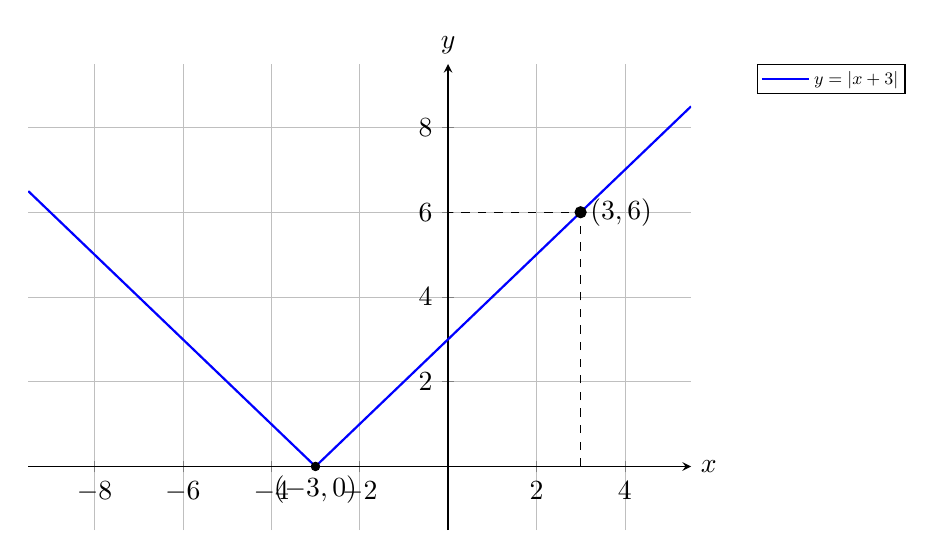
\begin{tikzpicture}
                        \begin{axis}[
        axis lines = middle,
        xlabel = $x$,
        ylabel = {$y$},
        xtick={-8,-6,...,4},
        ytick={0,2,...,8},
        xmin=-9.5, xmax=5.5,
        ymin=-1.5, ymax=9.5,
        width=10cm,
        height=7.5cm,
        grid=both,
        grid style={line width=.1pt, draw=gray!10},
        major grid style={line width=.2pt,draw=gray!50},
        x label style={anchor=west}, % label x ke kanan
        y label style={anchor=south}, % label y ke atas
        samples=200,
        legend style={
                at={(1.1,1)},
                anchor=north west,
                font=\small,         % mengecilkan ukuran font
                row sep=1pt,         % jarak antar baris legend
                inner sep=1pt,       % margin dalam kotak legend
                nodes={scale=0.7}    % skalakan isi legend
            }
    ]
\addplot[domain=-9.5:5.5, color=blue, thick] {abs(x+3)};
\addlegendentry{$y=|x+3|$}
\draw[fill=black] (-3,0) circle (1.5pt) node[below] {$(-3,0)$};
\draw[fill=black] (3,6) circle (2pt) node[right] {$(3,6)$};
\draw[dashed] (3,0) -- (3,6) -- (0,6);
\end{axis}
                    \end{tikzpicture}
                \end{center}
            }
            \end{jawab}
            \item Dengan diferensiasi implisit, dapatkan $\frac{dy}{dx}$ dari $x^3y^2-3xy^2+x=1$.
            \begin{jawab}[diferensiasi implisit, aturan perkalian, aturan rantai]{~\\
                Kita turunkan kedua ruas terhadap $x$, dengan mengingat bahwa $y$ adalah fungsi dari $x$:
                \begin{align*}
                    \frac{d}{dx}(x^3y^2) - \frac{d}{dx}(3xy^2) + \frac{d}{dx}(x) = \frac{d}{dx}(1).
                \end{align*}
                Dengan aturan perkalian dan aturan rantai (ingat $\frac{d}{dx}(y^2)=2y\frac{dy}{dx}$), diperoleh
                \begin{align*}
                    \colorlet{oldcolor}{.}
        \color{blue}
        \setlength{\fboxrule}{1pt} \boxed{\color{oldcolor}\frac{d}{dx}(x^3y^2) = 3x^2y^2 + 2x^3y\frac{dy}{dx}}\color{oldcolor} \quad\text{dan}\quad \colorlet{oldcolor}{.}
        \color{blue}
        \setlength{\fboxrule}{1pt} \boxed{\color{oldcolor}\frac{d}{dx}(3xy^2) = 3y^2 + 6xy\frac{dy}{dx}}\color{oldcolor}.
                \end{align*}
                Dengan demikian, diperoleh
                \begin{align*}
                    3x^2y^2 + 2x^3y\frac{dy}{dx} - 3y^2 - 6xy\frac{dy}{dx} + 1 &= 0\\
                    (2x^3y - 6xy)\frac{dy}{dx} &= 3y^2 - 3x^2y^2 - 1\\
                    \frac{dy}{dx} &= \colorlet{oldcolor}{.}
        \color{red}
        \setlength{\fboxrule}{1pt} \boxed{\color{oldcolor}\frac{3y^2 - 3x^2y^2 - 1}{2x^3y - 6xy}}\color{oldcolor},
                \end{align*}
                atau dapat juga ditulis $\displaystyle\frac{dy}{dx} = \frac{3y^2(1-x^2) - 1}{2xy(x^2-3)}$.
            }
            \end{jawab}
        \end{enumerate}
 \newpage
 \begin{center}
	{\underline{\textbf{\MakeUppercase{Soal dan Pembahasan ETS Matematika Tahun 2025/2026}}}}
    \end{center}

    \begin{center}
	\begin{tabular}{lcl}
		Mata kuliah/SKS & : & Matematika ( SM234152 ) / 2 SKS\\
		Hari, Tanggal & : & Jumat, 17 Oktober 2025\\
		Waktu & : & 07.00 - 08.40 / 100 menit\\
		Sifat & : & Tertutup\\
		Kelas & : & 1-8\\
  ~
	\end{tabular}

    \noindent\rule{\textwidth}{2.pt}
        \end{center}
\begin{enumerate}
    \item Diberikan SPL
    \begin{align*}
        x+y+2z &= 8\\
        -x-2y+3z &= 1\\
        3x-7y+4z &= 10
    \end{align*}
    \begin{enumerate}
        \item Nyatakan SPL tersebut dalam bentuk persamaan matriks $A\mathbf{x}=b$.
        \item Menggunakan Eliminasi Gauss, carilah solusi (jika ada) dari SPL tersebut.
    \end{enumerate}
    \begin{jawab}[sistem persamaan linear, matriks, eliminasi Gauss]{
        \begin{enumerate}
            \item Koefisien dari variabel $x,y,z$ pada setiap persamaan disusun menjadi matriks $A$, variabelnya menjadi vektor $\mathbf{x}$, dan ruas kanan menjadi vektor $b$. Diperoleh
            \begin{align*}
                \colorlet{oldcolor}{.}
        \color{red}
        \setlength{\fboxrule}{1pt} \boxed{\color{oldcolor}\underbrace{\begin{bmatrix}
                    1 & 1 & 2\\
                    -1 & -2 & 3\\
                    3 & -7 & 4
                \end{bmatrix}}_{A}
                \underbrace{\begin{bmatrix}
                    x\\ y\\ z
                \end{bmatrix}}_{\mathbf{x}}
                =
                \underbrace{\begin{bmatrix}
                    8\\ 1\\ 10
                \end{bmatrix}}_{b}}\color{oldcolor}.
            \end{align*}
            \item Dibentuk matriks lengkap (\textit{augmented matrix}) $[A\,|\,b]$, kemudian dilakukan operasi baris elementer (OBE) sampai terbentuk matriks eselon baris.
            \begin{align*}
                \left[\begin{array}{ccc|c}
                    1 & 1 & 2 & 8\\
                    -1 & -2 & 3 & 1\\
                    3 & -7 & 4 & 10
                \end{array}\right]
                \xrightarrow[R_3 - 3R_1]{R_2 + R_1}
                \left[\begin{array}{ccc|c}
                    1 & 1 & 2 & 8\\
                    0 & -1 & 5 & 9\\
                    0 & -10 & -2 & -14
                \end{array}\right]
                \xrightarrow{R_3 - 10R_2}
                \left[\begin{array}{ccc|c}
                    1 & 1 & 2 & 8\\
                    0 & -1 & 5 & 9\\
                    0 & 0 & -52 & -104
                \end{array}\right]
            \end{align*}
            Matriks terakhir sudah berbentuk eselon baris dan setiap kolom variabel memiliki pivot, sehingga SPL memiliki solusi tunggal. Selanjutnya, dilakukan substitusi balik:
            \begin{align*}
                -52z &= -104 \implies \colorlet{oldcolor}{.}
        \color{blue}
        \setlength{\fboxrule}{1pt} \boxed{\color{oldcolor}z = 2}\color{oldcolor}\\
                -y + 5z &= 9 \implies -y + 10 = 9 \implies \colorlet{oldcolor}{.}
        \color{blue}
        \setlength{\fboxrule}{1pt} \boxed{\color{oldcolor}y = 1}\color{oldcolor}\\
                x + y + 2z &= 8 \implies x + 1 + 4 = 8 \implies \colorlet{oldcolor}{.}
        \color{blue}
        \setlength{\fboxrule}{1pt} \boxed{\color{oldcolor}x = 3}\color{oldcolor}
            \end{align*}
            Sebagai pengecekan, $-3-2(1)+3(2)=1$ dan $3(3)-7(1)+4(2)=10$, sesuai dengan SPL. Jadi solusi dari SPL tersebut adalah $\colorlet{oldcolor}{.}
        \color{red}
        \setlength{\fboxrule}{1pt} \boxed{\color{oldcolor}(x,y,z)=(3,1,2)}\color{oldcolor}$.
        \end{enumerate}
    }
    \end{jawab}
    \item Carilah himpunan penyelesaian dari pertidaksamaan
    \begin{align*}
        1<|3x-4|\leq 6.
    \end{align*}
    \begin{jawab}[pertidaksamaan nilai mutlak, notasi interval]{~\\
        Pertidaksamaan ganda tersebut dapat dipecah menjadi dua bagian. Ingat kembali sifat nilai mutlak, yaitu untuk $a>0$ berlaku
        \begin{align*}
            \colorlet{oldcolor}{.}
        \color{blue}
        \setlength{\fboxrule}{1pt} \boxed{\color{oldcolor}|u|\leq a \iff -a\leq u\leq a}\color{oldcolor} \quad\text{dan}\quad \colorlet{oldcolor}{.}
        \color{blue}
        \setlength{\fboxrule}{1pt} \boxed{\color{oldcolor}|u|> a \iff u<-a \;\vee\; u>a}\color{oldcolor}.
        \end{align*}
        \begin{itemize}
            \item Untuk $|3x-4|\leq 6$, diperoleh
            \begin{align*}
                -6\leq 3x-4\leq 6 \implies -2\leq 3x\leq 10 \implies -\frac{2}{3}\leq x\leq \frac{10}{3}.
            \end{align*}
            \item Untuk $|3x-4|> 1$, diperoleh
            \begin{align*}
                3x-4<-1 \quad\vee\quad 3x-4>1 \implies x<1 \quad\vee\quad x>\frac{5}{3}.
            \end{align*}
        \end{itemize}
        Himpunan penyelesaian adalah irisan dari kedua bagian tersebut, yang dapat digambarkan pada garis bilangan sebagai berikut
        \begin{center}
            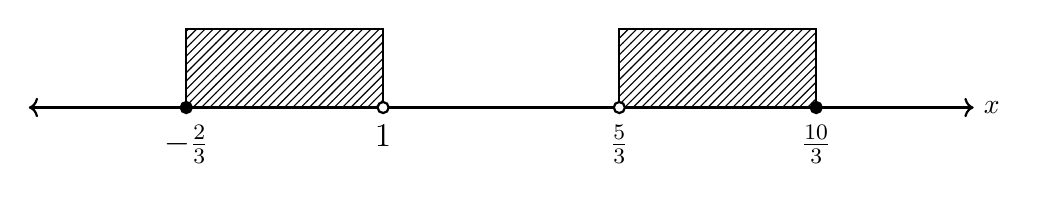
\begin{tikzpicture}
    \draw[thick,<->] (-6,0) -- (6,0) node[right] {$x$};
    \fill[pattern=north east lines] (-4,0) rectangle (-1.5,1);
    \fill[pattern=north east lines] (1.5,0) rectangle (4,1);
    \draw[thick] (-4,0) -- (-4,1) -- (-1.5,1) -- (-1.5,0);
    \draw[thick] (1.5,0) -- (1.5,1) -- (4,1) -- (4,0);
    \draw (-4,-0.1) node[below] {\large{$-\frac{2}{3}$}};
    \draw (-1.5,-0.1) node[below] {\large{$1$}};
    \draw (1.5,-0.1) node[below] {\large{$\frac{5}{3}$}};
    \draw (4,-0.1) node[below] {\large{$\frac{10}{3}$}};
    \draw[fill=black, thick] (-4,0) circle (2pt);
    \draw[fill=white, thick] (-1.5,0) circle (2pt);
    \draw[fill=white, thick] (1.5,0) circle (2pt);
    \draw[fill=black, thick] (4,0) circle (2pt);
            \end{tikzpicture}
        \end{center}
        Jadi himpunan penyelesaiannya adalah $\colorlet{oldcolor}{.}
        \color{red}
        \setlength{\fboxrule}{1pt} \boxed{\color{oldcolor}\left\{x\in\mathbb{R} : -\frac{2}{3}\leq x<1 \;\vee\; \frac{5}{3}<x\leq\frac{10}{3}\right\} = \left[-\frac{2}{3},1\right)\cup\left(\frac{5}{3},\frac{10}{3}\right]}\color{oldcolor}$.
    }
    \end{jawab}
    \item Tentukan nilai $k$ agar garis $\ell_1:kx-3y=12$ tegak lurus dengan garis $\ell_2:2x+3y=6$.
    \begin{jawab}[gradien garis, garis tegak lurus]{~\\
        Ingat kembali bahwa garis $ax+by=c$ dapat ditulis menjadi $y=-\frac{a}{b}x+\frac{c}{b}$, sehingga gradiennya adalah $m=-\frac{a}{b}$. Diperoleh
        \begin{align*}
            \ell_1: kx-3y=12 \implies y = \frac{k}{3}x - 4 \implies \colorlet{oldcolor}{.}
        \color{blue}
        \setlength{\fboxrule}{1pt} \boxed{\color{oldcolor}m_1 = \frac{k}{3}}\color{oldcolor},\\
            \ell_2: 2x+3y=6 \implies y = -\frac{2}{3}x + 2 \implies \colorlet{oldcolor}{.}
        \color{blue}
        \setlength{\fboxrule}{1pt} \boxed{\color{oldcolor}m_2 = -\frac{2}{3}}\color{oldcolor}.
        \end{align*}
        Dua garis saling tegak lurus jika $m_1\cdot m_2=-1$, sehingga
        \begin{align*}
            \frac{k}{3}\cdot\left(-\frac{2}{3}\right) = -1 \implies -\frac{2k}{9} = -1 \implies k=\colorlet{oldcolor}{.}
        \color{red}
        \setlength{\fboxrule}{1pt} \boxed{\color{oldcolor}\frac{9}{2}}\color{oldcolor}.
        \end{align*}
    }
    \end{jawab}
    \item Selesaikan persamaan berikut
    \begin{align*}
        \ln \left(\frac{1}{x}\right)+\ln(4x^3)=2.
    \end{align*}
    \begin{jawab}[persamaan logaritma, sifat logaritma natural]{~\\
        Terlebih dahulu ditentukan syarat numerus, yaitu $\frac{1}{x}>0$ dan $4x^3>0$, yang keduanya berlaku jika dan hanya jika $\colorlet{oldcolor}{.}
        \color{blue}
        \setlength{\fboxrule}{1pt} \boxed{\color{oldcolor}x>0}\color{oldcolor}$. Selanjutnya, dengan sifat logaritma $\colorlet{oldcolor}{.}
        \color{blue}
        \setlength{\fboxrule}{1pt} \boxed{\color{oldcolor}\ln a + \ln b = \ln(ab)}\color{oldcolor}$, diperoleh
        \begin{align*}
            \ln \left(\frac{1}{x}\cdot 4x^3\right) &= 2\\
            \ln(4x^2) &= 2\\
            4x^2 &= e^2\\
            x^2 &= \frac{e^2}{4}\\
            x &= \pm\frac{e}{2}.
        \end{align*}
        Karena syarat numerus $x>0$, maka $x=-\frac{e}{2}$ tidak memenuhi. Jadi penyelesaian dari persamaan tersebut adalah $\colorlet{oldcolor}{.}
        \color{red}
        \setlength{\fboxrule}{1pt} \boxed{\color{oldcolor}x=\frac{e}{2}}\color{oldcolor}$.
    }
    \end{jawab}
    \item Diberikan sistem persamaan fungsi permintaan dan penawaran (\textit{supply and demand})
    \begin{align*}
       4P=-Q_d+93\\
       5P=Q_s+33
    \end{align*}
    dengan $P,Q_d,Q_s$ masing-masing adalah harga, jumlah permintaan (\textit{demand}), dan jumlah penawaran (\textit{supply}).
    \begin{enumerate}
        \item Jika harga barang $Rp5.000$, berapa jumlah unit permintaan?
        \item Jika jumlah barang yang ditawarkan 17 unit, berapa harga penawarannya.
        \item Tentukan harga dan jumlah barang di titik equilibrium.
        \item Gambarkan/sket kurva penawaran dan permintaan dan titik keseimbangannya.
    \end{enumerate}
    \begin{jawab}[fungsi permintaan, fungsi penawaran, titik keseimbangan pasar, sistem persamaan linear]{~\\
        Dari sistem persamaan yang diberikan, fungsi permintaan dan penawaran dapat ditulis sebagai
        \begin{align*}
            \colorlet{oldcolor}{.}
        \color{blue}
        \setlength{\fboxrule}{1pt} \boxed{\color{oldcolor}Q_d = 93 - 4P}\color{oldcolor} \quad\text{dan}\quad \colorlet{oldcolor}{.}
        \color{blue}
        \setlength{\fboxrule}{1pt} \boxed{\color{oldcolor}Q_s = 5P - 33}\color{oldcolor}.
        \end{align*}
        Diperhatikan bahwa jika $P=5000$ disubstitusikan langsung, diperoleh $Q_d<0$ yang tidak masuk akal. Oleh karena itu, satuan harga $P$ dipandang dalam \textbf{ribuan rupiah}, sehingga harga $Rp5.000$ berarti $P=5$.
        \begin{enumerate}
            \item Untuk $P=5$, diperoleh
            \begin{align*}
                Q_d = 93 - 4(5) = 93 - 20 = 73.
            \end{align*}
            Jadi jumlah permintaannya adalah $\colorlet{oldcolor}{.}
        \color{red}
        \setlength{\fboxrule}{1pt} \boxed{\color{oldcolor}73 \text{ unit}}\color{oldcolor}$.
            \item Untuk $Q_s=17$, diperoleh
            \begin{align*}
                5P = 17 + 33 = 50 \implies P = 10.
            \end{align*}
            Jadi harga penawarannya adalah $\colorlet{oldcolor}{.}
        \color{red}
        \setlength{\fboxrule}{1pt} \boxed{\color{oldcolor}P=10, \text{ yaitu } Rp10.000}\color{oldcolor}$.
            \item Titik keseimbangan (\textit{equilibrium}) terjadi saat jumlah permintaan sama dengan jumlah penawaran, yaitu $\colorlet{oldcolor}{.}
        \color{blue}
        \setlength{\fboxrule}{1pt} \boxed{\color{oldcolor}Q_d=Q_s}\color{oldcolor}$. Diperoleh
            \begin{align*}
                93 - 4P &= 5P - 33\\
                126 &= 9P\\
                P &= 14.
            \end{align*}
            Substitusi $P=14$ ke fungsi permintaan, diperoleh $Q = 93 - 4(14) = 93 - 56 = 37$ (dapat dicek pula $Q_s=5(14)-33=37$). Jadi titik keseimbangannya adalah $\colorlet{oldcolor}{.}
        \color{red}
        \setlength{\fboxrule}{1pt} \boxed{\color{oldcolor}(Q,P)=(37,14)}\color{oldcolor}$, yaitu harga keseimbangan $Rp14.000$ dengan jumlah barang $37$ unit.
            \item Dalam ekonomi, sumbu mendatar menyatakan jumlah barang $Q$ dan sumbu tegak menyatakan harga $P$. Sebagai bantuan menggambar:
            \begin{itemize}
                \item Kurva permintaan $P=\frac{93-Q}{4}$ melalui titik $(0;23{,}25)$ dan $(93,0)$, dan turun dari kiri ke kanan.
                \item Kurva penawaran $P=\frac{Q+33}{5}$ melalui titik $(0;6{,}6)$ dan $(17,10)$, dan naik dari kiri ke kanan.
            \end{itemize}
            Sketsa kurva permintaan, penawaran, dan titik keseimbangannya adalah sebagai berikut
            \begin{center}
                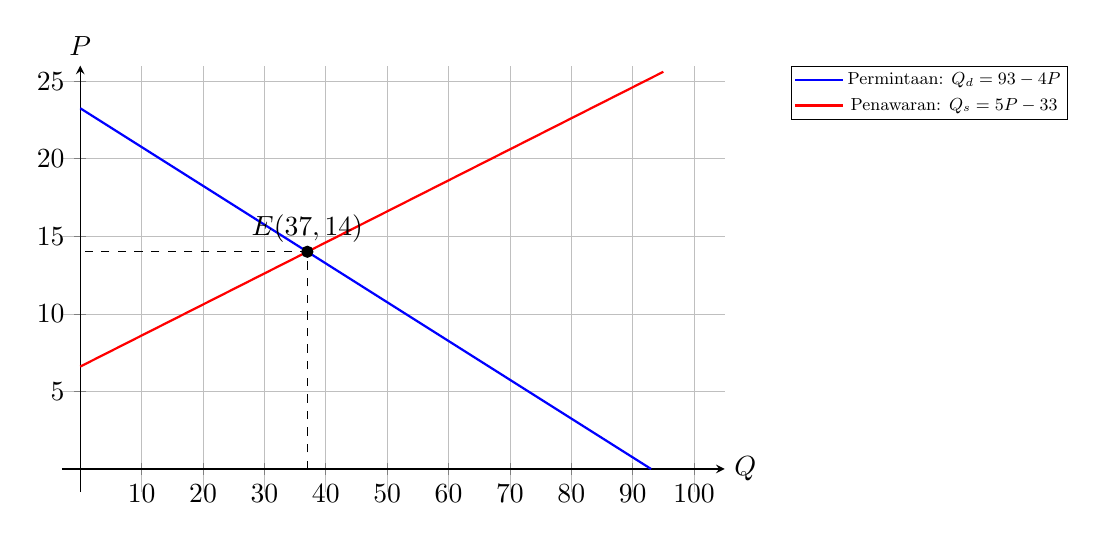
\begin{tikzpicture}
                    \begin{axis}[
        axis lines = middle,
        xlabel = $Q$,
        ylabel = {$P$},
        xtick={0,10,...,100},
        ytick={0,5,...,25},
        xmin=-3, xmax=105,
        ymin=-1.5, ymax=26,
        width=10cm,
        height=7cm,
        grid=both,
        grid style={line width=.1pt, draw=gray!10},
        major grid style={line width=.2pt,draw=gray!50},
        x label style={anchor=west}, % label x ke kanan
        y label style={anchor=south}, % label y ke atas
        samples=200,
        legend style={
                at={(1.1,1)},
                anchor=north west,
                font=\small,         % mengecilkan ukuran font
                row sep=1pt,         % jarak antar baris legend
                inner sep=1pt,       % margin dalam kotak legend
                nodes={scale=0.7}    % skalakan isi legend
            }
    ]
\addplot[domain=0:93, color=blue, thick, samples=2] {(93-x)/4};
\addlegendentry{Permintaan: $Q_d=93-4P$}
\addplot[domain=0:95, color=red, thick, samples=2] {(x+33)/5};
\addlegendentry{Penawaran: $Q_s=5P-33$}
\draw[fill=black] (37,14) circle (2pt) node[above] {$E(37,14)$};
\draw[dashed] (37,0) -- (37,14) -- (0,14);
\end{axis}
                \end{tikzpicture}
            \end{center}
        \end{enumerate}
    }
    \end{jawab}
\end{enumerate}
\newpage

% includepdf hanya dijalankan pada job utama (bukan saat externalize gambar TikZ)
\ifx\pgfactualjobname\tikzexternalrealjob
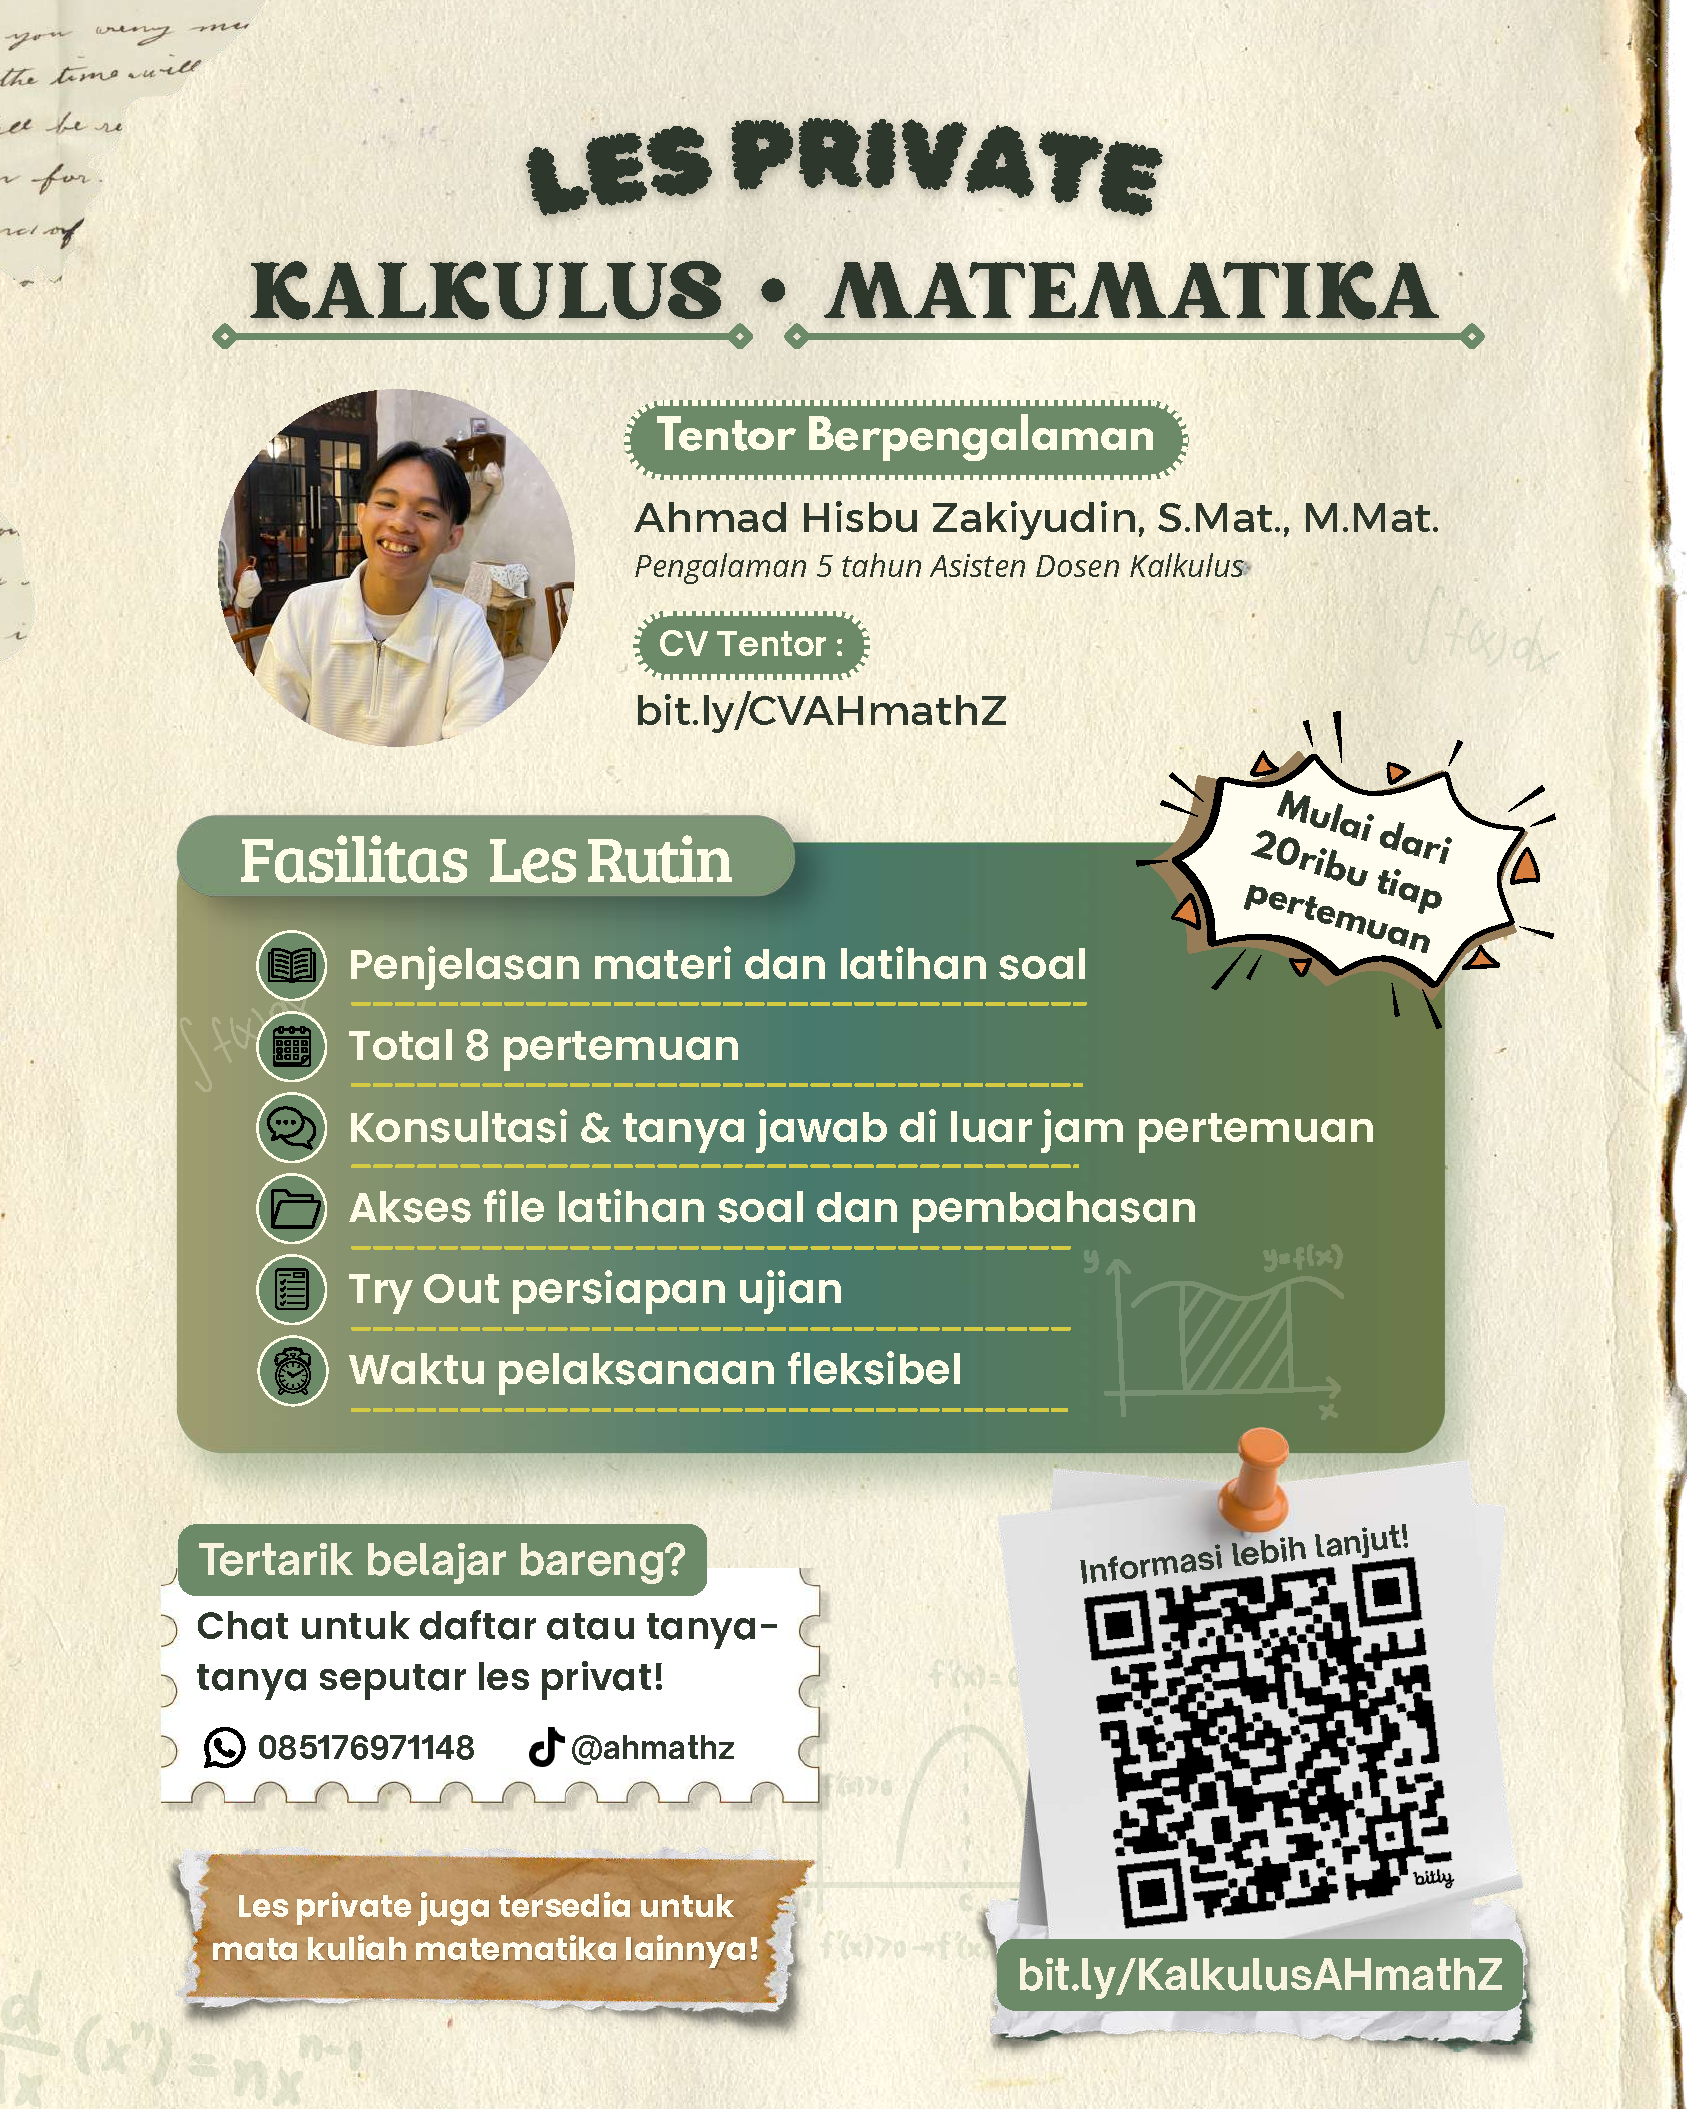
\includepdf[pages=-]{les.pdf}
\fi

\end{document}
